
\pdfoutput=1
\documentclass[11pt]{amsart}
\usepackage[margin=1.0in]{geometry}
\usepackage{amsmath,amssymb,mathtools}
\usepackage{array,booktabs,longtable}
\usepackage{enumitem}
\usepackage{tikz}
\usepackage{adjustbox}
\usepackage{float}
\usepackage{etoolbox}
\usepackage{seqsplit}
\usetikzlibrary{arrows.meta,positioning,shapes.geometric,calc}
\usepackage{pdflscape}
\usepackage{xurl}
\usepackage{microtype}
\usepackage[colorlinks=true,linkcolor=blue,citecolor=blue,urlcolor=blue]{hyperref}
\raggedbottom
\sloppy
\emergencystretch=3em
\setlist{nosep}
\AtBeginEnvironment{longtable}{\footnotesize\sloppy}
\title{Referee Guide to the Navier--Stokes State-Space Stratification Proof}
\author{}
\date{}
\newcommand{\R}{\mathbb{R}}
\newcommand{\calS}{\mathcal{S}}
\newcommand{\calC}{\mathcal{C}}
\newcommand{\capsulefield}[1]{\par\smallskip\noindent\textbf{#1.}\ }
\begin{document}
\maketitle


\section{Executive Summary}

The source files form a single proof architecture for routing and excluding finite-time singularity scenarios for the three-dimensional incompressible Navier--Stokes equations.  The first three files carry the proof-bearing state-space closure, while \path|ns_perelman.tex| provides the localized entropy reformulation of the same closed decision tree.  The organizing principle is to place every possible singular branch in an explicit state-space stratum and then apply the closure theorem whose hypotheses are produced by that stratum.

The proof begins with a finite-energy suitable weak solution

\[
  \partial_t u+(u\cdot\nabla)u+\nabla p=\Delta u,
  \qquad \nabla\cdot u=0,
\]
and assumes that a terminal singular point \(z_*=(x_*,T)\) exists.  Local epsilon-regularity gives the first dichotomy:

\begin{center}
\begin{minipage}{0.92\linewidth}
\scriptsize
\begin{verbatim}
terminal point
  |
  +-- no scale-critical concentration  --> regular by CKN epsilon-regularity
  |
  +-- positive scale-critical concentration
          |
          +-- local pointwise Type I branch
          |
          +-- local Type II branch
\end{verbatim}
\end{minipage}
\end{center}

The proof-bearing papers then close the two positive-concentration branches, and the entropy paper repackages the closed branch ledger as a monotonicity/compactification statement.

\begin{longtable}{@{}>{\raggedright\arraybackslash}p{0.25\linewidth}>{\raggedright\arraybackslash}p{0.35\linewidth}>{\raggedright\arraybackslash}p{0.32\linewidth}@{}}
\toprule
\textbf{Paper} & \textbf{Role in the architecture} & \textbf{Main output} \\
\midrule
\endhead
\path|proof_setup.tex| & Establishes local concentration, the Type I/Type II dichotomy, Type I Seregin extraction, and the first non-residual Type I class closures. & A local pointwise Type I singularity produces a nonzero normalized bounded centered ancient Seregin profile. That profile is either in a closed non-residual Liouville class or in the residual class. \\
\path|paperIV_residual_branch.tex| & Refines and closes the Type I residual class left by the setup paper. & The retained normalized residual class is empty after an ordered residual decomposition into axisymmetric, rotational, stationary-hull, affine/parasitic, critical-tail, and generic terminal strata. \\
\path|type_II_regularity.tex| & Excludes the local Type II branch by closing every state-space exit. & Every positive local Type II concentration sequence enters one of the repaired-gauge, multibubble, rough-core, scale-collapse, retained compact-cost, carrier-routing, or terminal-profile alternatives; scale-rigidity, windowwise routing, cost-divergence, analytic-data exhaustion, retained compact-test closure, and critical-profile completeness are all discharged inside the paper. \\
\path|ns_perelman.tex| & Recasts the closed companion state-space program in localized entropy language. & The localized entropy has one-sided limits up to controlled error; entropy-critical limits reduce to the already closed terminal model classes, and the companion exclusions eliminate those classes without adding a new PDE closure assumption. \\
\bottomrule
\end{longtable}

The resulting architecture is:

\begin{center}
\begin{minipage}{0.92\linewidth}
\scriptsize
\begin{verbatim}
finite-energy suitable weak solution
  |
  +-- suppose a singular point exists
          |
          +-- local CKN concentration gives positive critical mass
                  |
                  +-- Type I branch
                  |     |
                  |     +-- Seregin ancient limit
                  |     +-- non-residual Liouville classes closed in proof_setup.tex
                  |     +-- residual classes closed in paperIV_residual_branch.tex
                  |     +-- contradiction
                  |
                  +-- Type II branch
                        |
                        +-- repaired-gauge/local-profile state-space partition
                        +-- all Type II state-space exits closed in type_II_regularity.tex
                        +-- contradiction
\end{verbatim}
\end{minipage}
\end{center}

For verification, each branch is listed with the theorem package that supplies its hypotheses and the theorem package that closes it.  The Type I residual closure is discharged by \path|paperIV_residual_branch.tex|, including the setup residual hypothesis.  In \path|type_II_regularity.tex|, the principal interface conditions are implemented as theorem or corollary packages: \path|paper3:prop:local-scale-rigidity-exclusion|, \path|paper6:thm:bounded-selected-window-physical-routing|, \path|paper6:thm:ordered-local-state-space-exhaustion|, \path|paper6:cor:remaining-named-exits-closed|, \path|paper7:cor:windowwise-transition-routing-holds|, \path|paper7:cor:windowwise-positive-scale-routing-holds|, \path|paper6a:thm:local-residual-exhaustion|, \path|paper6a:thm:cost-divergence-exclusion-discharged|, \path|paper6a:thm:critical-ns-profile-decomposition-discharged|, and the \path|paper9| critical-tail closure package.  The Type II ledger is closed: entry into the local alternative class, repaired-gauge representation, compactness and local energy propagation, bounded-window reselection, retained compact-test closure, cost/carrier routing, critical-tail routing, terminal profile exhaustion, and all remaining named exits are supplied by named theorem packages in \path|type_II_regularity.tex|.  The entropy paper imports this companion package through \path|thm:companion-package| and closes its entropy-critical terminal classes by \path|thm:five-classes-ordered| and \path|thm:eliminate-terminal-classes|.

\section{Scope and Verification Protocol}

The document has four functions.
\begin{enumerate}
\item It identifies the proof-bearing files and the entropy reformulation.
\item It records every state-space exit and its closure theorem package.
\item It records every interface where hypotheses pass from one paper to another.
\item It provides a source-generated theorem label register for checking that the architecture paper refers to the TeX sources.
\end{enumerate}

Verification proceeds against the source files in the following order: first the entry and Type I extraction statements in \path|proof_setup.tex|; then the residual closure in \path|paperIV_residual_branch.tex|; then the Type II state-space, cost/carrier, terminal, and remaining-exit closures in \path|type_II_regularity.tex|; and finally the entropy reformulation in \path|ns_perelman.tex|.  A row is complete only when its entry hypotheses, retained obstruction, rerouting rule, and terminal contradiction are all supplied by cited statements.

\section{Auditable Capsule View}
\label{sec:auditable-capsule-view}

This section records the Navier--Stokes-specific proof-capsule material that is
used as the case study for the general auditable-proof protocol.  The point is
architectural: global regularity is organized by exhausting local singularity
branches rather than by propagating one whole-space critical norm through the
proof.

\subsection{One-Page Routing Graph}

\begin{center}
\begin{minipage}{0.92\linewidth}
\scriptsize
\begin{verbatim}
terminal singular branch
  -> concentration gate
      -> no concentration: regularity
      -> positive concentration
          -> Type I envelope
              -> Seregin ancient state
              -> direct Liouville classes or residual class
          -> Type II branch
              -> repaired gauge / local state-space alternatives
              -> compact core, rough core, multibubble, cascade,
                 scale collapse, carrier, terminal profile, exterior exits
\end{verbatim}
\end{minipage}
\end{center}

This flow diagram is the abstract syntax tree of the proof: once a branch enters
the tree, every future estimate is attached to a named local state and every
terminal trap is tied to a retained obstruction.

\subsection{Representative Capsule Ledger}

\begin{center}
\scriptsize
\begin{longtable}{@{}p{0.14\linewidth}p{0.17\linewidth}p{0.17\linewidth}p{0.14\linewidth}p{0.20\linewidth}@{}}
\toprule
Capsule & Input & Output & Retained obstruction & Failure route/status \\
\midrule
Concentration gate & suitable weak solution with candidate singular point & positive local critical concentration or regularity & CKN or velocity mass & epsilon-regularity closure; imported or closed \\
Type I extraction & local Type I envelope plus retained mass & bounded ancient profile & compact local \(L^3\) mass & residual ancient state; imported or closed \\
Type II repaired gauge & retained moving core & represented local equation on compact window & core concentration & gauge-degenerate, rough-core, multibubble exits; row status recorded \\
Terminal profile route & compact terminal sequence with retained mass & profile extraction or perturbative remainder & terminal critical mass & hidden-mass or profile-exhaustion exit; row status recorded \\
\bottomrule
\end{longtable}
\end{center}

\subsection{Worked Capsule: Concentration Entry}

\capsulefield{Capsule name}
Concentration entry.

\capsulefield{Input contract}
\begin{itemize}
  \item A finite-time candidate singular point for a suitable weak Navier--Stokes solution in the standard local energy framework of Leray and Caffarelli--Kohn--Nirenberg.
\end{itemize}

\capsulefield{Output contract}
\begin{itemize}
  \item Either the branch is regular by epsilon-regularity, or a scale-invariant local concentration lower bound survives along a sequence of shrinking parabolic cylinders.
\end{itemize}

\capsulefield{Retained obstruction}
\begin{itemize}
  \item Positive CKN or velocity concentration at the candidate singular point.
\end{itemize}

\capsulefield{Failure routes}
\begin{itemize}
  \item Vanishing concentration routes to regularity.
  \item Pressure-normalization ambiguity routes to the pressure/gauge audit row.
  \item Failure of suitable-weak-solution hypotheses routes to an imported-existence/input-status node.
\end{itemize}

\capsulefield{Audit checks}
\begin{itemize}
  \item Scaling invariance of the concentration quantity.
  \item Pressure gauge normalization.
  \item Exact epsilon-regularity threshold.
  \item Preservation of the lower bound under subsequence extraction.
  \item Dependency on only the declared local cylinder.
\end{itemize}

\subsection{Verification Ledgers}

\begin{center}
\begin{tabular}{p{0.23\linewidth}p{0.31\linewidth}p{0.31\linewidth}}
\toprule
Interface & Source output & Target input \\
\midrule
Concentration gate & positive critical mass & Type I/Type II routing \\
Type I extraction & bounded ancient profile with retained mass & direct classes or residual class \\
Residual routing & realized descendant or terminal state & matching residual closure capsule \\
Type II entry & retained moving core & repaired-gauge representation \\
Gauge representation & local equation with modulation and pressure atlas & compactness, Caccioppoli, cost, and carrier capsules \\
Terminal profile route & retained terminal mass & profile extraction or hidden-mass exit \\
\bottomrule
\end{tabular}
\end{center}

\begin{center}
\begin{longtable}{p{0.25\linewidth}p{0.35\linewidth}p{0.30\linewidth}}
\toprule
Obstruction & Produced by & Contradicted by \\
\midrule
positive CKN mass & concentration gate & epsilon-regularity or vanishing pressure/velocity \\
compact local \(L^3\) mass & Seregin extraction & Liouville zero conclusion \\
residual ancestry & descendant realization & closure of non-realized auxiliary objects is disallowed \\
retained Type II core mass & selected core construction & compact zero limit or finite-cost collapse \\
carrier cost & local cost validation & corrected monotonicity plus carrier routing \\
terminal critical mass & terminal profile extraction & profile exhaustion and perturbative remainder \\
\bottomrule
\end{longtable}
\end{center}

\subsection{Capsule Examples}

\capsulefield{Capsule name}
Selected-window compactness extraction.

\capsulefield{Implementation labels}
\begin{itemize}
  \item L1. \path|paper1:prop:compactness|.
  \item L2. \path|paper1:lem:D-localization| for the smaller-cylinder pressure bound used inside the compactness proof.
\end{itemize}

\capsulefield{Source}
Proposition ``Compactness on selected windows'' in the companion Type II
manuscript.

\capsulefield{Input contract}
\begin{itemize}
  \item H1. A represented suitable sequence on \(Q_{R_*}\) solving the local renormalized equation.
  \item H2. Uniform compact-cylinder bounds \(A_{V_n}(R_*)+E_{V_n}(R_*)+C_{V_n}(R_*)+D_{P_n}(R_*)\le M\).
  \item H3. Uniformly bounded modulation coefficients \(a_n,b_n\) on the selected time interval.
\end{itemize}

\capsulefield{Output contract}
\begin{itemize}
  \item O1. For every \(r<R_*\), a subsequence converges weak-* in \(L^\infty_tL^2_x\), weakly in \(L^2_tH^1_x\), and strongly in \(L^3(Q_r)\).
  \item O2. Mean-normalized pressure converges weakly in \(L^{3/2}(Q_r)\), and the limit still satisfies the represented equation distributionally on smaller cylinders.
\end{itemize}

\capsulefield{Retained obstruction}
\begin{itemize}
  \item I. The capsule transports the branch into a compactness topology strong enough for later retention and contradiction capsules.
\end{itemize}

\capsulefield{Failure routes}
\begin{itemize}
  \item F1. If the local pressure oscillation bound is unavailable, route to a pressure-row or pressure-compactness failure state.
  \item F2. If bounded modulation or time-derivative control fails, route to modulation-failure or compactness-failure states rather than invoking compactness implicitly.
\end{itemize}

\capsulefield{Audit checklist}
\begin{itemize}
  \item A1. Check the pressure is normalized by spatial means on each compact ball.
  \item A2. Check the \(L^2\) to \(L^3\) interpolation and the use of the \(L^{10/3}\) bound.
  \item A3. Check weak-* convergence for \(a_n,b_n\) is sufficient for passage to the limit in the lower-order terms.
  \item A4. Check the argument never upgrades local compact-cylinder data into a hidden whole-space compactness theorem.
\end{itemize}

\capsulefield{Closure status}
Open as a transport capsule; it is an upstream interface rather than a terminal
contradiction.

\capsulefield{Capsule name}
Local single-core Type II exclusion.

\capsulefield{Implementation labels}
\begin{itemize}
  \item L1. \path|paper1:thm:single-core-criterion|.
  \item L2. \path|paper1:lem:zero-dissipation| for the constant-limit reduction.
  \item L3. \path|paper1:lem:zero-contradiction| for the zero-limit contradiction.
  \item L4. \path|paper1:lem:nonzero-contradiction| for the bounded-window exit.
\end{itemize}

\capsulefield{Source}
Theorem ``Local single-core Type II criterion'' in the companion Type II
manuscript.

\capsulefield{Input contract}
\begin{itemize}
  \item H1. A compact single-core vanishing-dissipation branch in the precise sense of the Type II manuscript.
  \item H2. Upstream access to the named inputs ``passage to selected-window branches,'' ``local representation input,'' and ``local pressure reconstruction.''
  \item H3. Persistence of a selected retained core with positive concentration on \(Q_{r_*}\).
\end{itemize}

\capsulefield{Output contract}
\begin{itemize}
  \item O1. The branch cannot remain a local Type II sequence.
  \item O2. Any nonzero bounded selected-window limit is rerouted to the bounded-window row instead of remaining inside the strict selected-window branch.
\end{itemize}

\capsulefield{Retained obstruction}
\begin{itemize}
  \item I. Positive retained velocity concentration on the selected core, encoded by a fixed lower bound \(C_{V_n}(r_*)\ge \eta_0\) along the selected-window subsequence.
\end{itemize}

\capsulefield{Failure routes}
\begin{itemize}
  \item F1. If the limit is spatially constant and nonzero, exit the strict selected-window Type II branch through the bounded-window routing row.
  \item F2. Multibubble, cascade, gauge-degenerate, and compactness-failure alternatives are separate named rows outside the single-core capsule.
\end{itemize}

\capsulefield{Audit checklist}
\begin{itemize}
  \item A1. Check the vanishing localized dissipation really implies a spatially constant limit on the selected compact cylinder.
  \item A2. Check the strong \(L^3\) convergence on the core cylinder is exactly what forces the zero-limit contradiction.
  \item A3. Check the retained obstruction is contradicted only in the zero-constant case and rerouted rather than contradicted in the nonzero-constant case.
  \item A4. Check no hidden stationary, ancient, or self-similar Liouville theorem is invoked.
\end{itemize}

\capsulefield{Closure status}
Closed terminal exclusion capsule inside the local single-core row, with named
exits for behavior that leaves that row.

\subsection{Routing Skeleton}

\begin{center}
\begin{minipage}{0.92\linewidth}
\scriptsize
\begin{verbatim}
finite-energy suitable weak solution
  -> suppose terminal singular point exists
      -> concentration gate
          -> no concentration: epsilon-regularity closure
          -> positive concentration
              -> Type I envelope?
                  yes: Seregin ancient-profile state space
                  no: Type II retained local-window state space

Type I branch
  -> Seregin extraction
      -> small class: perturbative Liouville
      -> stationary L3 class: stationary rigidity
      -> uniformly tight class: endpoint ancient Liouville
      -> structure/decay class: specialized Liouville theorem
      -> residual class: residual terminal-dynamics graph

Type II branch
  -> select retained moving core
      -> repaired gauge representation
      -> compact single core
      -> rough core / H1 loss
      -> multibubble / cascade / gauge degeneracy
      -> scale collapse / finite cost / carrier routing
      -> terminal critical profile / exterior states
\end{verbatim}
\end{minipage}
\end{center}

\section{Provenance and Audit Standard}

This guide is an audit layer over the source files; it is not an independent proof source.  A branch is recorded as closed only when the source contains a named statement that supplies the entry hypotheses, preserves the retained obstruction through the required compactness or gauge operation, and produces the terminal contradiction or a named downstream route.

The trust standard used throughout the guide is:

\begin{longtable}{@{}>{\raggedright\arraybackslash}p{0.26\linewidth}>{\raggedright\arraybackslash}p{0.36\linewidth}>{\raggedright\arraybackslash}p{0.30\linewidth}@{}}
\toprule
\textbf{Audit item} & \textbf{Required check} & \textbf{Where recorded} \\
\midrule
\endhead
Source ownership & Each closure is attributed to \path|proof_setup.tex|, \path|paperIV_residual_branch.tex|, \path|type_II_regularity.tex|, \path|ns_perelman.tex|, or an explicitly cited external theorem inside those files. & Closure status tables, edge audit tables, and capsule sources. \\
Entry hypotheses & The upstream routing theorem produces the hypotheses used by the downstream closure theorem. & Diagram edge audit and per-node input contracts. \\
Retained obstruction & The positive concentration, retained compact \(L^3\) mass, residual ancestry, Type II core mass, or entropy-critical obstruction survives every limit used in the row. & Retained-obstruction tables and capsule audit checklist. \\
Failure containment & If a hypothesis of a closure row fails, the failure is routed to a named state-space row rather than left as an unclassified remainder. & Complete exit ledger and capsule failure routes. \\
Label traceability & The theorem register lists the theorem-environment labels from the four source files and separately records the theorem-style proposition label \path|paper2:thm:quant-jac| used by the Type II representation package. & Complete theorem label register. \\
\bottomrule
\end{longtable}

Thus a referee can audit any terminal row by following this sequence: locate the row in the exit ledger, check its incoming edge in the diagram audit, verify the corresponding capsule input and output contracts, and then inspect the named source theorem.  The guide requires revision whenever a source theorem is renamed, removed, weakened, or replaced by a different closure mechanism.

\section{Closure Status}

The proof-bearing state space is closed as follows.

\begin{longtable}{@{}>{\raggedright\arraybackslash}p{0.25\linewidth}>{\raggedright\arraybackslash}p{0.35\linewidth}>{\raggedright\arraybackslash}p{0.32\linewidth}@{}}
\toprule
\textbf{Branch or interface} & \textbf{Status} & \textbf{Closing theorem package} \\
\midrule
\endhead
Vanishing local concentration & Closed. & \path|p0:thm:ckn|, \path|p0:thm:velocity-ckn|, \path|p0:thm:no-concentration|. \\
Local pointwise Type I, non-residual classes & Closed. & \path|p1:thm:classical-classes|, \path|p2:thm:NRS|, \path|p1:thm:tight-liouville|, \path|p1:thm:known-structure-decay-liouville|, and the Part III/IV Liouville packages in \path|proof_setup.tex|. \\
Type I residual class & Closed. & \path|thm:paperIV-residual-closure|, with \path|cor:setup-residual-hypothesis-proof| feeding back into the setup paper. \\
Type II entry and analytic-data exhaustion & Closed. & \path|paper6:thm:paper0|, \path|thm:c1-typeII-branch-exhaustion|, \path|paper6:thm:physical-typeII-covered-entry|, \path|paper6a:thm:typeII-analytic-data-exhaustive|. \\
Repaired-gauge representation and pressure/local-energy compatibility & Closed. & \path|paper6:thm:representation|, \path|paper2:thm:quant-jac|, \path|thm:c2-representation-implication|, \path|thm:c2r-minimal-representation|, \path|paper6a:thm:ac-repaired-gauge-consequences|. \\
Compact single core, rough core, multibubble, and cascade exits & Closed. & \path|paper6:thm:single-core|, \path|paper6:thm:rough-core|, \path|paper6:thm:multibubble|, \path|paper7:thm:windowed-h1-failure-exclusion|, and the same-point cascade theorems. \\
Scale collapse and scale-rigidity exits & Closed. & \path|paper6:thm:scale-cost|, \path|paper6:thm:scale-stratification|, \path|paper6:prop:state-elimination|, \path|paper3:prop:scale-rigidity-discharged|. \\
Retained compact cost and carrier exits & Closed. & \path|paper7:thm:classwise-retained-compact-coverage|, \path|paper7:thm:windowwise-routing-gives-stratified-routing|, \path|paper7:def:stratified-moving-carrier-routing|, \path|paper6a:thm:cost-divergence-exclusion-discharged|. \\
Bounded-window, noncanonical-cost, and active-core-loss adjacent exits & Closed. & \path|paper6:thm:bounded-selected-window-physical-routing|, \path|paper6:thm:autonomous-modulation-failure-closed|, \path|paper6:thm:noncanonical-cost-routing-closed|, \path|paper6:thm:active-core-loss-closed|, \path|paper6:cor:remaining-named-exits-closed|. \\
Terminal hidden critical profile, diffuse critical tail, and residual mass exits & Closed. & \path|paper6a:thm:local-residual-exhaustion|, \path|paper6a:thm:critical-ns-profile-decomposition-discharged|, \path|paper6a:thm:retained-compact-tests-closed|, \path|paper6a:thm:terminal-critical-local-compactness|, \path|paper9:thm:logarithmic-tail-support-transfer|, \path|paper9:thm:minimal-mesoscopic-extraction|, \path|paper9:thm:young-variance-strong-compactness|, \path|paper9:thm:coherent-critical-tail-closure|, \path|paper6a:thm:expanded-terminal-typeII|. \\
Final Type II assembly & Closed. & \path|paper6:thm:ordered-local-state-space-exhaustion|, \path|paper6:thm:state-decomposition|, \path|paper6:prop:state-elimination|, \path|paper6:thm:unconditional-no-typeII|, \path|paper6:thm:unconditional-no-typeII-discharged|, \path|paper6:thm:local-typeII-exclusion|. \\
Entropy reformulation & Closed as a reformulation of the companion closure. & \path|thm:intro-main|, \path|thm:companion-package|, \path|thm:local-monotonicity|, \path|thm:zero-gradient-recovery|, \path|thm:five-classes-ordered|, \path|thm:eliminate-terminal-classes|, \path|cor:entropy-reformulation|. \\
\bottomrule
\end{longtable}

The final proof is organized around a finite routing graph whose terminal nodes are contradictions: local regularity contradicts the choice of singular point, a Liouville theorem contradicts retained Type I mass, the residual state space is empty, or a Type II exit contradicts retained core mass, finite cost, scale-rigidity closure, or terminal profile exhaustion.

\section{Complete Exit and Rerouting Ledger}
\label{sec:complete-exit-ledger}

The tables in this section form the verification ledger for the proof.  Each row records an exit, the routing test that sends a branch there, whether the exit terminates directly or reroutes to another exit, and the closure mechanism.  The entries are more explicit than the diagrams so that the proof can be checked one branch at a time.

\subsection{Global and Setup Exits}

\begin{longtable}{@{}>{\raggedright\arraybackslash}p{0.19\linewidth}>{\raggedright\arraybackslash}p{0.25\linewidth}>{\raggedright\arraybackslash}p{0.28\linewidth}>{\raggedright\arraybackslash}p{0.20\linewidth}@{}}
\toprule
\textbf{Exit} & \textbf{Entry test} & \textbf{Routing or rerouting mechanism} & \textbf{Closure} \\
\midrule
\endhead
Vanishing CKN concentration & The scale-invariant \(C+D\) quantity becomes small at the candidate terminal point. & No further blow-up analysis is permitted; the branch exits to local regularity. & \path|p0:thm:ckn| and \path|p0:thm:no-concentration| give local boundedness, contradicting singularity. \\
Vanishing velocity concentration & The velocity-only critical quantity \(C\) vanishes along the candidate singular scales. & Routed to velocity epsilon-regularity rather than Seregin or Type II extraction. & \path|p0:thm:velocity-ckn| closes the branch. \\
Positive concentration with local pointwise Type I envelope & Positive local critical mass persists and the Type I scale-invariant \(L^\infty\) envelope is finite. & Routed into the Type I bridge sequence and Seregin extraction. & \path|p0:thm:local-weak-serrin-typeI|, \path|p1:thm:extraction|, and the Type I class ledger below. \\
Positive concentration with no local pointwise Type I envelope & Positive local critical mass persists but every local Type I envelope fails. & Routed into the Type II local state-space assembly. & \path|p0:thm:typeI-typeII-dichotomy|, \path|paper6:thm:paper0|, \path|paper6:thm:physical-typeII-covered-entry|, and the Type II ledger below. \\
Terminal velocity no-escape failure & A Type I bridge sequence would lose velocity mass into the terminal slice. & Routed back to the local weak-Serrin/no-escape estimates before extraction. & \path|p0:thm:auto-velocity-no-escape| and \path|p0:thm:local-weak-serrin-typeI| restore admissibility or close the branch. \\
Setup residual hypothesis & The setup paper reaches the residual Type I class after direct Liouville classes are removed. & Routed to \path|paperIV_residual_branch.tex| as the imported residual object. & \path|thm:paperIV-residual-closure| and \path|cor:setup-residual-hypothesis-proof| close the setup residual hypothesis. \\
\bottomrule
\end{longtable}

\subsection{Direct Type I Exits}

\begin{longtable}{@{}>{\raggedright\arraybackslash}p{0.19\linewidth}>{\raggedright\arraybackslash}p{0.25\linewidth}>{\raggedright\arraybackslash}p{0.28\linewidth}>{\raggedright\arraybackslash}p{0.20\linewidth}@{}}
\toprule
\textbf{Exit} & \textbf{Entry test} & \textbf{Routing or rerouting mechanism} & \textbf{Closure} \\
\midrule
\endhead
Small-amplitude Seregin profile & The normalized centered ancient profile is small in the relevant scale-invariant topology. & No residual routing; perturbative rigidity applies immediately. & \path|p1:thm:classical-classes| forces zero, contradicting retained compact \(L^3\) mass. \\
Stationary \(L^3\) Seregin profile & A time-translate or representative is stationary with critical \(L^3\) control. & Routed to stationary self-similar rigidity. & \path|p1:thm:classical-classes| and \path|p2:thm:NRS| force zero. \\
Uniformly \(L^3\)-tight Seregin profile & The ancient trajectory keeps its \(L^3\) mass uniformly tight in space. & Routed through physical pullback and endpoint sequence-\(L^3\) construction. & \path|p2:thm:tight-liouville|, \path|p2:thm:AB-endpoint|, and \path|p1:thm:tight-liouville| force zero. \\
Structured or decay-covered Seregin profile & Axisymmetry, no-swirl, pointwise scale control, weighted-vorticity smallness, or another listed structure is present. & Routed to the matching structure-specific Liouville theorem. & \path|p3:thm:axisymmetric-liouville|, \path|p3:thm:typeI-zero-hypotheses|, and \path|p1:thm:known-structure-decay-liouville| force zero. \\
Direct Type I class exhaustion failure & A profile avoids all direct classes. & The complement is identified with the residual class. & Routed to the residual ledger by \path|p1:thm:remaining-criterion|. \\
\bottomrule
\end{longtable}

\subsection{Type I Residual Exits}

\begin{longtable}{@{}>{\raggedright\arraybackslash}p{0.19\linewidth}>{\raggedright\arraybackslash}p{0.25\linewidth}>{\raggedright\arraybackslash}p{0.28\linewidth}>{\raggedright\arraybackslash}p{0.20\linewidth}@{}}
\toprule
\textbf{Exit} & \textbf{Entry test} & \textbf{Routing or rerouting mechanism} & \textbf{Closure} \\
\midrule
\endhead
Imported residual object mismatch & The residual paper must use the same Seregin object produced by setup. & The imported setup package fixes the object, retained mass, pressure gauge, and ancestry. & \path|thm:imported-setup-results| and \path|hyp:base-seregin-hypotheses| align the interface. \\
Non-realized descendant & A recentered limit, hull element, tail state, or terminal profile must descend from the original branch. & Routed through ancestor-realization and heredity before any closure theorem is applied. & \path|thm:ancestor-realization-inheritance| and \path|thm:descendant-heredity| make descendant closures logically effective. \\
Axisymmetric bounded-circulation residual & The residual profile is axisymmetric with bounded centered circulation after lower direct classes are removed. & Routed through centered circulation and axis-absorption; if it falls into no-swirl or lower structured behavior, it is sent back to direct Type I closure. & \path|thm:R1-exclusion| closes the exit. \\
Rotational relative equilibrium & The residual profile is stationary modulo rotation and carries local Coriolis transport structure. & Routed through local Coriolis flux and terminal concentration; lower compact profiles are sent to already closed strata. & \path|prop:R2-reduction-to-terminal|, \path|thm:terminal-stratification|, and \path|cor:R2-closure| close the exit. \\
Degenerate stationary hull & A time-translation hull contains a degenerate stationary-family carrier with retained concentration. & Routed through stationary-family realization, terminal stratification, and no-active-stationary-carrier closure. & \path|thm:R3-no-attainable-degenerate-family|, \path|thm:R3S-terminal-theorem|, and \path|thm:R3S-no-active-stationary-carrier|. \\
Affine or parasitic quotient & The apparent residual behavior is an affine/parasitic normalization mode rather than genuine nonlinear retained activity. & Routed through affine normalization; oscillatory representatives are removed and non-oscillatory representatives drop to lower strata. & \path|thm:affine-normalization-dichotomy| and \path|thm:oscillatory-entry-normalization|. \\
Closed non-affine activity failure & The non-affine active set must be closed under the local observer calculus. & Routed through covariant observers and hull compactness before terminal extraction. & \path|thm:covariant-observer-calculus|, \path|thm:closed-nonaffine-activity|, and \path|thm:escaping-covariant-hull-compactness|. \\
Recurrent tail-core residual & Tail activity recurs without entering a compact terminal profile. & Routed to recurrent tail-core rigidity or to terminal concentration extraction. & \path|thm:recurrent-tail-core-rigidity| and \path|thm:terminal-exhaustion-main|. \\
Log-diffuse critical tail & Critical activity escapes through logarithmic annuli. & Routed to hidden-scale compactification and then to critical-tail compactification. & \path|thm:log-diffuse-from-hidden-scale| and \path|thm:critical-tail-compactification-extraction|. \\
Young critical-tail defect & Tail mass survives only as a variance or Young-measure defect. & Routed to first bad mesoscopic scale; realized hidden variance is excluded before compactification. & \path|thm:first-bad-mesoscopic-reduction| and \path|thm:no-hidden-scale-variance-realized-defects|. \\
Coherent homogeneous critical tail & Tail compactification produces a coherent homogeneous critical state. & Routed through bounded-origin realization; realized homogeneous tails become incompatible with bounded residual origin behavior. & \path|thm:coherent-critical-tail-classification|, \path|thm:bounded-origin-realization-coherent-tails|, and \path|thm:realized-critical-tail-rigidity|. \\
Coherent log-periodic critical tail & Tail compactification produces a coherent log-periodic state. & Routed to the same coherent-tail classification and realization test. & \path|thm:coherent-critical-tail-classification| and \path|thm:realized-critical-tail-rigidity|. \\
Coherent aperiodic critical tail & Tail compactification produces a compact log-translation hull with no period. & Routed to the aperiodic coherent-tail rigidity branch. & \path|thm:coherent-critical-tail-classification| and \path|thm:realized-critical-tail-rigidity|. \\
Terminal nonactive or nonconcentrating state & Terminal extraction produces no active compact concentration. & Routed to terminal nonactive discharge; retained mass cannot disappear. & \path|thm:terminal-inactive-exclusion|. \\
Diffuse terminal defect & Terminal mass is diffuse rather than carried by a compact active profile. & Routed through diffuse compactness, recurrent diffuse measures, and the diffuse trichotomy; active outputs re-enter active terminal routing, affine outputs re-enter affine closure, tail outputs re-enter critical-tail closure. & \path|thm:diffuse-defect-compactness|, \path|thm:recurrent-diffuse-defect-measure|, and \path|thm:diffuse-defect-trichotomy|. \\
Mixed compact-diffuse terminal mass & Compact active concentration and diffuse defect coexist without a clean decomposition. & Routed to the mixed compact-diffuse exclusion. & \path|thm:no-mixed-compact-diffuse|. \\
Finite separated active profile family & Terminal mass splits into finitely many separated compact active profiles. & Routed through separated-profile analysis and indecomposability. & \path|thm:no-finite-separated-profile-family|. \\
Infinite active descendant chain or recurrence loop & Retained activity keeps regenerating through descendants without terminal closure. & Routed to active path-space recurrence and compact active descendant extraction. & \path|thm:active-path-space-recurrence| and \path|thm:compact-active-descendant|. \\
Generic terminal residual & No lower residual, tail, affine, diffuse, separated, or recurrent exit remains. & Routed through parasitic-free mildness, sequence-\(L^3\) completeness, and endpoint Liouville. & \path|thm:mildness-inheritance-main|, \path|thm:AB-main|, \path|thm:R4-final-closure|, and \path|thm:paperIV-residual-closure|. \\
\bottomrule
\end{longtable}

\subsection{Type II Exits}

\begin{longtable}{@{}>{\raggedright\arraybackslash}p{0.19\linewidth}>{\raggedright\arraybackslash}p{0.25\linewidth}>{\raggedright\arraybackslash}p{0.28\linewidth}>{\raggedright\arraybackslash}p{0.20\linewidth}@{}}
\toprule
\textbf{Exit} & \textbf{Entry test} & \textbf{Routing or rerouting mechanism} & \textbf{Closure} \\
\midrule
\endhead
Type II analytic-data failure & A positive Type II branch lacks the analytic data needed for the local assembly. & Routed through the C1/C3/C4/C5 PDE-form classification until either analytic data are produced or a cost/annulus alternative fires. & \path|thm:c1-typeII-branch-exhaustion|, \path|cor:c1-ordered-exhaustion|, \path|paper6a:thm:typeII-analytic-data-exhaustive|. \\
Repaired-gauge representation failure & A retained core cannot be put into a stable scale-center chart. & Routed to minimal representation, multibubble, cascade, or scale-rigid alternatives. & \path|paper6:thm:representation|, \path|paper2:thm:quant-jac|, \path|thm:c2-representation-implication|, \path|thm:c2r-minimal-representation|. \\
Pressure or local-energy incompatibility in repaired variables & The transformed branch must remain suitable and pressure-stable. & Routed through pressure decomposition, AC repaired-gauge consequences, and local Caccioppoli estimates. & \path|paper2:thm:pressure-decomp|, \path|paper2:thm:A|, \path|paper2:thm:B|, \path|paper2:thm:C|, \path|paper6a:thm:ac-repaired-gauge-consequences|. \\
Compact single-core branch & One retained core persists with compact-window control and vanishing localized dissipation. & If the limit is zero, retained mass is lost; if nonzero bounded, the branch exits Type II into Type I-type bounded behavior. & \path|paper1:thm:single-core-criterion| and \path|paper6:thm:single-core|. \\
Bounded selected-window row & A selected-window subsequence has a bounded local profile before the physical routing layer has assigned it to a retained or adjacent state. & Routed through local regularity, pressure/VMO checks, diffuse reselection-tree well-foundedness, or a named adjacent row. & \path|paper3:lem:scale-rigid-bounded-limit-exit|, \path|paper6:thm:bounded-selected-window-physical-routing|, and the \path|paper10| reselection-tree package. \\
Windowed \(H^1\) or rough-core failure & A selected core has critical mass but lacks inner gradient control. & Routed through Caccioppoli; failure of outer compact-cylinder control re-enters compactness failure, multibubble, or cascade exits. & \path|paper4:thm:caccioppoli|, \path|paper7:thm:windowed-h1-failure-exclusion|, \path|paper6:thm:rough-core|. \\
Same-point comparable-scale multibubble & Several active profiles occur near the same point and comparable scales. & Routed through active-frame reduction, thresholded mass counting, and terminal decoupling. & \path|paper3:thm:multi|, \path|paper8:thm:multibubble-frame-reduction|, \path|paper6:thm:multibubble|. \\
Same-point strict scale cascade & Active profiles occur at the same point on separated scales. & Routed through same-point reduction, scale separation, and terminal decoupling; irregular cascades reroute to rough-core or scale-rigid exits. & \path|paper3:thm:same-point-reduction|, \path|paper8:thm:same-point-scale-separation|, \path|paper8:thm:terminal-decoupling-implies-local-decoupling|. \\
Separated-point multibubble & Active profiles occur at separated centers. & Routed through local pressure and mass decoupling; each component returns to compact-core, terminal-profile, or small-data closure. & \path|paper3:thm:separated-point-reduction|, \path|paper8:thm:terminal-decoupling-implies-local-decoupling|. \\
Gauge-degenerate branch & The selected chart is nonunique or unstable because several cores or scales compete. & Routed to multibubble, same-point cascade, separated-profile, or scale-rigid exits. & Closed by \path|paper6:thm:state-decomposition| after the target exit closes. \\
Finite scale-collapse cost & The selected scale collapses but the signed or absolute scale cost is finite. & No reroute: retained core mass forces infinite cost. & \path|paper5:thm:cost-exclusion|, \path|paper6a:thm:scale-collapse-drift-cost|, \path|paper6:thm:scale-cost|. \\
Collapse core-floor failure & A collapsing branch must retain a nonzero localized core. & Routed to vanishing critical \(L^3\) or terminal compactness closure. & \path|paper5:thm:collapse-core-floor|, \path|paper6a:thm:collapse-core-floor|, \path|paper6a:lem:typeII-concentration-extraction-routes|. \\
Thin-drift scale-collapse alternative & No fixed-length selected window carries enough drift for autonomous extraction. & Routed to the scale-collapse first-failure structure and then to compactness, rough-core, or carrier exits. & \path|paper5:thm:scale-collapse-first-failure-closure| and \path|paper5:thm:scale-collapse-alternatives|. \\
Autonomous-modulation alternative & Thick windows exist but modulation fails to converge to an autonomous limit. & Routed to autonomous reduced-limit extraction or compactness failure. & \path|paper5:thm:autonomous-modulation-selection|, \path|paper5:thm:autonomous-limit|, \path|paper5:lem:autonomous-scale-collapse-is-scale-rigid|. \\
Autonomous-modulation failure as remaining named row & The autonomous-modulation branch reaches the final adjacent-exit ledger instead of closing inside the retained scale-collapse row. & Routed by modulation-window boundedness/unboundedness to recentering, positive scale-shell work, negative drift, active-core loss, or gauge-degenerate rows. & \path|paper6:thm:autonomous-modulation-failure-closed|. \\
Nonzero autonomous reduced limit & A nonzero autonomous or scale-rigid terminal state survives. & Routed to scale-rigid single-core compatibility, scale-rigid stratum decomposition, or compact single-core behavior. & \path|paper3:thm:scale-rigid-single-core-compatibility|, \path|paper3:thm:scale-rigid-stratum-decomposition|, \path|paper3:prop:scale-rigidity-discharged|. \\
Scale-rigid stratum decomposition & Scale-collapse reaches a scale-rigid terminal state whose subtype must be identified. & Routed into the finite scale-rigid sub-strata and then to virial, compact-core, or multibubble closures. & \path|paper3:thm:scale-rigid-stratum-decomposition| and \path|paper3:prop:scale-rigidity-discharged|. \\
Critical tightness failure & Critical mass escapes outside every compact window. & Routed through non-tight exclusion and tail windowed control; surviving mass re-enters terminal or exterior routing. & \path|paper7:thm:critical-tightness-criteria|. \\
Retained compact cost channel & The branch passes compact-cost validation and carries a compact cost-divergence conclusion. & Routed to local cost exclusion and then carrier completion. & \path|paper7:thm:local-cost-to-exclusion|, \path|paper7:thm:carrier-validation-retained-stratum|, \path|paper7:thm:classwise-retained-compact-coverage|. \\
Adjacent compact-cost exit & The branch leaves the retained compact cost stratum through an adjacent carrier state. & Reduced to carrier completion and finite-error selection. & \path|paper7:thm:adjacent-closure-reduced-to-carrier-completion|, \path|paper7:thm:carrier-completion-reduced-to-finite-error|. \\
Fixed carrier failure & Fixed-cutoff carrier errors fail to be summable. & Routed through fixed carrier closure or annular finite-error selection. & \path|paper7:thm:fixed-carrier-closure|, \path|paper7:thm:finite-error-selection-reduced-to-annular|. \\
Moving carrier failure & Moving-cutoff carrier errors fail to be summable. & Routed to the canonical moving components \(J_1,J_6,J_7\). & \path|paper7:thm:moving-carrier-closure|, \path|paper7:thm:carrier-package-closes-precarrier|. \\
Noncanonical carrier or cost-validation failure & A compact cost-divergence candidate is carried by a noncanonical cost, carrier, or validation schedule. & Ordered validation either compares it to the canonical identity-cost channel or records the first local cost-side row before retained closure is invoked. & \path|paper6:lem:canonical-identity-cost-available| and \path|paper6:thm:noncanonical-cost-routing-closed|. \\
\(J_1\) transition/exterior carrier & The cutoff-transition or shell-leakage component is nonintegrable. & Routed by normalized carrier-state extraction to transition/exterior leakage, then to exterior regularity or transition closure. & \path|paper7:thm:windowwise-transition-routing-certificate|, \path|paper7:thm:windowwise-routing-gives-stratified-routing|. \\
\(J_6\) negative scale-drift carrier & The negative scale-drift component is nonintegrable. & Routed to the negative-drift scale-collapse branch. & \path|paper6a:thm:moving-cutoff-scale-collapse-alternative| and \path|paper6a:thm:finite-infinite-scale-negative|. \\
\(J_7\) positive scale-shell work carrier & The positive scale-shell work component is nonintegrable. & Routed to positive scale-work, then to scale-rigidity unless an earlier exterior, recentering, or negative-drift label fires. & \path|paper7:thm:positive-scale-certificate-enters-scale-rigid|, \path|paper7:thm:windowwise-positive-scale-routing-certificate|. \\
Divergent compatible localized cost & Retained compact cost forces divergence on the canonical windowwise schedule. & Corrected monotonicity rules out fully summable errors; the branch enters \(J_1,J_6,J_7\). & \path|paper6a:thm:cost-divergence-routing-dichotomy| and \path|paper6a:thm:cost-divergence-exclusion-discharged|. \\
Vanishing terminal critical \(L^3\) norm & A terminal branch loses critical \(L^3\) mass. & Routed to nontrivial critical core and vanishing-critical exclusion. & \path|paper6a:lem:typeII-concentration-extraction-routes| and \path|paper6a:lem:terminal-local-critical-mass-routing|. \\
Terminal adjacent label & Terminal compactness produces a local state adjacent to a carrier or scale branch. & Routed by terminal adjacent-label routing to the already closed adjacent exit. & \path|paper6a:thm:terminal-adjacent-label-routing|. \\
Residual terminal mass & A terminal branch retains mass outside the recorded compact/core states. & Routed to admissible residual mass state and then profile extraction. & \path|paper6a:thm:residual-mass-admissible-state| and \path|paper6a:thm:critical-ns-profile-decomposition-discharged|. \\
Visible local residual mass & A compact-window residual defect remains visible after terminal adjacent labels and retained states have been tested. & Routed to a named adjacent row or to the retained comparable class; it cannot survive as an unlabelled terminal defect. & \path|paper6a:thm:local-residual-exhaustion|. \\
Diffuse critical-tail row & Critical mass escapes through logarithmic shells or survives only through a diffuse/Young tail measure in the Type II terminal layer. & Shell support transfer, minimal mesoscopic extraction, Young-variance compactness, and coherent-tail closure route the row to retained, adjacent, or closed critical-tail states. & \path|paper9:thm:logarithmic-tail-support-transfer|, \path|paper9:thm:minimal-mesoscopic-extraction|, \path|paper9:thm:young-variance-strong-compactness|, \path|paper9:thm:coherent-critical-tail-closure|. \\
Hidden terminal critical profile & Critical terminal mass remains after known profiles are extracted. & The profile decomposition extracts another profile; Kato-small remainders cannot carry hidden mass. & \path|paper6a:thm:critical-ns-profile-decomposition-discharged|, \path|paper6a:thm:kato-small-data-critical-stability|. \\
Retained compact-test closure failure & A retained compact test survives but is not assigned to an existing Type II state. & Routed through retained compact-test closure and terminal local compactness. & \path|paper6a:thm:retained-compact-tests-closed|, \path|paper6a:thm:terminal-critical-local-compactness|. \\
Terminal boundedness alternative & Terminal frames are bounded, unbounded, or sampled in incompatible ways. & Routed through bounded terminal sequences, coordinate-frame construction, and orbit sampling. & \path|paper6a:thm:bounded-terminal-sequences-from-l3|, \path|paper6a:thm:terminal-boundedness-alternatives|, \path|paper6a:thm:representation-gives-terminal-orbit-sampling|. \\
Exterior terminal concentration & Terminal mass escapes to the exterior region rather than a compact core. & Routed to exterior stratification and exterior regularity/no-concentration. & \path|paper8:thm:exterior-stratification|, \path|paper8:thm:exterior-regularity-no-concentration|, \path|paper8:thm:exterior-regular-removal|. \\
Remaining named-exit ledger & The final assembly records one of the remaining bounded-window, autonomous-modulation, noncanonical-cost, or active-core-loss rows. & The ledger is acyclic: rows are first named by routing theorems and only then closed by their local closure packages. & \path|paper6:def:remaining-named-exits|, \path|paper6:lem:acyclic-terminal-ledger|, \path|paper6:cor:remaining-named-exits-closed|. \\
Final unassigned Type II state & A branch has passed through all earlier tests without terminal contradiction. & Ordered state-space exhaustion and the final assembly leave no remaining target; the Type II branch is excluded. & \path|paper6:thm:ordered-local-state-space-exhaustion|, \path|paper6:thm:state-decomposition|, \path|paper6a:thm:abstract-final-typeII|, \path|paper6a:thm:expanded-terminal-typeII|, \path|paper6:thm:unconditional-no-typeII|, \path|paper6:thm:unconditional-no-typeII-discharged|, \path|paper6:thm:local-typeII-exclusion|. \\
\bottomrule
\end{longtable}

\section{Verification Navigation Guide}

The verification of the proof architecture is organized around three questions:

\begin{enumerate}
\item Where does a candidate singular branch enter the state space?
\item Which theorem routes it to the next smaller alternative?
\item Which theorem closes that alternative, and what retained quantity gives the contradiction?
\end{enumerate}

The recommended reading order is:

\begin{longtable}{@{}>{\raggedright\arraybackslash}p{0.25\linewidth}>{\raggedright\arraybackslash}p{0.35\linewidth}>{\raggedright\arraybackslash}p{0.32\linewidth}@{}}
\toprule
\textbf{Pass} & \textbf{What to read} & \textbf{What to verify} \\
\midrule
\endhead
1 & \path|proof_setup.tex|, Parts I--II. & A singular point has positive critical concentration; the Type I/Type II split is exhaustive; a local pointwise Type I branch gives a nonzero normalized Seregin profile. \\
2 & \path|proof_setup.tex|, Parts III--V. & The non-residual Type I classes are correctly closed by perturbative, stationary, tight, and structured Liouville mechanisms. \\
3 & \path|paperIV_residual_branch.tex|. & The residual class imported from the setup paper is the same object being refined; every residual descendant preserves ancestry and retained mass; the ordered residual alternatives are exhaustive and closed. \\
4 & \path|type_II_regularity.tex|, representation and local alternatives. & Every Type II branch has the analytic data needed for repaired gauges, pressure reconstruction, local energy, compactness, rough-core routing, and multibubble/cascade routing. \\
5 & \path|type_II_regularity.tex|, cost/carrier, terminal profile, and remaining-exit sections. & Scale-rigidity, retained compact cost coverage, windowwise carrier routing, cost-divergence exclusion, local residual exhaustion, critical-tail routing, bounded-window reselection, noncanonical-cost routing, active-core-loss closure, and terminal critical-profile decomposition are proved under the hypotheses under which the assembly invokes them. \\
6 & Final assembly statements in the three proof-bearing files. & No branch is closed using a theorem before its hypotheses have been produced by an earlier routing step. \\
7 & \path|ns_perelman.tex|. & The entropy compactification imports the companion package rather than replacing it; entropy-critical limits are classified into the already closed terminal model classes. \\
\bottomrule
\end{longtable}

The proof has three interface contracts.  These are the principal locations where hypotheses must be preserved across papers.

\begin{longtable}{@{}>{\raggedright\arraybackslash}p{0.19\linewidth}>{\raggedright\arraybackslash}p{0.25\linewidth}>{\raggedright\arraybackslash}p{0.28\linewidth}>{\raggedright\arraybackslash}p{0.20\linewidth}@{}}
\toprule
\textbf{Interface} & \textbf{Source theorem package} & \textbf{Target use} & \textbf{Audit point} \\
\midrule
\endhead
Setup to residual Type I & \path|p1:thm:extraction|, \path|p1:thm:remaining-criterion|, and the residual hypothesis recorded in \path|proof_setup.tex|. & \path|thm:imported-setup-results|, \path|hyp:base-seregin-hypotheses|, and \path|thm:paperIV-residual-closure| in \path|paperIV_residual_branch.tex|. & The residual object must remain a normalized bounded centered Seregin profile with retained compact \(L^3\) mass, compatible pressure gauge, and valid terminal ancestry. \\
Setup to Type II & \path|p0:thm:typeI-typeII-dichotomy| and the positive concentration results in \path|proof_setup.tex|. & \path|paper6:thm:paper0|, \path|thm:c1-typeII-branch-exhaustion|, \path|paper6:thm:physical-typeII-covered-entry|, and \path|paper6a:thm:typeII-analytic-data-exhaustive| in \path|type_II_regularity.tex|. & The Type II branch carries the local concentration, local energy, pressure, and scale-window data required by the local alternative class. \\
Type II internal assembly & Repaired gauge, multibubble, rough-core, scale-collapse, retained-cost, carrier-routing, and terminal-profile theorem packages inside \path|type_II_regularity.tex|. & \path|paper6:thm:state-decomposition|, \path|paper6:thm:unconditional-no-typeII|, and \path|paper6:thm:local-typeII-exclusion|. & Each closure theorem is invoked only after the branch has been routed into its stated hypotheses; scale-rigidity, cost-divergence exclusion, and critical-profile completeness are theorem packages rather than standalone final inputs. \\
\bottomrule
\end{longtable}

The proof is organized as a chain of retained obstructions:

\begin{longtable}{@{}>{\raggedright\arraybackslash}p{0.19\linewidth}>{\raggedright\arraybackslash}p{0.25\linewidth}>{\raggedright\arraybackslash}p{0.28\linewidth}>{\raggedright\arraybackslash}p{0.20\linewidth}@{}}
\toprule
\textbf{Retained obstruction} & \textbf{First produced} & \textbf{Must survive through} & \textbf{Final contradiction} \\
\midrule
\endhead
Positive CKN or velocity concentration & CKN/velocity epsilon-regularity in \path|proof_setup.tex|. & Type I extraction or Type II window selection. & Vanishing alternatives imply regularity and are impossible at a singular point. \\
Compact local \(L^3\) mass of a Type I Seregin profile & Seregin extraction in \path|proof_setup.tex|. & Non-residual Liouville routing and residual descendant extraction. & Any Liouville conclusion \(V=0\), residual emptiness, or endpoint \(L^3\) closure contradicts retained mass. \\
Residual ancestry & Imported setup package in \path|paperIV_residual_branch.tex|. & Recentered limits, tail compactifications, active descendants, and terminal profiles. & A closed auxiliary descendant is relevant only when realized by the original residual branch. \\
Retained Type II core mass & Type II entry and repaired-gauge selection in \path|type_II_regularity.tex|. & Single-core compactness, multibubble splitting, rough-core routing, scale-cost estimates, and terminal profile extraction. & Finite cost, vanishing terminal norm, compact zero limits, or hidden-profile exhaustion cannot coexist with retained mass. \\
Canonical carrier cost & Retained compact-cost validation in \path|type_II_regularity.tex|. & Corrected monotonicity and windowwise \(J_1,J_6,J_7\) routing. & Divergent compatible cost enters transition/exterior, negative-drift, or positive-scale/scale-rigid closures. \\
\bottomrule
\end{longtable}

The main consistency check is that every edge in the decision diagrams below corresponds either to a named theorem in the register at the end of this document or to a cited external theorem explicitly imported in one of the proof-bearing papers.  Every terminal node must state the contradiction obtained and the retained obstruction that supplies it.

\section{Closure Implementation}

Each structural interface is implemented by a named theorem package with explicit hypotheses.

\begin{longtable}{@{}>{\raggedright\arraybackslash}p{0.30\linewidth}>{\raggedright\arraybackslash}p{0.64\linewidth}@{}}
\toprule
\textbf{Interface} & \textbf{Closed treatment} \\
\midrule
\endhead
Setup residual hypothesis for Type I & Discharged in \path|paperIV_residual_branch.tex| by the ordered residual decomposition, terminal local concentration, critical-tail compactification, descendant heredity, and endpoint \(L^3\) closure. \\
Scale-rigidity exclusion in the Type II scale/multibubble layer & Discharged by \path|paper3:prop:scale-rigidity-discharged|; bounded selected-window limits and single-core dissipation are supplied by the selected-sequence theorem packages before the rigidity theorem is invoked. \\
Section 7 compact cost coverage and adjacent closure & Reduced to carrier completion and then to the canonical windowwise moving family; classwise retained compact coverage is discharged by \path|paper7:thm:classwise-retained-compact-coverage|. \\
Windowwise transition and positive-scale routing & Discharged by normalized carrier-state extraction and local state-space labels: nonintegrable \(J_1\) becomes a transition/exterior carrier state, while nonintegrable \(J_7\) becomes positive scale-work routed to scale-rigidity unless an earlier exterior, recentering, or negative-drift label fires. \\
Cost-divergence exclusion & Discharged by corrected-monotonicity arithmetic plus the canonical windowwise \(J_1,J_6,J_7\) routing package in \path|paper6a:thm:cost-divergence-exclusion-discharged|. \\
Critical Navier--Stokes profile decomposition & Reduced to cited \(L^3\) profile decomposition/nonlinear profile stability plus internal mass-decoupling, Kato-smallness, and hidden-mass exhaustion lemmas in \path|paper6a:thm:critical-ns-profile-decomposition-discharged|. \\
Local residual and diffuse critical-tail leakage & Discharged by the visible residual exhaustion theorem \path|paper6a:thm:local-residual-exhaustion| and the \path|paper9| package: logarithmic shell support transfer, minimal mesoscopic extraction, Young-variance compactness, and coherent critical-tail closure. \\
Remaining named Type II exits & The bounded-window, autonomous-modulation, noncanonical carrier/cost, and active-core-loss rows are first named by the acyclic terminal ledger and then closed by \path|paper6:thm:bounded-selected-window-physical-routing|, \path|paper6:thm:autonomous-modulation-failure-closed|, \path|paper6:thm:noncanonical-cost-routing-closed|, \path|paper6:thm:active-core-loss-closed|, and \path|paper6:cor:remaining-named-exits-closed|. \\
Entropy reformulation & \path|ns_perelman.tex| is integrated into the proof architecture: \path|thm:local-monotonicity| and \path|thm:zero-gradient-recovery| produce entropy-critical terminal geometry, \path|thm:five-classes-ordered| classifies it, and \path|thm:eliminate-terminal-classes| imports the companion closure. \\
\bottomrule
\end{longtable}

The associated verification rule is that no package is invoked outside its stated hypotheses.  Cost-divergence is tied to the canonical windowwise moving schedule; carrier routing is tied to normalized carrier states rather than pointwise lower bounds; and the terminal profile theorem is tied to the \(L^3_\sigma\) critical profile framework and its Kato perturbative stability.

\section{State-Space Decision Trees}
\label{sec:state-space-trees}

The diagrams below give the state-space stratification as a theorem-labelled decision procedure. They are rendered natively in LaTeX/TikZ.  The tables specify the analytic content of each layer, while the diagrams display the routing of a candidate branch through the proof.

\subsection{Global Singularity Routing}

\begin{landscape}
\begin{figure}[p]
\centering
\scriptsize
\begin{adjustbox}{max width=\linewidth,max totalheight=.82\textheight,center}
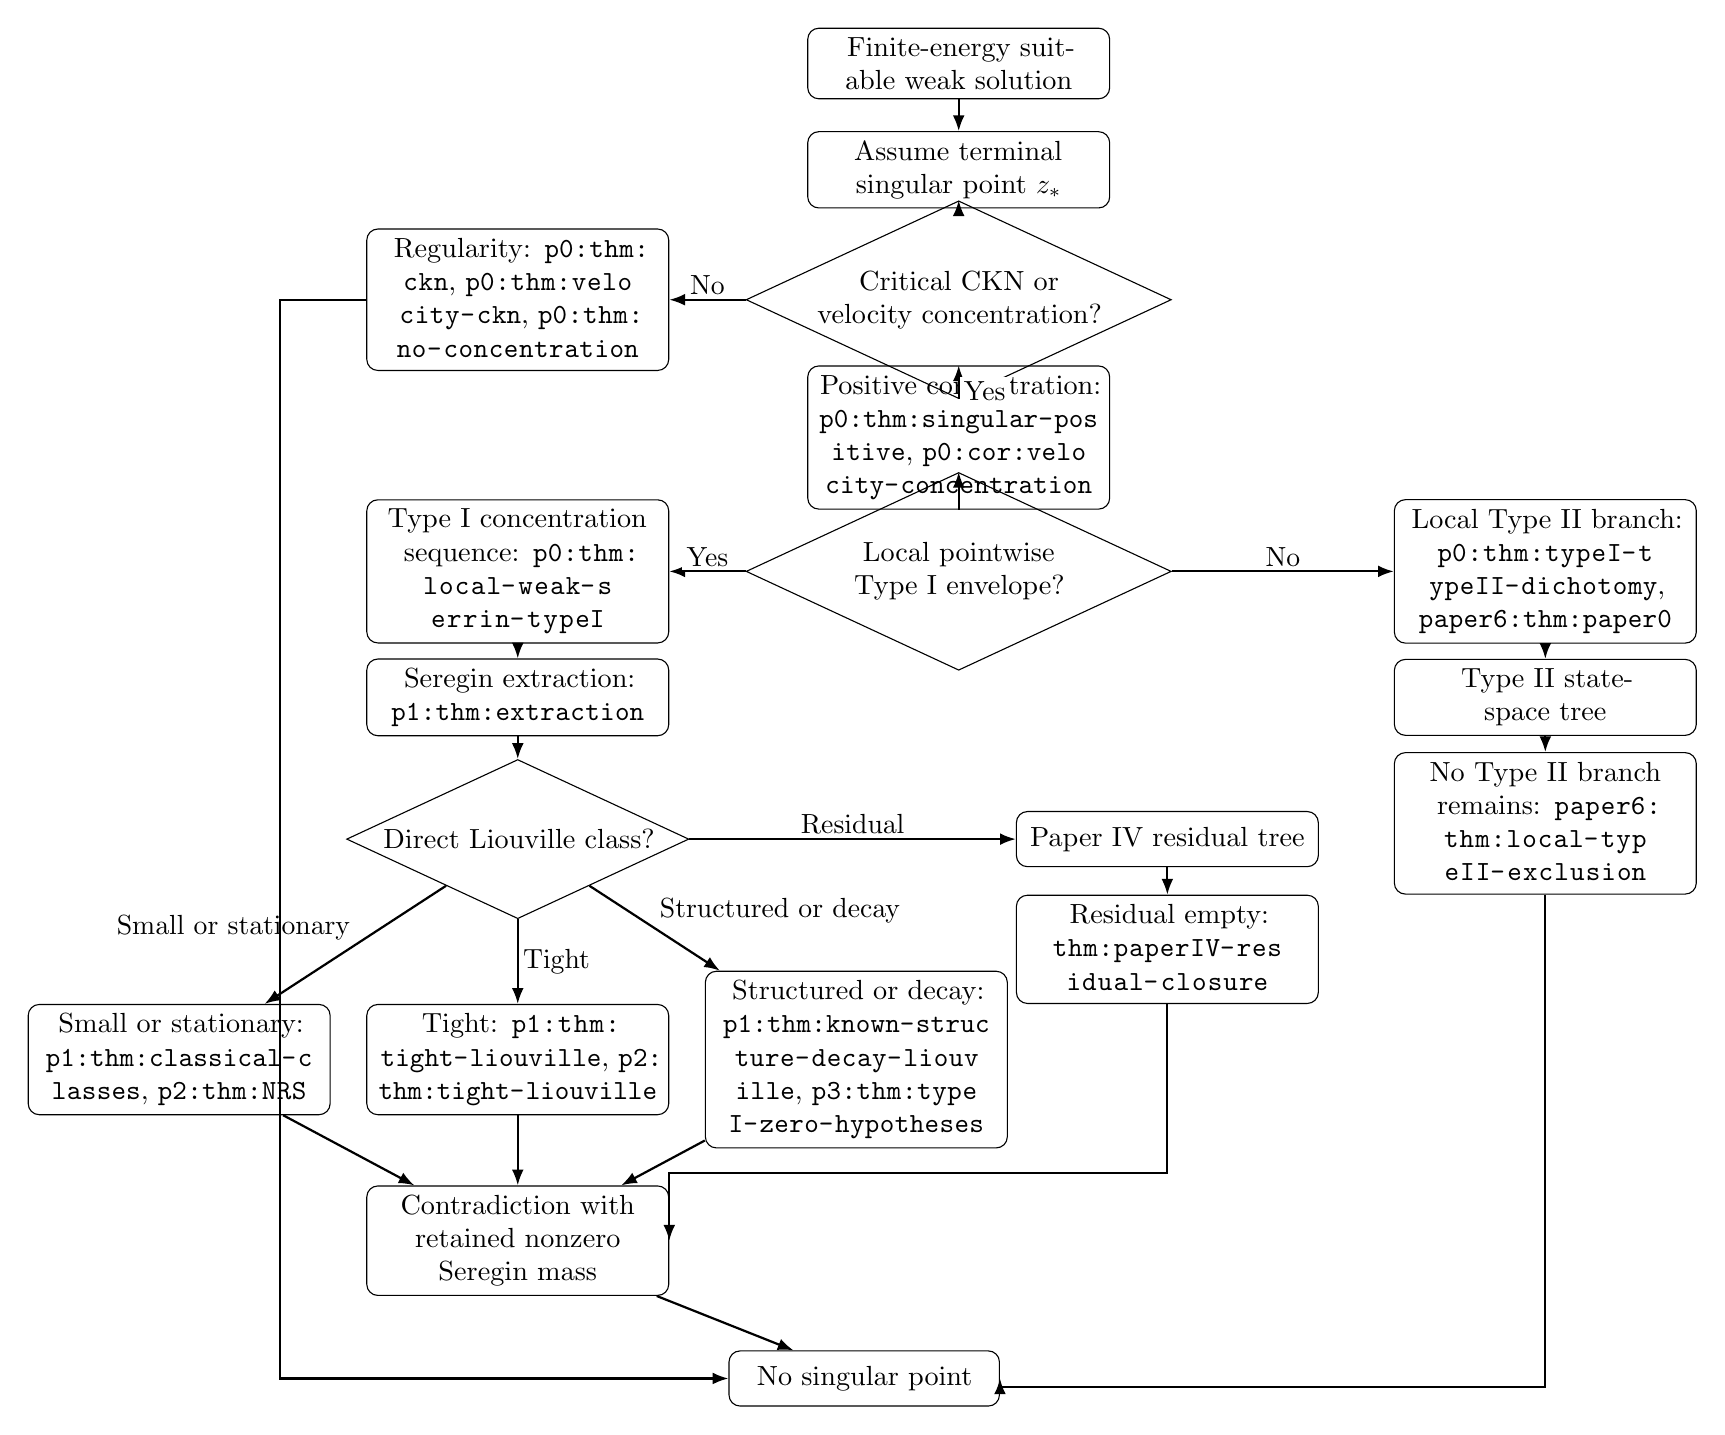
\begin{tikzpicture}[
  archnode/.style={draw, rounded corners, align=center, text width=36mm, minimum height=7mm},
  decision/.style={draw, diamond, aspect=2.15, align=center, text width=36mm, inner sep=1pt},
  arr/.style={-{Latex[length=2mm]}, thick},
  edgelabel/.style={fill=white, inner sep=1.5pt}
]
\node[archnode] (A) at (0,0) {Finite-energy suitable weak solution};
\node[archnode] (B) at (0,-1.35) {Assume terminal singular point $z_*$};
\node[decision] (C) at (0,-3.0) {Critical CKN or velocity concentration?};
\node[archnode] (C0) at (-5.6,-3.0) {Regularity: \path|p0:thm:ckn|, \path|p0:thm:velocity-ckn|, \path|p0:thm:no-concentration|};
\node[archnode] (C1) at (0,-4.75) {Positive concentration: \path|p0:thm:singular-positive|, \path|p0:cor:velocity-concentration|};
\node[decision] (D) at (0,-6.45) {Local pointwise Type I envelope?};
\node[archnode] (I0) at (-5.6,-6.45) {Type I concentration sequence: \path|p0:thm:local-weak-serrin-typeI|};
\node[archnode] (II0) at (7.45,-6.45) {Local Type II branch: \path|p0:thm:typeI-typeII-dichotomy|, \path|paper6:thm:paper0|};
\node[archnode] (I1) at (-5.6,-8.05) {Seregin extraction: \path|p1:thm:extraction|};
\node[decision] (I2) at (-5.6,-9.85) {Direct Liouville class?};
\node[archnode] (I3) at (-9.9,-12.65) {Small or stationary: \path|p1:thm:classical-classes|, \path|p2:thm:NRS|};
\node[archnode] (I4) at (-5.6,-12.65) {Tight: \path|p1:thm:tight-liouville|, \path|p2:thm:tight-liouville|};
\node[archnode] (I5) at (-1.3,-12.65) {Structured or decay: \path|p1:thm:known-structure-decay-liouville|, \path|p3:thm:typeI-zero-hypotheses|};
\node[archnode] (R0) at (2.65,-9.85) {Paper IV residual tree};
\node[archnode] (RX) at (2.65,-11.25) {Residual empty: \path|thm:paperIV-residual-closure|};
\node[archnode] (IX) at (-5.6,-14.95) {Contradiction with retained nonzero Seregin mass};
\node[archnode] (T0) at (7.45,-8.05) {Type II state-space tree};
\node[archnode] (TX) at (7.45,-9.65) {No Type II branch remains: \path|paper6:thm:local-typeII-exclusion|};
\node[archnode, text width=32mm] (END) at (-1.2,-16.7) {No singular point};
\draw[arr] (A)--(B);
\draw[arr] (B)--(C);
\draw[arr] (C)--node[edgelabel, above]{No}(C0);
\draw[arr] (C)--node[edgelabel, pos=.25, right]{Yes}(C1);
\draw[arr] (C1)--(D);
\draw[arr] (D)--node[edgelabel, above]{Yes}(I0);
\draw[arr] (D)--node[edgelabel, above]{No}(II0);
\draw[arr] (I0)--(I1);
\draw[arr] (I1)--(I2);
\draw[arr] (I2)--node[edgelabel, above left]{Small or stationary}(I3);
\draw[arr] (I2)--node[edgelabel, right]{Tight}(I4);
\draw[arr] (I2)--node[edgelabel, above right]{Structured or decay}(I5);
\draw[arr] (I2)--node[edgelabel, above]{Residual}(R0);
\draw[arr] (I3)--(IX);
\draw[arr] (I4)--(IX);
\draw[arr] (I5)--(IX);
\draw[arr] (R0)--(RX);
\draw[arr] (RX.south)--++(0,-2.15)-|(IX.east);
\draw[arr] (II0)--(T0);
\draw[arr] (T0)--(TX);
\draw[arr] (C0.west)--++(-1.1,0)|-(END.west);
\draw[arr] (IX)--(END);
\draw[arr] (TX.south)--++(0,-6.25)-|(END.east);
\end{tikzpicture}
\end{adjustbox}
\caption{Global singularity routing.}
\end{figure}
\end{landscape}

\subsection{Type I Residual Decision Tree}

\begin{landscape}
\begin{figure}[p]
\centering
\scriptsize
\begin{adjustbox}{max width=\linewidth,max totalheight=.82\textheight,center}
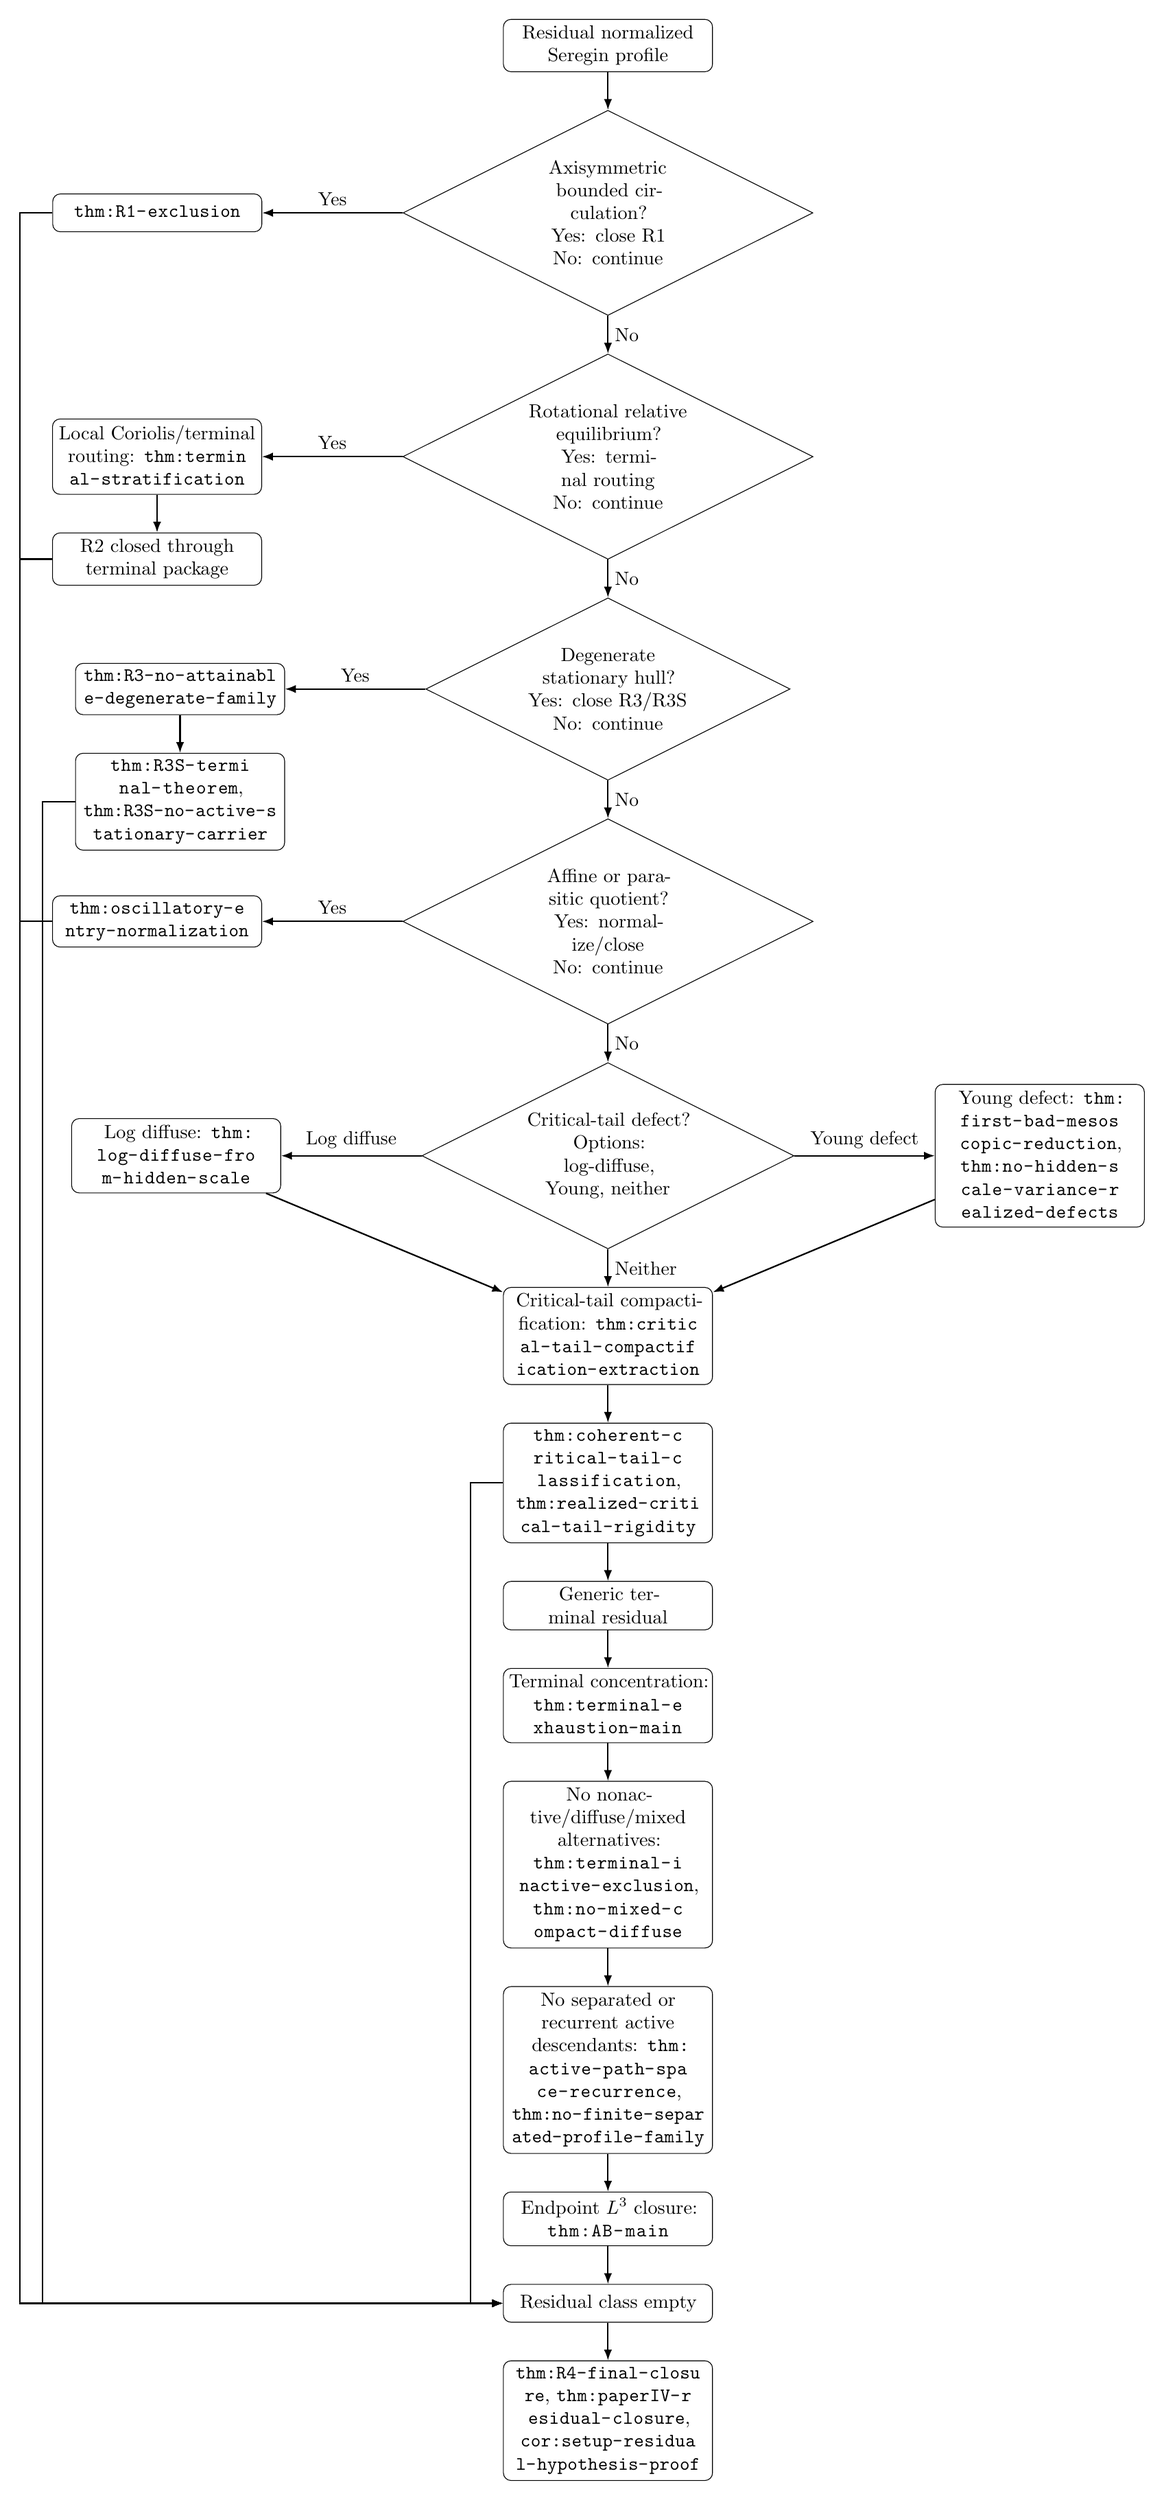
\begin{tikzpicture}[archnode/.style={draw, rounded corners, align=center, text width=0.30\textwidth, minimum height=7mm}, decision/.style={draw, diamond, aspect=2, align=center, text width=0.25\textwidth}, arr/.style={-{Latex[length=2mm]}, thick}, node distance=7mm and 9mm]
\node[archnode] (R) {Residual normalized Seregin profile};
\node[decision, below=of R] (R1) {Axisymmetric bounded circulation?\\ Yes: close R1\\ No: continue};
\node[archnode, left=of R1, xshift=-17mm] (R1x) {\path|thm:R1-exclusion|};
\node[decision, below=of R1] (R2) {Rotational relative equilibrium?\\ Yes: terminal routing\\ No: continue};
\node[archnode, left=of R2, xshift=-17mm] (R2a) {Local Coriolis/terminal routing: \path|thm:terminal-stratification|};
\node[archnode, below=of R2a] (R2x) {R2 closed through terminal package};
\node[decision, below=of R2] (R3) {Degenerate stationary hull?\\ Yes: close R3/R3S\\ No: continue};
\node[archnode, left=of R3, xshift=-17mm] (R3a) {\path|thm:R3-no-attainable-degenerate-family|};
\node[archnode, below=of R3a] (R3b) {\path|thm:R3S-terminal-theorem|, \path|thm:R3S-no-active-stationary-carrier|};
\node[decision, below=of R3] (R4) {Affine or parasitic quotient?\\ Yes: normalize/close\\ No: continue};
\node[archnode, left=of R4, xshift=-17mm] (R4x) {\path|thm:oscillatory-entry-normalization|};
\node[decision, below=of R4] (R5) {Critical-tail defect?\\ Options: log-diffuse, Young, neither};
\node[archnode, left=of R5, xshift=-17mm] (R5a) {Log diffuse: \path|thm:log-diffuse-from-hidden-scale|};
\node[archnode, right=of R5, xshift=17mm] (R5b) {Young defect: \path|thm:first-bad-mesoscopic-reduction|, \path|thm:no-hidden-scale-variance-realized-defects|};
\node[archnode, below=of R5] (R5c) {Critical-tail compactification: \path|thm:critical-tail-compactification-extraction|};
\node[archnode, below=of R5c] (R5x) {\path|thm:coherent-critical-tail-classification|, \path|thm:realized-critical-tail-rigidity|};
\node[archnode, below=of R5x] (R6) {Generic terminal residual};
\node[archnode, below=of R6] (R6a) {Terminal concentration: \path|thm:terminal-exhaustion-main|};
\node[archnode, below=of R6a] (R6b) {No nonactive/diffuse/mixed alternatives: \path|thm:terminal-inactive-exclusion|, \path|thm:no-mixed-compact-diffuse|};
\node[archnode, below=of R6b] (R6c) {No separated or recurrent active descendants: \path|thm:active-path-space-recurrence|, \path|thm:no-finite-separated-profile-family|};
\node[archnode, below=of R6c] (R6d) {Endpoint $L^3$ closure: \path|thm:AB-main|};
\node[archnode, below=of R6d] (DONE) {Residual class empty};
\node[archnode, below=of DONE] (FINAL) {\path|thm:R4-final-closure|, \path|thm:paperIV-residual-closure|, \path|cor:setup-residual-hypothesis-proof|};
\draw[arr] (R)--(R1);
\draw[arr] (R1)--node[right]{No}(R2);
\draw[arr] (R2)--node[right]{No}(R3);
\draw[arr] (R3)--node[right]{No}(R4);
\draw[arr] (R4)--node[right]{No}(R5);
\draw[arr] (R5)--node[right]{Neither}(R5c);
\foreach \a/\b in {R5c/R5x,R5x/R6,R6/R6a,R6a/R6b,R6b/R6c,R6c/R6d,R6d/DONE,DONE/FINAL}{\draw[arr] (\a)--(\b);}
\draw[arr] (R1)--node[above]{Yes}(R1x); \draw[arr] (R2)--node[above]{Yes}(R2a); \draw[arr] (R2a)--(R2x); \draw[arr] (R3)--node[above]{Yes}(R3a); \draw[arr] (R3a)--(R3b); \draw[arr] (R4)--node[above]{Yes}(R4x); \draw[arr] (R5)--node[above]{Log diffuse}(R5a); \draw[arr] (R5)--node[above]{Young defect}(R5b); \draw[arr] (R5a)--(R5c); \draw[arr] (R5b)--(R5c);
\foreach \x in {R1x,R2x,R3b,R4x,R5x}{\draw[arr] (\x.west) -- ++(-6mm,0) |- (DONE.west);}
\end{tikzpicture}
\end{adjustbox}
\caption{Type I residual decision tree.}
\end{figure}
\end{landscape}

\subsection{Paper IV Residual Branch Detailed Tree}

The expanded residual branch matches the internal organization of \path|paperIV_residual_branch.tex|.  The residual class is routed through lower strata, tail-defect compactification, terminal concentration, descendant heredity, and endpoint \(L^3\) closure.

\begin{landscape}
\begin{figure}[p]
\centering
\scriptsize
\begin{adjustbox}{max width=\linewidth,max totalheight=.82\textheight,center}
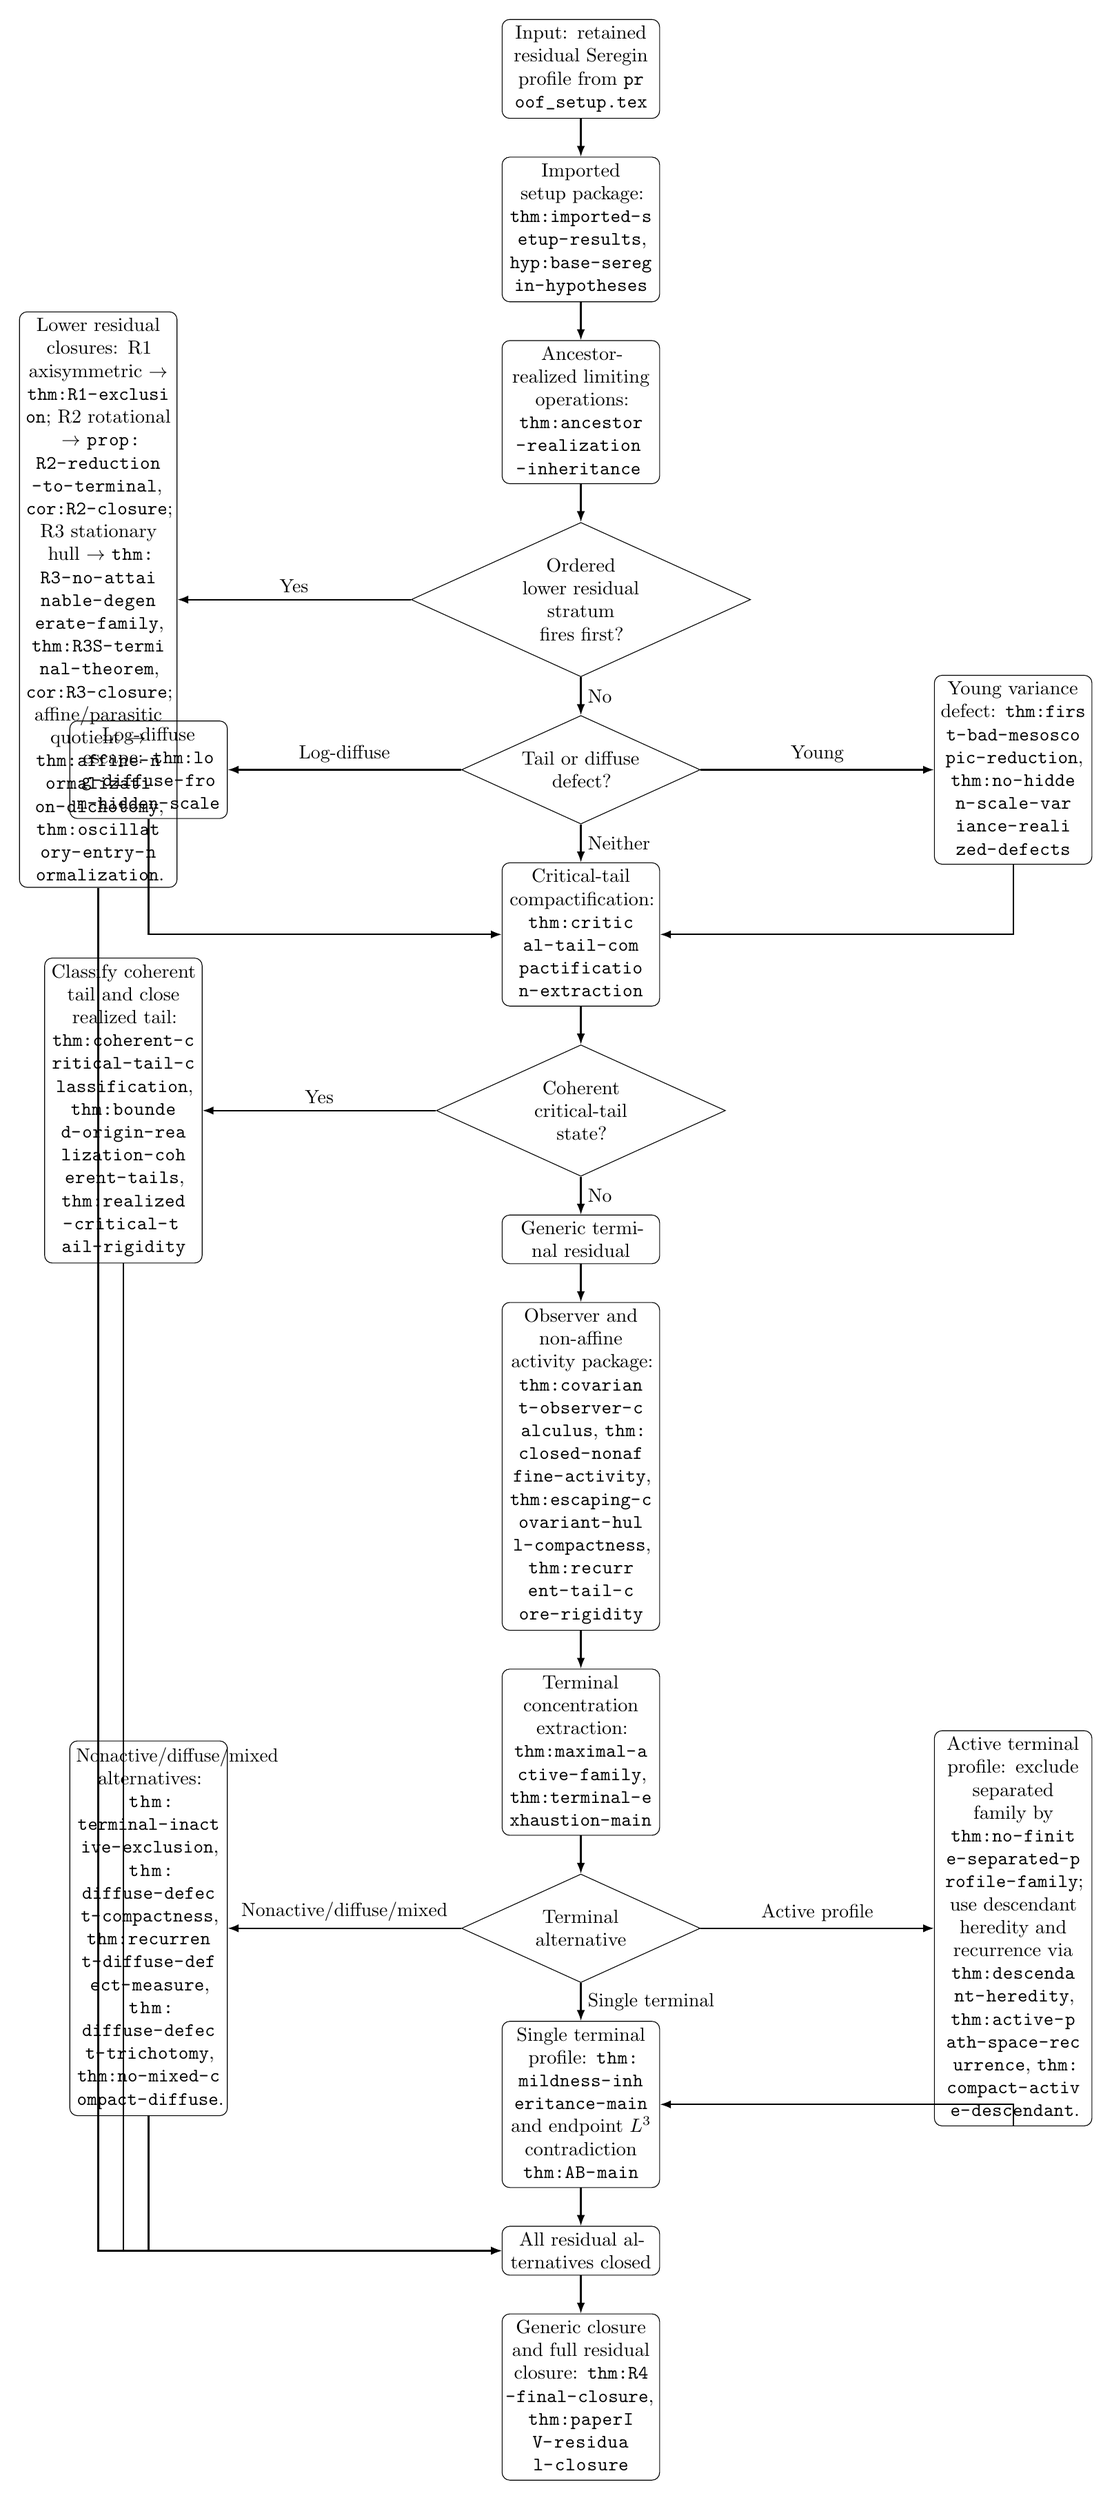
\begin{tikzpicture}[archnode/.style={draw, rounded corners, align=center, text width=0.22\linewidth, minimum height=7mm}, decision/.style={draw, diamond, aspect=2.2, align=center, text width=0.18\linewidth}, arr/.style={-{Latex[length=2mm]}, thick}, node distance=7mm and 8mm]
\node[archnode] (A) {Input: retained residual Seregin profile from \path|proof_setup.tex|};
\node[archnode, below=of A] (B) {Imported setup package: \path|thm:imported-setup-results|, \path|hyp:base-seregin-hypotheses|};
\node[archnode, below=of B] (C) {Ancestor-realized limiting operations: \path|thm:ancestor-realization-inheritance|};
\node[decision, below=of C] (D) {Ordered lower residual stratum fires first?};
\node[archnode, left=of D, xshift=-35mm] (LOW) {Lower residual closures: R1 axisymmetric \(\to\) \path|thm:R1-exclusion|; R2 rotational \(\to\) \path|prop:R2-reduction-to-terminal|, \path|cor:R2-closure|; R3 stationary hull \(\to\) \path|thm:R3-no-attainable-degenerate-family|, \path|thm:R3S-terminal-theorem|, \path|cor:R3-closure|; affine/parasitic quotient \(\to\) \path|thm:affine-normalization-dichotomy|, \path|thm:oscillatory-entry-normalization|.};
\node[decision, below=of D] (TAIL) {Tail or diffuse defect?};
\node[archnode, left=of TAIL, xshift=-35mm] (L1) {Log-diffuse escape: \path|thm:log-diffuse-from-hidden-scale|};
\node[archnode, right=of TAIL, xshift=35mm] (Y1) {Young variance defect: \path|thm:first-bad-mesoscopic-reduction|, \path|thm:no-hidden-scale-variance-realized-defects|};
\node[archnode, below=of TAIL] (CT) {Critical-tail compactification: \path|thm:critical-tail-compactification-extraction|};
\node[decision, below=of CT] (CT2) {Coherent critical-tail state?};
\node[archnode, left=of CT2, xshift=-35mm] (CT3) {Classify coherent tail and close realized tail: \path|thm:coherent-critical-tail-classification|, \path|thm:bounded-origin-realization-coherent-tails|, \path|thm:realized-critical-tail-rigidity|};
\node[archnode, below=of CT2] (GEN) {Generic terminal residual};
\node[archnode, below=of GEN] (G0) {Observer and non-affine activity package: \path|thm:covariant-observer-calculus|, \path|thm:closed-nonaffine-activity|, \path|thm:escaping-covariant-hull-compactness|, \path|thm:recurrent-tail-core-rigidity|};
\node[archnode, below=of G0] (TC) {Terminal concentration extraction: \path|thm:maximal-active-family|, \path|thm:terminal-exhaustion-main|};
\node[decision, below=of TC] (TC1) {Terminal alternative};
\node[archnode, left=of TC1, xshift=-35mm] (NON) {Nonactive/diffuse/mixed alternatives: \path|thm:terminal-inactive-exclusion|, \path|thm:diffuse-defect-compactness|, \path|thm:recurrent-diffuse-defect-measure|, \path|thm:diffuse-defect-trichotomy|, \path|thm:no-mixed-compact-diffuse|.};
\node[archnode, right=of TC1, xshift=35mm] (ACT) {Active terminal profile: exclude separated family by \path|thm:no-finite-separated-profile-family|; use descendant heredity and recurrence via \path|thm:descendant-heredity|, \path|thm:active-path-space-recurrence|, \path|thm:compact-active-descendant|.};
\node[archnode, below=of TC1] (AB) {Single terminal profile: \path|thm:mildness-inheritance-main| and endpoint $L^3$ contradiction \path|thm:AB-main|};
\node[archnode, below=of AB] (CLOSE) {All residual alternatives closed};
\node[archnode, below=of CLOSE] (FINALR) {Generic closure and full residual closure: \path|thm:R4-final-closure|, \path|thm:paperIV-residual-closure|};
\foreach \a/\b in {A/B,B/C,CLOSE/FINALR}{\draw[arr] (\a)--(\b);}
\draw[arr] (C)--(D);
\draw[arr] (D)--node[right]{No}(TAIL);
\draw[arr] (TAIL)--node[right]{Neither}(CT);
\draw[arr] (CT)--(CT2);
\draw[arr] (CT2)--node[right]{No}(GEN);
\foreach \a/\b in {GEN/G0,G0/TC,TC/TC1,AB/CLOSE}{\draw[arr] (\a)--(\b);}
\draw[arr] (D)--node[above]{Yes}(LOW); \draw[arr] (LOW)|-(CLOSE); \draw[arr] (TAIL)--node[above]{Log-diffuse}(L1); \draw[arr] (TAIL)--node[above]{Young}(Y1); \draw[arr] (L1)|-(CT); \draw[arr] (Y1)|-(CT); \draw[arr] (CT2)--node[above]{Yes}(CT3); \draw[arr] (CT3)|-(CLOSE); \draw[arr] (TC1)--node[above]{Nonactive/diffuse/mixed}(NON); \draw[arr] (NON)|-(CLOSE); \draw[arr] (TC1)--node[above]{Active profile}(ACT); \draw[arr] (ACT)|-(AB); \draw[arr] (TC1)--node[right]{Single terminal}(AB);
\end{tikzpicture}
\end{adjustbox}
\caption{Expanded Paper IV residual branch tree.}
\end{figure}
\end{landscape}

\subsection{Type II State-Space Decision Tree}
\begin{landscape}
\begin{figure}[p]
\centering
\scriptsize
\begin{adjustbox}{max width=\linewidth,max totalheight=.82\textheight,center}
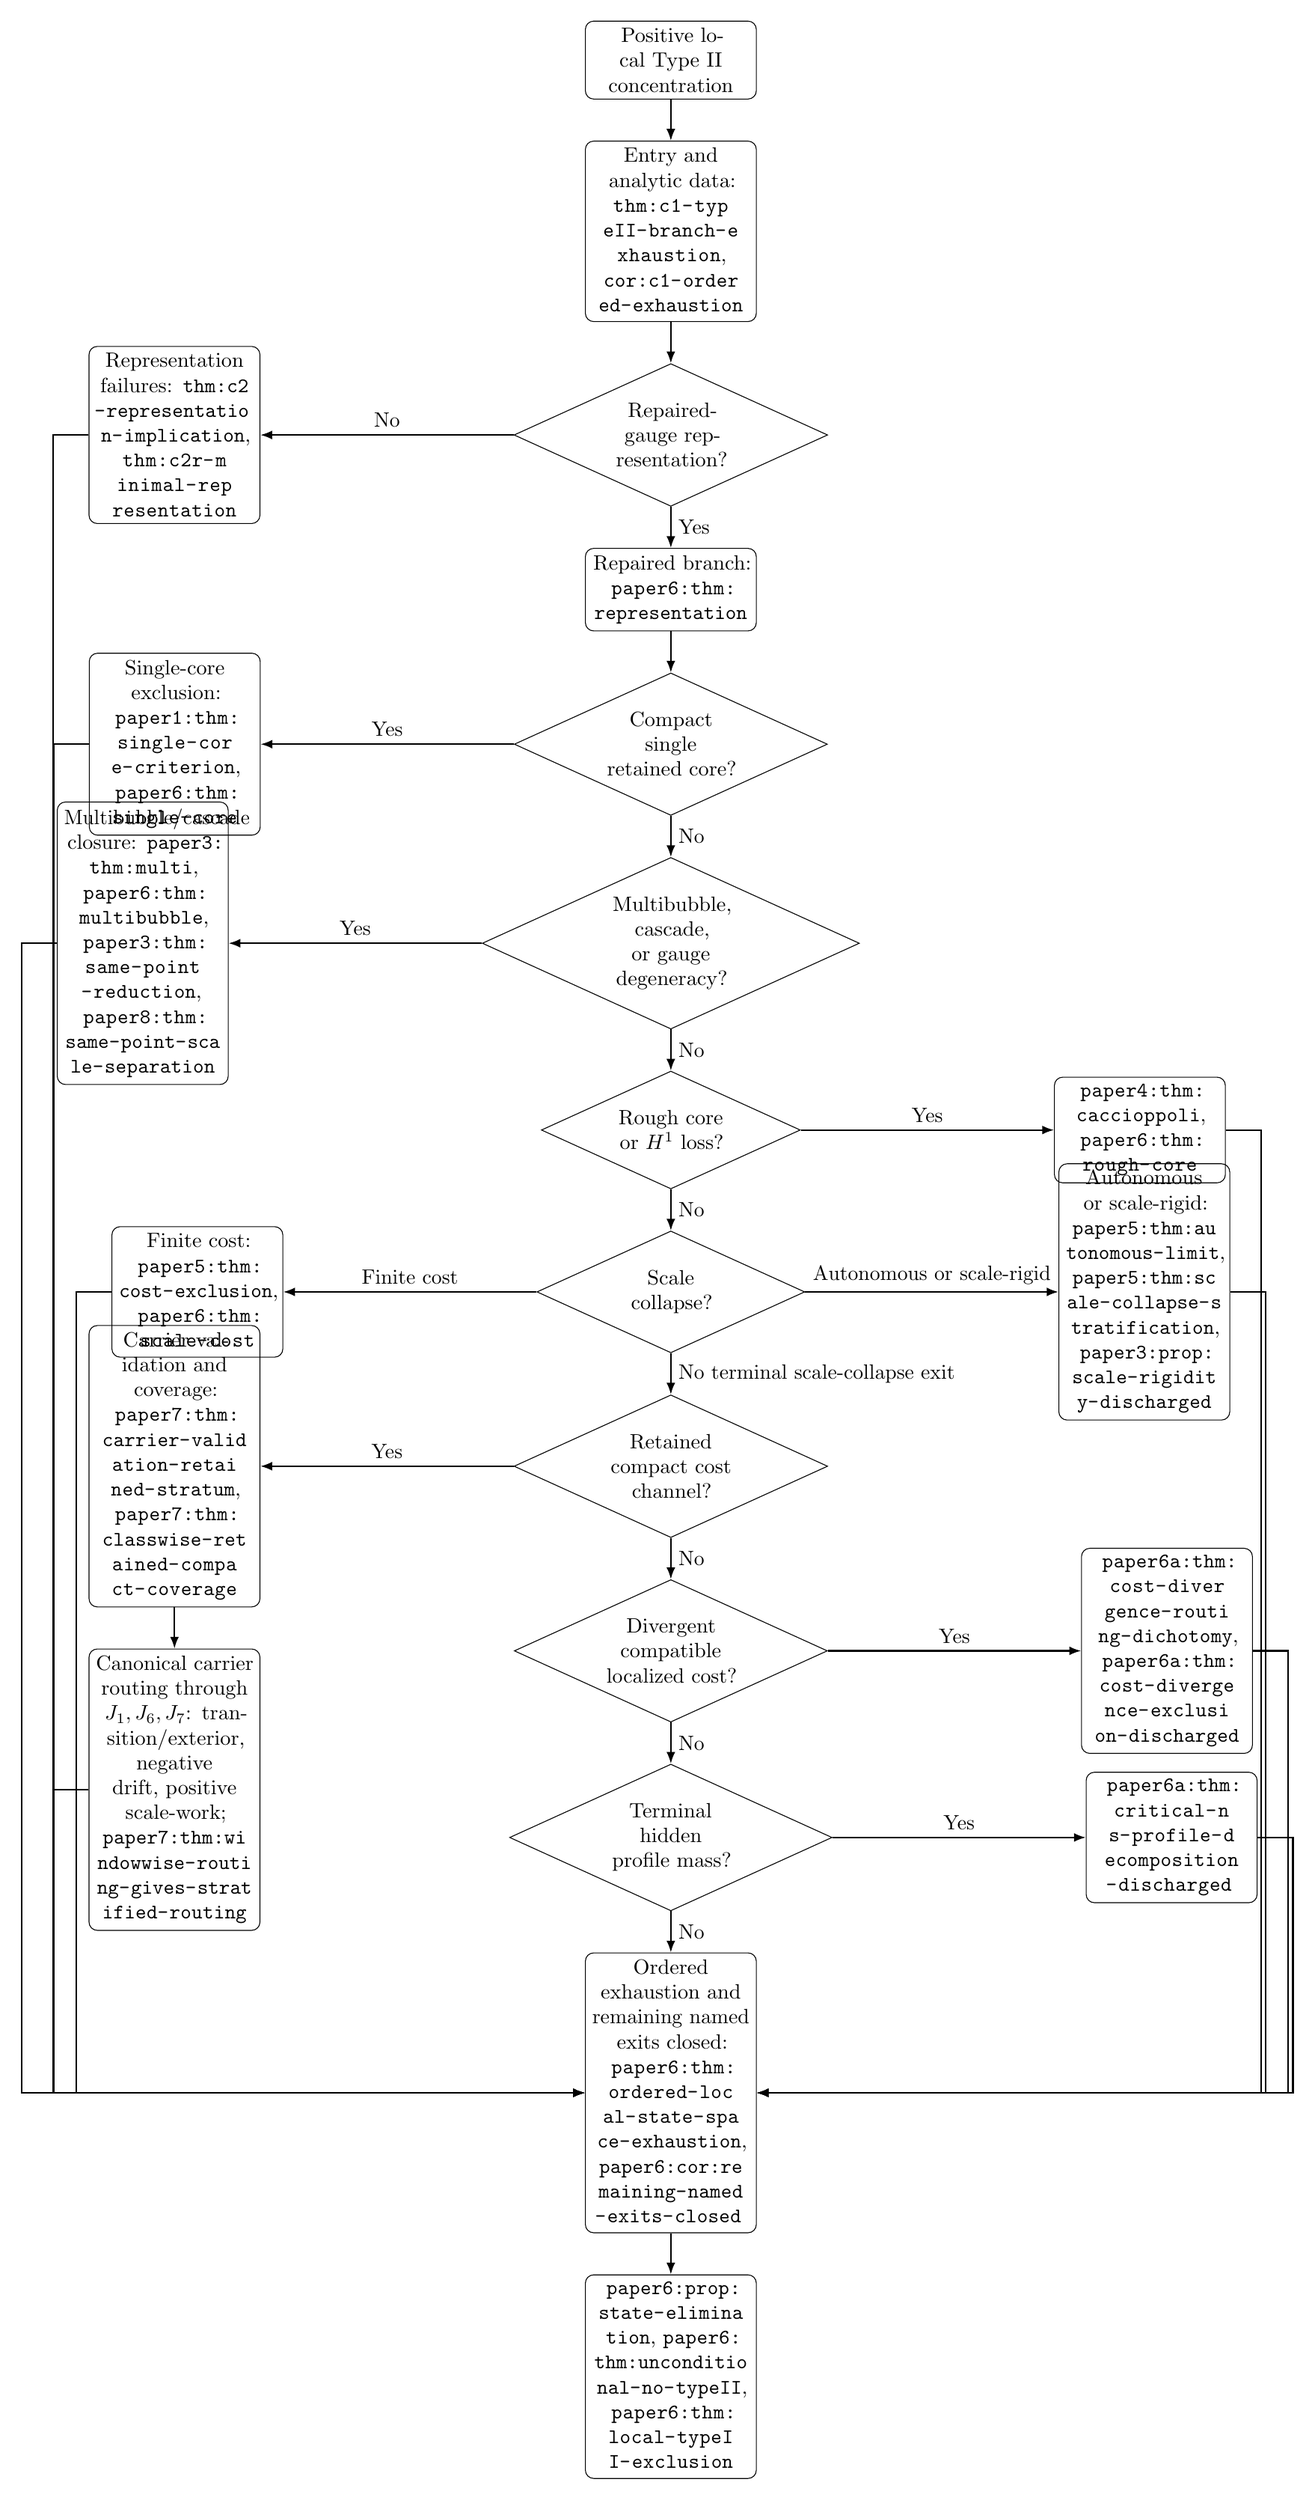
\begin{tikzpicture}[archnode/.style={draw, rounded corners, align=center, text width=0.22\linewidth, minimum height=7mm}, decision/.style={draw, diamond, aspect=2.2, align=center, text width=0.18\linewidth}, arr/.style={-{Latex[length=2mm]}, thick}, node distance=7mm and 8mm]
\node[archnode] (T) {Positive local Type II concentration};
\node[archnode, below=of T] (T1) {Entry and analytic data: \path|thm:c1-typeII-branch-exhaustion|, \path|cor:c1-ordered-exhaustion|};
\node[decision, below=of T1] (T2) {Repaired-gauge representation?};
\node[archnode, left=of T2, xshift=-35mm] (T2x) {Representation failures: \path|thm:c2-representation-implication|, \path|thm:c2r-minimal-representation|};
\node[archnode, below=of T2] (T3) {Repaired branch: \path|paper6:thm:representation|};
\node[decision, below=of T3] (T4) {Compact single retained core?};
\node[archnode, left=of T4, xshift=-35mm] (T4x) {Single-core exclusion: \path|paper1:thm:single-core-criterion|, \path|paper6:thm:single-core|};
\node[decision, below=of T4] (T5) {Multibubble, cascade, or gauge degeneracy?};
\node[archnode, left=of T5, xshift=-35mm] (T5x) {Multibubble/cascade closure: \path|paper3:thm:multi|, \path|paper6:thm:multibubble|, \path|paper3:thm:same-point-reduction|, \path|paper8:thm:same-point-scale-separation|};
\node[decision, below=of T5] (T6) {Rough core or $H^1$ loss?};
\node[archnode, right=of T6, xshift=35mm] (T6x) {\path|paper4:thm:caccioppoli|, \path|paper6:thm:rough-core|};
\node[decision, below=of T6] (T7) {Scale collapse?};
\node[archnode, left=of T7, xshift=-35mm] (T7a) {Finite cost: \path|paper5:thm:cost-exclusion|, \path|paper6:thm:scale-cost|};
\node[archnode, right=of T7, xshift=35mm] (T7c) {Autonomous or scale-rigid: \path|paper5:thm:autonomous-limit|, \path|paper5:thm:scale-collapse-stratification|, \path|paper3:prop:scale-rigidity-discharged|};
\node[decision, below=of T7] (T8) {Retained compact cost channel?};
\node[archnode, left=of T8, xshift=-35mm] (T8a) {Carrier validation and coverage: \path|paper7:thm:carrier-validation-retained-stratum|, \path|paper7:thm:classwise-retained-compact-coverage|};
\node[archnode, below=of T8a] (T9x) {Canonical carrier routing through $J_1,J_6,J_7$: transition/exterior, negative drift, positive scale-work; \path|paper7:thm:windowwise-routing-gives-stratified-routing|};
\node[decision, below=of T8] (T10) {Divergent compatible localized cost?};
\node[archnode, right=of T10, xshift=35mm] (T10x) {\path|paper6a:thm:cost-divergence-routing-dichotomy|, \path|paper6a:thm:cost-divergence-exclusion-discharged|};
\node[decision, below=of T10] (T11) {Terminal hidden profile mass?};
\node[archnode, right=of T11, xshift=35mm] (T11x) {\path|paper6a:thm:critical-ns-profile-decomposition-discharged|};
\node[archnode, below=of T11] (CLOSED) {Ordered exhaustion and remaining named exits closed: \path|paper6:thm:ordered-local-state-space-exhaustion|, \path|paper6:cor:remaining-named-exits-closed|};
\node[archnode, below=of CLOSED] (FINALII) {\path|paper6:prop:state-elimination|, \path|paper6:thm:unconditional-no-typeII|, \path|paper6:thm:local-typeII-exclusion|};
\foreach \a/\b in {T/T1,T1/T2,T3/T4,CLOSED/FINALII}{\draw[arr] (\a)--(\b);}
\draw[arr] (T2)--node[right]{Yes}(T3);
\draw[arr] (T4)--node[right]{No}(T5);
\draw[arr] (T5)--node[right]{No}(T6);
\draw[arr] (T6)--node[right]{No}(T7);
\draw[arr] (T7)--node[right]{No terminal scale-collapse exit}(T8);
\draw[arr] (T8)--node[right]{No}(T10);
\draw[arr] (T10)--node[right]{No}(T11);
\draw[arr] (T11)--node[right]{No}(CLOSED);
\foreach \x in {T2x,T4x,T5x,T7a,T9x}{\draw[arr] (\x.west) -- ++(-6mm,0) |- (CLOSED.west);}
\foreach \x in {T6x,T7c,T10x,T11x}{\draw[arr] (\x.east) -- ++(6mm,0) |- (CLOSED.east);}
\draw[arr] (T2)--node[above]{No}(T2x); \draw[arr] (T4)--node[above]{Yes}(T4x); \draw[arr] (T5)--node[above]{Yes}(T5x); \draw[arr] (T6)--node[above]{Yes}(T6x); \draw[arr] (T7)--node[above]{Finite cost}(T7a); \draw[arr] (T7)--node[above]{Autonomous or scale-rigid}(T7c); \draw[arr] (T8)--node[above]{Yes}(T8a); \draw[arr] (T8a)--(T9x); \draw[arr] (T10)--node[above]{Yes}(T10x); \draw[arr] (T11)--node[above]{Yes}(T11x);
\end{tikzpicture}
\end{adjustbox}
\caption{Type II state-space decision tree.}
\end{figure}
\end{landscape}

\subsection{Cost and Carrier Subtree}
\leavevmode\par

\begin{figure}[H]
\centering
\scriptsize
\begin{adjustbox}{max width=\linewidth,max totalheight=.82\textheight,center}
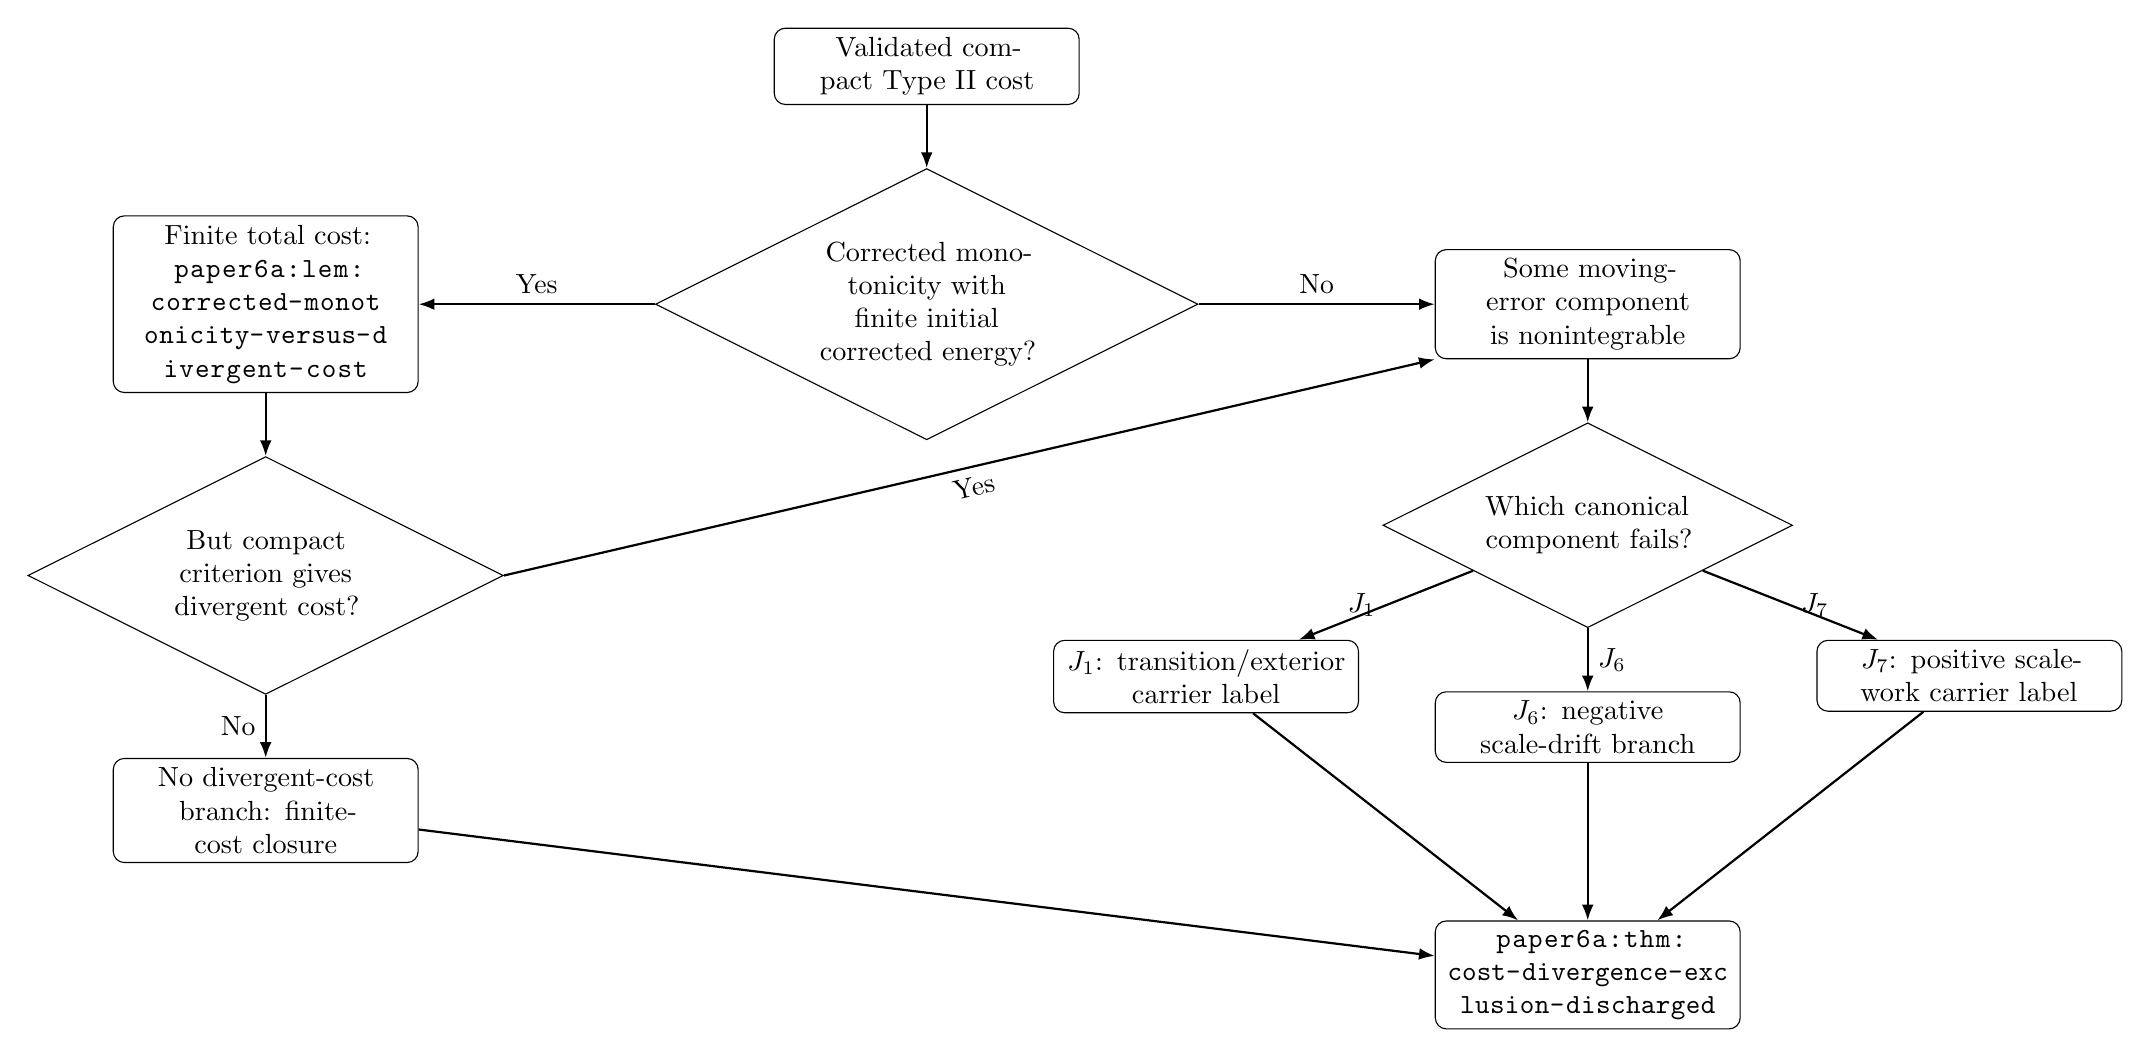
\begin{tikzpicture}[archnode/.style={draw, rounded corners, align=center, text width=0.30\textwidth, minimum height=7mm}, decision/.style={draw, diamond, aspect=2, align=center, text width=0.25\textwidth}, arr/.style={-{Latex[length=2mm]}, thick}, node distance=8mm and 10mm]
\node[archnode] (K) {Validated compact Type II cost};
\node[decision, below=of K] (K1) {Corrected monotonicity with finite initial corrected energy?};
\node[archnode, left=of K1, xshift=-20mm] (K2) {Finite total cost: \path|paper6a:lem:corrected-monotonicity-versus-divergent-cost|};
\node[archnode, right=of K1, xshift=20mm] (K3) {Some moving-error component is nonintegrable};
\node[decision, below=of K2] (K4) {But compact criterion gives divergent cost?};
\node[decision, below=of K3] (K5) {Which canonical component fails?};
\node[archnode, below=of K4] (K4n) {No divergent-cost branch: finite-cost closure};
\node[archnode, below left=of K5, xshift=-6mm] (K6) {$J_1$: transition/exterior carrier label};
\node[archnode, below=of K5] (K7) {$J_6$: negative scale-drift branch};
\node[archnode, below right=of K5, xshift=6mm] (K8) {$J_7$: positive scale-work carrier label};
\node[archnode, below=20mm of K7] (K12) {\path|paper6a:thm:cost-divergence-exclusion-discharged|};
\draw[arr] (K)--(K1); \draw[arr] (K1)--node[above]{Yes}(K2); \draw[arr] (K1)--node[above]{No}(K3); \draw[arr] (K2)--(K4); \draw[arr] (K4.east)--node[below, sloped]{Yes}(K3.south west); \draw[arr] (K4)--node[left]{No}(K4n); \draw[arr] (K3)--(K5);
\draw[arr] (K5)--node[left]{$J_1$}(K6); \draw[arr] (K5)--node[right]{$J_6$}(K7); \draw[arr] (K5)--node[right]{$J_7$}(K8); \draw[arr] (K4n)--(K12); \draw[arr] (K6)--(K12); \draw[arr] (K7)--(K12); \draw[arr] (K8)--(K12);
\end{tikzpicture}
\end{adjustbox}
\caption{Cost and carrier subtree.}
\end{figure}

\clearpage
\section{Diagram Edge Audit}

The diagrams above are theorem interfaces.  Every edge has a payload: a property that must be proved before the target node can be used.  The tables below list those properties explicitly.

\subsection{Global Routing Edges}

\begin{longtable}{@{}>{\raggedright\arraybackslash}p{0.25\linewidth}>{\raggedright\arraybackslash}p{0.35\linewidth}>{\raggedright\arraybackslash}p{0.32\linewidth}@{}}
\toprule
\textbf{Edge} & \textbf{What must be verified} & \textbf{Validation mechanism} \\
\midrule
\endhead
Finite-energy suitable weak solution to terminal singular point & The object is a suitable weak solution on a terminal time interval, with the local energy inequality and pressure normalization available. & This supplies the counterexample setup for \path|p0:thm:ckn|, \path|p0:thm:velocity-ckn|, and the local concentration package. \\
Terminal point to CKN/velocity concentration test & The CKN quantities \(C(z,r)\), \(D(z,r)\), and the velocity concentration quantity are well-defined on shrinking backward cylinders. & The first gate is scale-critical and invariant under Navier--Stokes rescaling. \\
Concentration test to regularity & Smallness must hold on a cylinder at the candidate singular point. & \path|p0:thm:ckn|, \path|p0:thm:velocity-ckn|, and \path|p0:thm:no-concentration| then give boundedness, contradicting singularity. \\
Concentration test to positive concentration & There is a sequence of shrinking cylinders carrying a fixed positive critical amount of velocity-pressure or velocity mass. & \path|p0:thm:singular-positive| and \path|p0:cor:velocity-concentration| supply the retained mass lower bound used later. \\
Positive concentration to Type I/Type II dichotomy & One must check whether a local pointwise Type I envelope holds near the terminal point. & \path|p0:thm:typeI-typeII-dichotomy| makes the split exhaustive. \\
Type I branch to Seregin extraction & The Type I envelope must give local boundedness away from \(T\), no-escape of velocity mass, local energy control, and pressure compactness. & These are the inputs to \path|p0:thm:local-weak-serrin-typeI| and \path|p1:thm:extraction|. \\
Seregin extraction to direct Liouville class test & The extracted profile must be normalized, bounded, centered, ancient, suitable, and nonzero by retained compact \(L^3\) mass. & The class tests only make sense for the normalized Seregin collection. \\
Direct Liouville class to contradiction & The relevant class hypothesis must force \(V=0\), while retained compact \(L^3\) mass remains positive. & \path|p1:thm:classical-classes|, \path|p1:thm:tight-liouville|, and \path|p1:thm:known-structure-decay-liouville| close these exits. \\
Direct class failure to residual tree & The profile must fail the small, stationary, tight, and structured/decay tests without losing normalization or retained mass. & \path|p1:thm:remaining-criterion| identifies exactly this complement as the residual class. \\
Residual tree to residual empty & The imported residual object must preserve setup ancestry, retained mass, pressure gauge, and terminal suitability through all descendant operations. & \path|thm:paperIV-residual-closure| then empties the residual class. \\
Type II branch to Type II state-space tree & The branch must carry positive concentration but no local Type I envelope, and must enter the analytic-data/exhaustion framework. & \path|paper6:thm:paper0|, \path|thm:c1-typeII-branch-exhaustion|, and \path|paper6:thm:physical-typeII-covered-entry| supply the entry. \\
Type II state-space tree to no Type II branch & Every local Type II state listed by \path|paper6:thm:state-decomposition| must be routed to a closed exit. & \path|paper6:prop:state-elimination|, \path|paper6:thm:unconditional-no-typeII|, and \path|paper6:thm:local-typeII-exclusion| finish the branch. \\
\bottomrule
\end{longtable}

\subsection{Type I Residual Edges}

\begin{longtable}{@{}>{\raggedright\arraybackslash}p{0.25\linewidth}>{\raggedright\arraybackslash}p{0.35\linewidth}>{\raggedright\arraybackslash}p{0.32\linewidth}@{}}
\toprule
\textbf{Edge} & \textbf{What must be verified} & \textbf{Validation mechanism} \\
\midrule
\endhead
Residual profile to imported setup package & The profile is the same normalized Seregin object generated by \path|proof_setup.tex|, not a newly introduced auxiliary solution. & \path|thm:imported-setup-results| and \path|hyp:base-seregin-hypotheses| fix the interface. \\
Imported setup to ancestor-realized operations & Every recentering, blow-down, hull limit, tail compactification, or terminal extraction must be sequence-realized from the original residual branch. & \path|thm:ancestor-realization-inheritance| prevents proving closure for unrelated auxiliary limits. \\
Ancestor-realized operations to ordered lower stratum & The proof must test lower residual strata in the specified order and show earlier strata are absent before later ones are used. & This prevents overlap from reintroducing already closed behavior under another name. \\
Axisymmetric residual to centered circulation closure & Axisymmetry, bounded centered angular circulation, pressure compatibility, and retained compact mass must survive the centered variables. & \path|thm:R1-exclusion| then forces a lower structured class or zero. \\
Rotational residual to terminal package & The relative-equilibrium structure must produce the local Coriolis flux identity and a terminal concentration recentering. & \path|prop:R2-reduction-to-terminal| routes the branch to terminal alternatives, and \path|cor:R2-closure| records the resulting closure after terminal stratification. \\
Degenerate stationary hull to R3S closure & The stationary-family hull element must be a sequence-realized Seregin descendant and must still carry retained concentration. & \path|thm:R3-no-attainable-degenerate-family|, \path|thm:R3S-terminal-theorem|, and \path|thm:R3S-no-active-stationary-carrier| close it. \\
Affine/parasitic quotient to oscillatory normalization & The apparent activity must be shown to be generated by affine/parasitic normalization rather than genuine nonlinear retained mass. & \path|thm:affine-normalization-dichotomy| and \path|thm:oscillatory-entry-normalization| remove that quotient. \\
Tail/diffuse defect to hidden-scale reduction & The branch must exhibit log-annular escape or Young/variance defect after compact active alternatives are absent. & \path|thm:log-diffuse-from-hidden-scale| and \path|thm:first-bad-mesoscopic-reduction| convert hidden escape into a compactified tail state or lower exit. \\
Hidden-scale branch to critical-tail compactification & The mesoscopic scales must have compactness, pressure gauges, and retained critical activity after quotienting lower affine modes. & \path|thm:critical-tail-compactification-extraction| creates the coherent-tail state space. \\
Coherent critical tail to tail rigidity & The compactified tail must be homogeneous, log-periodic, or aperiodic in the precise log-scale dynamical sense. & \path|thm:coherent-critical-tail-classification| and \path|thm:realized-critical-tail-rigidity| close realized coherent tails. \\
Generic residual to covariant observer calculus & Lower strata, affine/parasitic quotients, and coherent tails must be absent, while non-affine activity remains closed under observers. & \path|thm:covariant-observer-calculus|, \path|thm:closed-nonaffine-activity|, and \path|thm:escaping-covariant-hull-compactness| make terminal extraction legitimate. \\
Terminal concentration to terminal alternatives & Maximal active families, terminal measures, and compact/diffuse decomposition must be constructed without losing retained mass. & \path|thm:maximal-active-family| and \path|thm:terminal-exhaustion-main| make the terminal split exhaustive. \\
Terminal nonactive, diffuse, or mixed branch to closure & One must verify whether retained mass is absent, diffuse, mixed compact-diffuse, or compact active. & \path|thm:terminal-inactive-exclusion|, \path|thm:diffuse-defect-trichotomy|, and \path|thm:no-mixed-compact-diffuse| close the noncompact alternatives or reroute them. \\
Active terminal profile to descendant/separated tests & The active profile must be checked for finite separated splitting, descendant chains, recurrence, and indecomposable single-profile structure. & \path|thm:no-finite-separated-profile-family|, \path|thm:descendant-heredity|, and \path|thm:active-path-space-recurrence| remove non-single alternatives. \\
Single terminal profile to endpoint \(L^3\) closure & Parasitic-free mildness and sequence-\(L^3\) completeness must be manufactured from the preceding exclusions. & \path|thm:mildness-inheritance-main| and \path|thm:AB-main| force zero, contradicting retained mass. \\
\bottomrule
\end{longtable}

\subsection{Type II Edges}

\begin{longtable}{@{}>{\raggedright\arraybackslash}p{0.25\linewidth}>{\raggedright\arraybackslash}p{0.35\linewidth}>{\raggedright\arraybackslash}p{0.32\linewidth}@{}}
\toprule
\textbf{Edge} & \textbf{What must be verified} & \textbf{Validation mechanism} \\
\midrule
\endhead
Positive Type II concentration to analytic data & The branch must retain critical mass, local energy, pressure control, scale-window data, and the failure of every local Type I envelope. & \path|thm:c1-typeII-branch-exhaustion|, \path|cor:c1-ordered-exhaustion|, and \path|paper6a:thm:typeII-analytic-data-exhaustive| produce the analytic entry package. \\
Analytic data to repaired-gauge representation & A nondegenerate core, scale, center, time parametrization, pressure gauge, and modulation coefficients must be selected. & \path|paper6:thm:representation|, \path|thm:c2-representation-implication|, and \path|thm:c2r-minimal-representation| give the modulated local PDE. \\
Representation failure to multibubble/cascade/scale-rigid exits & If the chart is nonunique or unstable, one must identify the competing cores, scales, or degenerating scale-rigid structure. & Representation failure is not terminal; it is routed by \path|paper6:thm:state-decomposition|. \\
Repaired branch to compact single core & Compact-window bounds, pressure stability, retained mass, and vanishing localized dissipation must all hold. & \path|paper1:thm:single-core-criterion| and \path|paper6:thm:single-core| then contradict Type II or retained mass. \\
Repaired branch to rough-core exit & The branch must fail windowed \(H^1\) or compact-cylinder gradient control while keeping critical mass. & \path|paper4:thm:caccioppoli|, \path|paper7:thm:windowed-h1-failure-exclusion|, and \path|paper6:thm:rough-core| reroute roughness to closed compactness/multibubble exits. \\
Repaired branch to multibubble/cascade & Multiple active profiles, separated centers, same-point scale separation, or chart competition must be detected. & \path|paper3:thm:multi|, \path|paper3:thm:same-point-reduction|, \path|paper8:thm:same-point-scale-separation|, and terminal decoupling close or reroute the split. \\
Repaired branch to scale collapse & The selected scale must genuinely collapse relative to the terminal window and the retained core must persist. & Finite-cost exits are closed by \path|paper5:thm:cost-exclusion| and \path|paper6:thm:scale-cost|; nonfinite/autonomous exits continue to scale-rigid analysis. \\
Scale collapse to autonomous or scale-rigid state & Thick selected windows, modulation control, pressure stability, and bounded selected-window limits must be produced. & \path|paper5:thm:autonomous-limit|, \path|paper5:thm:scale-collapse-stratification|, and \path|paper3:prop:scale-rigidity-discharged| close the scale-rigid path. \\
Repaired branch to retained compact cost channel & The compact tests, retained local mass floor, localized cost comparison, and carrier validation data must all hold. & \path|paper7:thm:carrier-validation-retained-stratum| and \path|paper7:thm:classwise-retained-compact-coverage| place the branch in the cost/carrier subtree. \\
Compact cost channel to carrier completion & Fixed and moving cutoff errors must be decomposed into finite-error identities with no unrecorded cost leakage. & \path|paper7:thm:adjacent-closure-reduced-to-carrier-completion| and \path|paper7:thm:carrier-package-closes-precarrier| reduce the problem to canonical carrier components. \\
Carrier completion to \(J_1,J_6,J_7\) & The automatic moving terms must be summable; only transition, negative drift, or positive scale-shell work may remain nonintegrable. & \path|paper7:thm:windowwise-routing-gives-stratified-routing| makes the component list exhaustive. \\
\(J_1\) to transition/exterior routing & Nonintegrable transition or shell-leakage must produce a normalized carrier state with exterior/transition label. & \path|paper7:thm:windowwise-transition-routing-certificate| routes it to exterior or transition closure. \\
\(J_6\) to negative drift & Nonintegrable negative scale drift must be tied to the canonical moving cutoff and compatible scale-collapse cost. & \path|paper6a:thm:moving-cutoff-scale-collapse-alternative| and \path|paper6a:thm:finite-infinite-scale-negative| close the negative-drift exit. \\
\(J_7\) to positive scale-work & Nonintegrable positive scale-shell work must survive normalized carrier extraction and avoid earlier exterior/recentering/negative-drift labels. & \path|paper7:thm:positive-scale-certificate-enters-scale-rigid| and \path|paper7:thm:windowwise-positive-scale-routing-certificate| reroute it to scale-rigidity. \\
Divergent compatible cost to cost-divergence exclusion & Corrected monotonicity, finite initial corrected energy, and canonical windowwise compatibility must be checked. & \path|paper6a:thm:cost-divergence-routing-dichotomy| and \path|paper6a:thm:cost-divergence-exclusion-discharged| force a closed carrier exit. \\
Repaired branch to terminal hidden profile mass & Terminal frames must be sampled from the represented orbit and bounded in the critical \(L^3_\sigma\) framework. & \path|paper6a:thm:critical-ns-profile-decomposition-discharged| extracts all nonzero terminal profiles and rules out hidden mass. \\
Terminal profile branch to final Type II closure & Retained compact tests, terminal local compactness, expanded terminal data, and boundedness alternatives must all be discharged. & \path|paper6a:thm:retained-compact-tests-closed|, \path|paper6a:thm:expanded-terminal-typeII|, and \path|paper6:thm:local-typeII-exclusion| close the branch. \\
\bottomrule
\end{longtable}

\subsection{Cost and Carrier Subtree Edges}

\begin{longtable}{@{}>{\raggedright\arraybackslash}p{0.25\linewidth}>{\raggedright\arraybackslash}p{0.35\linewidth}>{\raggedright\arraybackslash}p{0.32\linewidth}@{}}
\toprule
\textbf{Edge} & \textbf{What must be verified} & \textbf{Validation mechanism} \\
\midrule
\endhead
Validated compact cost to corrected monotonicity & The localized cost, corrected energy, moving cutoff, and pressure/error terms must satisfy the fixed or moving monotonicity identity. & \path|paper6a:thm:fixed-corrected-monotonicity| and \path|paper6a:thm:moving-corrected-monotonicity| control the cost balance. \\
Corrected monotonicity to finite total cost & All error terms must be summable and the initial corrected energy finite. & Then a divergent compact cost contradicts the monotonicity balance. \\
Failure of finite total cost to nonintegrable component & The fixed and moving carrier decompositions must show that nonintegrability appears in one of the canonical components. & \path|paper7:thm:fixed-carrier-closure| and \path|paper7:thm:moving-carrier-closure| rule out unclassified error leakage. \\
Nonintegrable component to \(J_1,J_6,J_7\) & Components \(J_2,\dots,J_5\) must be automatic or summable on the canonical moving family. & The remaining component determines transition/exterior, negative drift, or positive scale-work routing. \\
\(J_1,J_6,J_7\) to cost-divergence closure & The selected component must retain its geometric label under normalized carrier-state extraction. & The corresponding closed exit feeds into \path|paper6a:thm:cost-divergence-exclusion-discharged|. \\
\bottomrule
\end{longtable}

\section{PDE Audit Points}

The following points identify where the architecture places the main PDE estimates and which hypotheses each estimate requires.

\begin{longtable}{@{}>{\raggedright\arraybackslash}p{0.30\linewidth}>{\raggedright\arraybackslash}p{0.64\linewidth}@{}}
\toprule
\textbf{Feature} & \textbf{PDE significance} \\
\midrule
\endhead
Local state-space stratification before rigidity & The argument avoids requiring a single all-purpose Liouville theorem for bounded ancient solutions.  It first routes a candidate into a stratum where a specific compactness, Liouville, virial, or cost mechanism has the required hypotheses. \\
Retained concentration as the invariant bookkeeping device & Positive CKN or compact \(L^3\) mass is carried through rescaling, gauge changes, terminal extraction, and descendant formation.  Every zero or vanishing conclusion is tested against this retained mass. \\
Type I residual closure by terminal dynamics & The residual Type I problem is treated as a structured state space rather than as an unspecified complement.  It is decomposed by terminal active loci, critical tails, diffuse defects, affine/parasitic quotients, and descendant recurrence until endpoint \(L^3\) Liouville becomes applicable. \\
Repaired-gauge Type II analysis & The Type II branch is analyzed in moving scale-center coordinates with explicit modulation coefficients.  Translation drift, scale drift, pressure gauges, and chart degeneracy become named alternatives instead of uncontrolled compactness errors. \\
Cost-divergence treatment of scale collapse & Genuine Type II scale collapse is not classified by postulating a limiting profile first.  Retained local mass forces divergence of a localized scale cost; corrected monotonicity and the canonical windowwise routing package convert that divergence into exclusion rather than leaving it as a primitive assumption. \\
No hidden global critical-norm assumption & The residual paper explicitly avoids assuming a global \(L^\infty_tL^3_x\) bound for the original residual profile.  Sequence-\(L^3\) control is manufactured only after lower strata and parasitic modes are removed. \\
No hidden global Coriolis--Leray theorem & Rotational relative equilibria are closed by local Coriolis flux and terminal concentration decomposition, not by invoking a whole-space Liouville theorem for all bounded rotating profiles. \\
Failure modes become alternatives & Missing pressure compactness, gauge degeneracy, rough-core loss, tail diffusion, critical-tail Young defects, noncompact terminal escape, and nonintegrable carrier components are routed into the ordered partition. \\
\bottomrule
\end{longtable}

For review purposes, the central structural issue is whether the routing theorems produce exactly the hypotheses required by the corresponding rigidity statements.  The terminal contradictions must be checked together with the exhaustiveness of the routing and the preservation of ancestry for all descendant profiles.

\section{Methodological Context}

The architecture can be evaluated at two levels.  At the proof level, every estimate, compactness passage, pressure reconstruction, and Liouville invocation must be correct for the three-dimensional Navier--Stokes equations.  At the methodological level, the document records a reusable audit pattern for scale-critical regularity problems: identify invariant observables, route each failure mode, and apply only the rigidity theorem justified by the stratum reached.

The table below is included only as methodological context; it is not an additional input to the proof.

\begin{longtable}{@{}>{\raggedright\arraybackslash}p{0.25\linewidth}>{\raggedright\arraybackslash}p{0.35\linewidth}>{\raggedright\arraybackslash}p{0.32\linewidth}@{}}
\toprule
\textbf{Strategy-level item} & \textbf{Generality as a PDE technique} & \textbf{Equation-dependent component} \\
\midrule
\endhead
Critical concentration as the first gate & Standard in scale-critical regularity problems.  Analogues appear whenever an epsilon-regularity or small-data criterion detects regularity below a critical threshold. & Replace CKN \(C+D\) by the problem's critical Morrey, Strichartz, energy, entropy, curvature, vorticity, or defect-measure quantity. \\
Type I/Type II separation & Applicable when there is a natural self-similar blow-up rate.  It separates controlled self-similar compactness from genuinely supercritical dynamics. & The Type I norm and rate must be the one adapted to the equation: curvature for geometric flows, critical spacetime norms for dispersive equations, gradient or energy density for heat flows. \\
Blow-up extraction into ancient or eternal objects & Common in regularity problems where singularity formation is reduced to ancient solutions, tangent flows, bubbles, or profiles. & The compactness topology changes: suitable weak limits for Navier--Stokes, Brakke/tangent flows for mean curvature, concentration compactness profiles for dispersive PDE, Uhlenbeck limits for gauge theory. \\
Retained mass bookkeeping & A contradiction proof requires a nonzero quantity that survives all limits and cannot coexist with a zero/rigid conclusion. & The retained obstruction may be energy, entropy drop, curvature concentration, enstrophy, charge, topological degree, \(L^2\) mass, or a profile norm. \\
Ordered state-space stratification & Avoids assuming a global classification theorem by using conditional classifications whose hypotheses are generated by routing. & The strata must be chosen from the equation's genuine failure modes: radiation, bubbling, necks, solitons, cascades, boundary concentration, oscillation, defect measures, or symmetry reductions. \\
Classification versus closure & Decomposition and exclusion are kept as separate statements, so any pending stratum remains visible. & Another PDE can have a complete decomposition but only partial closures; the architecture still identifies exactly which closure theorem is required. \\
Failure modes as named alternatives & A failed compactness estimate, failed gauge, or failed pressure bound produces a new branch of the proof, not an implicit assumption. & The named alternatives depend on the PDE: gauge bubbling in Yang--Mills, neck regions in harmonic map heat flow, radiation channels in dispersive PDE, shock/oscillation measures in conservation laws. \\
Repaired gauges and modulation parameters & Applies to problems with symmetries or moving concentration centers. & The parameters may be translation, scale, phase, Galilean boost, rotation, gauge transform, reparametrization, or diffeomorphism.  The orthogonality conditions and modulation equations are equation-specific. \\
Pressure/gauge bookkeeping & Specific in form but general in spirit.  Any PDE with nonlocal constraints, gauge freedom, or Lagrange multipliers needs compatible normalization across limits. & Replace pressure gauges by Coulomb gauges, DeTurck gauges, harmonic coordinates, elliptic potentials, chemical potentials, or constraint multipliers. \\
Cost-divergence or monotonicity-defect arguments & Applicable when a branch can escape by scale drift or migration.  A localized cost can convert scale escape into a quantitative contradiction, provided the error terms are either summable or routed as named carrier states. & The cost may be entropy dissipation, frequency drop, Morawetz flux, monotonicity defect, action, curvature scale drift, virial defect, or modulation energy. \\
Tail compactification and critical-tail analysis & General for noncompact critical problems where mass can escape to infinity or to logarithmic scales. & The compactification variable changes: physical infinity, frequency infinity, logarithmic scale, null infinity, neck length, or renormalized time. \\
Active-locus extraction and descendant heredity & Very general for concentration compactness.  If a proof extracts secondary profiles, it must prove they are descendants of the original counterexample and still carry the retained obstruction. & The descendant relation may be profile decomposition ancestry, tangent-flow ancestry, bubble-tree ancestry, or gauge-recentered limit ancestry. \\
Endpoint rigidity after manufacturing its hypotheses & Very general.  Instead of assuming a strong global critical bound, the proof stratifies away all failures until an endpoint theorem becomes applicable.  The architecture uses this both in the Type I residual endpoint \(L^3\) closure and in the Type II critical-profile/Kato package. & The endpoint theorem may be a Liouville theorem, scattering criterion, backward uniqueness theorem, monotonicity equality case, soliton rigidity theorem, or no-neck theorem. \\
Residual class as a structured state space & The complement of known classes is refined until it has explicit geometry and explicit closure tests. & The residual geometry is problem-specific: diffuse measures, radiation, soliton trains, neck cascades, parasitic gauge modes, or weak turbulence. \\
\bottomrule
\end{longtable}

If a specific estimate in the 3D Navier--Stokes implementation fails under review, the architecture identifies which of the following has failed:

\begin{enumerate}
\item the proposed stratum is not closed by the stated tool;
\item the routing into that stratum is not exhaustive;
\item the observable used to define the stratum is not stable under the relevant compactness or gauge operation.
\end{enumerate}

These failure modes localize the required repair: strengthen the observable, split the stratum further, prove the required rigidity theorem, or record the branch as a stated remaining obstruction.

\section{State-Space Stratification Principle}

The proof does not rely on one universal Liouville theorem for every bounded ancient solution or one universal description of every possible blow-up.  Instead it uses a decision procedure.  At every stage the proof asks a scale-invariant question whose answer places the candidate singular branch into a smaller state space.

The state space is partitioned by features that are stable under the natural Navier--Stokes rescalings:

\begin{enumerate}
\item Does the candidate singular point carry critical CKN mass?
\item Does the branch satisfy a local Type I envelope, or does every local Type I envelope fail?
\item If Type I, which centered ancient Seregin class is produced?
\item If the Seregin profile is not in a known Liouville class, which residual terminal geometry does it have?
\item If Type II, does the concentration have one retained core, several cores, a cascade, a rough core, scale collapse, or a scale-rigid terminal state?
\item If the branch escapes compactness, is the escape radiative, diffuse, critical-tail, affine/parasitic, or active and recurrent?
\end{enumerate}

The purpose of this ordered classification is to use each negative result only on the stratum where its hypotheses have been produced.  For example, endpoint \(L^3\) Liouville theory is used only after the argument has converted a profile into a sequence-\(L^3\) or uniformly tight state.  The axisymmetric circulation equation is used only after the profile has been placed in the axisymmetric bounded-circulation stratum.  Repaired gauges are used only for Type II branches where the selected core has moving scale and center.  Cost identities are used only after genuine scale collapse has been selected.

The partition is ordered rather than naively disjoint.  A profile may satisfy several descriptive properties.  The proof assigns it to the first applicable closed stratum.  This prevents overlap from creating ambiguity and prevents lower-order or already-closed behavior from being reintroduced later under a different name.

The observables used for routing are PDE observables, not formal labels.

\begin{longtable}{@{}>{\raggedright\arraybackslash}p{0.25\linewidth}>{\raggedright\arraybackslash}p{0.35\linewidth}>{\raggedright\arraybackslash}p{0.32\linewidth}@{}}
\toprule
\textbf{Observable} & \textbf{What it detects} & \textbf{Where it is used} \\
\midrule
\endhead
\(C(z,r)\) and \(D(z,r)\) & Local critical velocity-pressure concentration. & First concentration gate and Type II entry. \\
Local pointwise Type I envelope & Whether parabolic rescaling gives bounded ancient compactness. & Type I/Type II dichotomy. \\
Compact local \(L^3\) nonvanishing & The retained mass lower bound that prevents Liouville zero conclusions from being harmless. & Type I Seregin limits and terminal residual states. \\
Uniform \(L^3\)-tightness or sequence-\(L^3\) control & Whether endpoint ancient Liouville theory can be applied. & Tight Type I class and final generic residual closure. \\
Stationarity, relative equilibrium, axisymmetry, circulation, swirl & Special structures that activate known or local Liouville mechanisms. & Structured Type I classes and lower residual strata. \\
Scale-center modulation \(a,b\) & Whether a Type II core is drifting, collapsing, or approaching an autonomous regime. & Repaired-gauge Type II analysis. \\
Local windowed \(H^1\) control & Whether compactness can be upgraded from critical control. & Rough-core and compact Type II branches. \\
Active loci and diffuse defect measures & Whether terminal mass is compact, separated, diffuse, or hidden between scales. & Residual Type I closure. \\
Localized scale cost & Whether scale collapse can coexist with retained mass. & Type II scale-collapse exclusion. \\
\bottomrule
\end{longtable}

\section{The First Gate: Local Concentration and the Vanishing Branch}

The first paper, \path|proof_setup.tex|, begins with the local theory around a candidate singular point.  For \(z_0=(x_0,T)\) and \(r>0\), the basic scale-invariant quantities are

\[
  C(z_0,r)=r^{-2}\int_{Q_r(z_0)} |u|^3\,dx\,dt,
\]
and

\[
  D(z_0,r)=r^{-2}\int_{T-r^2}^{T}\int_{B_r(x_0)}
  |p-(p)_{B_r(x_0)}(t)|^{3/2}\,dx\,dt.
\]
The Caffarelli--Kohn--Nirenberg epsilon-regularity theorem says that if the critical quantity \(C+D\) is sufficiently small on a backward parabolic cylinder, then the solution is locally bounded on a smaller cylinder.  Thus a true singular point cannot be invisible to these critical quantities.

This gives the first excluded singularity type.

\begin{longtable}{@{}>{\raggedright\arraybackslash}p{0.25\linewidth}>{\raggedright\arraybackslash}p{0.35\linewidth}>{\raggedright\arraybackslash}p{0.32\linewidth}@{}}
\toprule
\textbf{Candidate type} & \textbf{Meaning} & \textbf{Exclusion mechanism} \\
\midrule
\endhead
Vanishing CKN branch & At the putative singular point, the scale-invariant velocity-pressure mass tends to zero on all sufficiently small cylinders. & CKN epsilon-regularity gives local boundedness, contradicting singularity. \\
Vanishing velocity branch & The velocity-only critical quantity \(C(z_0,r)\) tends to zero along the scales relevant to the singular point. & The velocity epsilon-regularity criterion again gives local regularity. \\
\bottomrule
\end{longtable}

After this gate, every remaining singular point has positive critical mass at arbitrarily small scales.  That positive mass is the retained obstruction carried through blow-up, compactness, recentering, and terminal-profile extraction.  Whenever a branch becomes diffuse, perturbative, or apparently vanishing, the argument checks whether the retained mass has been accounted for.  If the mass cannot be accounted for, the branch is not compatible with singularity.

\section{The Second Gate: Type I Versus Type II}

Once positive local concentration is fixed, the next partition is by blow-up rate.  A terminal point is in the local pointwise Type I branch when, in some neighborhood of the point,

\[
  \operatorname*{ess\,sup}_{T-\rho^2<t<T}
  \sqrt{T-t}\,\|u(t)\|_{L^\infty(B_\rho(x_*))}<\infty .
\]
It is in the local Type II branch when positive concentration is present but no such local Type I scale-invariant bound holds.

This dichotomy is structurally necessary: the two branches have different natural compactness theories.

\begin{longtable}{@{}>{\raggedright\arraybackslash}p{0.19\linewidth}>{\raggedright\arraybackslash}p{0.25\linewidth}>{\raggedright\arraybackslash}p{0.28\linewidth}>{\raggedright\arraybackslash}p{0.20\linewidth}@{}}
\toprule
\textbf{Branch} & \textbf{Natural rescaling} & \textbf{Main compact object} & \textbf{Main obstruction} \\
\midrule
\endhead
Local pointwise Type I & Parabolic rescaling at the singular scale, followed by centered self-similar variables. & A smooth bounded ancient Seregin profile \(V(y,\tau)\). & Bounded ancient solutions require stratification before Liouville input applies. \\
Local Type II & Selected local windows around retained concentration cores, with repaired moving scale-center gauges. & A represented local branch \((V,P,a,b)\) solving a modulated Navier--Stokes equation on compact windows. & The core may split, cascade, lose compactness, become rough, or collapse in scale. \\
\bottomrule
\end{longtable}

The proof keeps these branches separate.  The Type I argument is an ancient-solution classification problem.  The Type II argument is a local concentration-geometry problem.  Treating them separately keeps each tool in the regime where it has a precise scale-invariant meaning.

\section{The Type I Branch: From a Singular Point to a Bounded Centered Ancient State}

The Type I pipeline in \path|proof_setup.tex| is:

\begin{center}
\begin{minipage}{0.92\linewidth}
\scriptsize
\begin{verbatim}
local pointwise Type I singular point
  |
  +-- positive local velocity concentration
  |
  +-- endpoint weak-Serrin / local Type I bounds
  |
  +-- terminal velocity no-escape
  |
  +-- admissible Type I bridge sequence
  |
  +-- Seregin extraction
  |
  +-- smooth bounded ancient physical profile U
  |
  +-- centered variables
  |
  +-- normalized centered ancient profile V with retained compact L^3 mass
\end{verbatim}
\end{minipage}
\end{center}

The centered variables are

\[
  y=\frac{x}{\sqrt{-t}},\qquad
  \tau=-\log(-t),\qquad
  V(y,\tau)=\sqrt{-t}\,U(x,t),
\]
and the centered equation is

\[
  \partial_\tau V-\Delta V+\frac12 y\cdot\nabla V+\frac12 V
  +(V\cdot\nabla)V+\nabla P=0,
  \qquad \nabla\cdot V=0 .
\]
The key output is a normalized limit with positive retained local mass.  In schematic terms, there are compact sets and times for which

\[
  \int_{K} |V(y,\tau)|^3\,dy > 0
\]
in the limiting profile.  This nonvanishing condition is what contradicts every Liouville conclusion \(V\equiv0\).

The pressure bookkeeping matters here.  The source pressure \(p\), the physical ancient pressure \(Q\), and the centered pressure \(P\) are all understood modulo functions of time.  This gauge freedom is harmless for the equations and the local energy inequality, but it is essential for compactness: pressure limits must be compared in compatible local gauges rather than as absolute functions.

\subsection{Role of Seregin Extraction}

Seregin extraction is used in the Type I branch because the Type I envelope produces uniform local boundedness away from the terminal time after rescaling.  It converts a dynamic singularity into an ancient object on the whole time interval \((-\infty,0)\), and centered variables turn the self-similar scaling into time translation in \(\tau\).  This reduces the branch to a classification problem for bounded ancient trajectories, where Liouville and compact-dynamical tools apply.

\subsection{The First Type I State-Space Partition}

The setup paper defines a collection \(\mathcal S\) of normalized Seregin ancient limits generated by admissible Type I extractions.  Each element \(V\in\mathcal S\) is assigned to one of the following classes:

\begin{longtable}{@{}>{\raggedright\arraybackslash}p{0.25\linewidth}>{\raggedright\arraybackslash}p{0.35\linewidth}>{\raggedright\arraybackslash}p{0.32\linewidth}@{}}
\toprule
\textbf{Type I class} & \textbf{Selection criterion} & \textbf{Closure mechanism} \\
\midrule
\endhead
Small-amplitude class & The bounded ancient profile is sufficiently small in the relevant scale-invariant topology. & Perturbative bounded ancient Liouville theory forces \(V=0\). \\
Stationary \(L^3\) class & The centered profile has a stationary representative with critical \(L^3\) control. & The Ne\v{c}as--R\r{u}\v{z}i\v{c}ka--\v{S}ver\'ak stationary self-similar rigidity theorem excludes nonzero profiles. \\
Uniformly \(L^3\)-tight class & The profile's \(L^3\) mass remains uniformly tight in space along the ancient time direction. & Physical pullback gives the endpoint sequence-\(L^3\) structure needed for the Albritton--Barker ancient Liouville theorem. \\
Liouville-covered structure/decay class & The profile has one of the explicitly listed structures or decay properties covered by known Liouville theorems. & Axisymmetric, swirl, weighted-vorticity, or other cited rigidity mechanisms force zero. \\
Remaining/residual class & The complement of the previous four classes inside \(\mathcal S\). & Not closed in the setup paper; refined and closed in \path|paperIV_residual_branch.tex|. \\
\bottomrule
\end{longtable}

The first four classes are not required to be disjoint.  The residual class is the complement of their union after those classes have been removed.  In this document, ``residual'' means not already removed by the available direct Liouville mechanisms; it does not denote an unstructured singular class.

\section{The Non-Residual Type I Tools}

The setup paper chooses tools according to the amount of structure already visible in the Seregin limit.

\begin{longtable}{@{}>{\raggedright\arraybackslash}p{0.25\linewidth}>{\raggedright\arraybackslash}p{0.35\linewidth}>{\raggedright\arraybackslash}p{0.32\linewidth}@{}}
\toprule
\textbf{Tool} & \textbf{Where it enters} & \textbf{Role in the proof} \\
\midrule
\endhead
Endpoint weak-Serrin local Type I estimate & Before Seregin extraction. & It prevents velocity mass from escaping into the terminal time slice and supplies the local energy control needed for admissibility. \\
Local compactness and pressure normalization & During blow-up extraction. & It provides a suitable ancient limit and keeps pressure meaningful modulo functions of time. \\
Centered self-similar variables & After physical ancient extraction. & They convert the Type I scaling symmetry into an autonomous centered ancient equation. \\
Perturbative Liouville theorem & Small-amplitude class. & Small bounded ancient solutions cannot carry retained concentration. \\
NRS stationary rigidity & Stationary \(L^3\) class. & A stationary finite-\(L^3\) self-similar profile must vanish. \\
Albritton--Barker endpoint ancient Liouville theorem & Uniformly \(L^3\)-tight class. & Tightness plus boundedness yields the sequence-\(L^3\) hypothesis needed to force zero. \\
Axisymmetric and weighted-vorticity Liouville mechanisms & Structured/decay class. & They exploit special geometric or weighted decay properties instead of requiring a universal ancient Liouville theorem. \\
\bottomrule
\end{longtable}

The non-residual Type I conclusion is therefore:

\begin{center}
\begin{minipage}{0.92\linewidth}
\scriptsize
\begin{verbatim}
normalized Type I Seregin profile
  |
  +-- in small/stationary/tight/structured class --> V = 0
  |
  +-- but V has retained compact L^3 mass       --> contradiction
\end{verbatim}
\end{minipage}
\end{center}

The only Type I branch left after this point is the residual branch.

\section{The Residual Type I Branch}

The residual paper, \path|paperIV_residual_branch.tex|, begins after the setup paper has removed the small, stationary \(L^3\), uniformly tight, and closed structured/decay alternatives.  A residual candidate is therefore a bounded normalized centered ancient Seregin profile with retained local concentration which has avoided all direct Liouville classes.

The residual paper treats the remaining class as a structured state space with terminal geometry.  The proof refines the residual state space by asking ordered questions about symmetry, rotation, stationary hulls, affine/parasitic modes, tail compactness, active loci, diffuse defects, and terminal recurrence.

The residual decomposition is:

\begin{center}
\begin{minipage}{0.92\linewidth}
\scriptsize
\begin{verbatim}
coarse Type I residual class
  |
  +-- axisymmetric bounded-circulation residual class C_ax
  +-- rotational relative-equilibrium class C_rot
  +-- degenerate stationary-hull class C_stat
  +-- affine/parasitic quotient stratum C_aff
  +-- log-diffuse critical-tail alternative C_logdiff
  +-- Young critical-tail alternative C_young
  +-- coherent homogeneous critical tail C_homcrit
  +-- coherent log-periodic critical tail C_logper
  +-- coherent aperiodic critical tail C_apcrit
  +-- generic terminal residual C_gen
\end{verbatim}
\end{minipage}
\end{center}

Again, this is an ordered partition.  The proof does not need the classes to be intrinsically disjoint in every possible descriptive sense.  It needs a deterministic routing rule: after earlier strata have been removed, the first remaining terminal behavior determines the next stratum.

\subsection{Residual Type I Taxonomy}

\begin{longtable}{@{}>{\raggedright\arraybackslash}p{0.25\linewidth}>{\raggedright\arraybackslash}p{0.35\linewidth}>{\raggedright\arraybackslash}p{0.32\linewidth}@{}}
\toprule
\textbf{Residual stratum} & \textbf{What it represents} & \textbf{Main closure mechanism} \\
\midrule
\endhead
\(\mathcal C_{\rm ax}\): axisymmetric bounded-circulation residual & The Seregin profile has axisymmetric geometry and bounded centered angular circulation, but was not already removed by the setup structured class. & A centered angular-circulation equation plus axis-absorption Liouville theorem forces the profile into a no-swirl/lower structured class, contradicting residuality. \\
\(\mathcal C_{\rm rot}\): rotational relative equilibrium & The profile is stationary only modulo rotation, producing a local Coriolis-type transport structure. & A localized Coriolis-flux identity and local concentration recentering show that either a lower compact profile is produced or the profile falls into an endpoint critical class already closed. No global Coriolis--Leray Liouville theorem is used. \\
\(\mathcal C_{\rm stat}\): degenerate stationary hull with retained concentration & Time-translation hulls of the ancient trajectory contain degenerate stationary-family elements that still carry local concentration. & Scale reselection and the terminal local concentration theorem rule out stationary-family concentration profiles that occur as Seregin descendants after lower classes are removed. \\
\(\mathcal C_{\rm aff}\): affine/parasitic quotient stratum & The residual behavior is an affine or parasitic mode generated by gauge normalization rather than a genuine retained nonlinear residual profile. & Oscillatory-entry normalization removes the quotient stratum: no retained normalized representative remains there. \\
\(\mathcal C_{\log\rm diff}\): log-diffuse tail & Critical activity escapes through logarithmic annuli without becoming a compact active profile. & The branch is reduced to hidden-scale compactness and the minimal mesoscopic-scale reduction theorem. \\
\(\mathcal C_{\rm Young}\): Young critical-tail alternative & Critical tail mass survives only as a Young-measure or variance defect rather than a strong local profile. & Fr\'echet--Kolmogorov/Young-measure compactness reduces the defect to the same minimal mesoscopic-scale theorem. \\
\(\mathcal C_{\rm homcrit}\): coherent homogeneous tail & The terminal tail becomes a coherent \((-1)\)-homogeneous critical profile. & Bounded-origin realization and local boundedness contradict the retained residual profile. \\
\(\mathcal C_{\log\rm per}\): coherent log-periodic tail & The tail is coherent and periodic in logarithmic scale. & The coherent critical-tail closure excludes realized log-periodic critical tails. \\
\(\mathcal C_{\rm apcrit}\): coherent aperiodic tail & The tail has a compact log-translation hull but no nonzero log period. & The aperiodic hull is closed by the same coherent critical-tail rigidity mechanism. \\
\(\mathcal C_{\rm gen}\): generic terminal residual & Everything left after all lower residual alternatives and tail alternatives have been removed. & Terminal concentration analysis, active path-space recurrence, finite separated-profile exclusion, parasitic-free mildness, sequence-\(L^3\) completeness, and the endpoint ancient Liouville theorem force zero. \\
\bottomrule
\end{longtable}

\subsection{Role of the Residual Tools}

The residual branch requires separate treatment because a direct global \(L^3\) bound or global Liouville theorem is not available at the start.  The residual paper therefore derives the needed endpoint conclusion only after eliminating the alternatives that obstruct it.

A residual profile may have local boundedness and retained compact mass while still failing every direct global critical-space hypothesis.  The proof first removes affine/parasitic modes, diffuse tails, coherent critical tails, and active descendant chains.  Only after these exits are closed does the generic residual branch inherit the mildness and sequence-\(L^3\) structure needed for the endpoint ancient Liouville theorem.

The main residual tools are:

\begin{longtable}{@{}>{\raggedright\arraybackslash}p{0.30\linewidth}>{\raggedright\arraybackslash}p{0.64\linewidth}@{}}
\toprule
\textbf{Residual tool} & \textbf{Purpose} \\
\midrule
\endhead
Ancestor-realization and heredity & Ensures that descendants produced by recentering, blow-down, or terminal extraction are still connected to the original singularity-generated profile. This prevents the proof from proving a theorem about an auxiliary object that is not inherited by the original branch. \\
Terminal local concentration theorem & Classifies where retained local mass can go after lower classes are removed. It excludes pure local vanishing, pure exterior escape, and noncompact terminal alternatives as sole carriers of the retained mass. \\
Active-locus extraction & Identifies compact regions where a fixed positive amount of critical activity persists. These regions become the nodes of the terminal state-space graph. \\
Diffuse-defect compactness & Handles residual mass that does not localize into finitely many active cores. It distinguishes active regeneration, affine/parasitic collapse, and critical diffuse tails. \\
Minimal mesoscopic-scale reduction & Prevents hidden critical-tail defects from surviving only between visible scales. It routes log-diffuse and Young alternatives into active, affine, or coherent critical-tail strata. \\
Critical-tail compactification & Converts noncompact tail behavior into a compact log-scale dynamical problem with homogeneous, log-periodic, and aperiodic alternatives. \\
Active path-space recurrence & Rules out infinite chains or loops of retained active descendants. \\
Finite separated-profile exclusion & Prevents retained concentration from splitting into a finite separated family that avoids all lower strata. \\
Parasitic-free mildness inheritance & After affine/parasitic modes are removed, the physical pullback inherits the mild bounded ancient structure needed for endpoint Liouville theory. \\
Sequence-\(L^3\) completeness & Converts terminal indecomposability into the sequence-\(L^3\) condition needed by Albritton--Barker. \\
\bottomrule
\end{longtable}

The final generic residual closure is conceptually:

\begin{center}
\begin{minipage}{0.92\linewidth}
\scriptsize
\begin{verbatim}
generic residual profile
  |
  +-- if active compact concentration remains
  |       +-- finite/infinite descendant analysis
  |       +-- recurrence and separated-family exclusions
  |
  +-- if diffuse or tail concentration remains
  |       +-- diffuse-defect trichotomy
  |       +-- mesoscopic-scale reduction
  |       +-- critical-tail closure
  |
  +-- after all lower exits are closed
          +-- profile is parasitic-free and sequence-L^3
          +-- Albritton--Barker endpoint Liouville
          +-- profile is zero
          +-- contradiction with retained local mass
\end{verbatim}
\end{minipage}
\end{center}

Thus the residual proof does not require a universal Liouville theorem for every bounded centered ancient residual profile.  It shows that any residual profile avoiding the lower strata becomes endpoint Liouville-admissible.

\section{The Type I Assembly}

Combining \path|proof_setup.tex| and \path|paperIV_residual_branch.tex|, the Type I singularity exclusion has the following structure:

\begin{longtable}{@{}>{\raggedright\arraybackslash}p{0.25\linewidth}>{\raggedright\arraybackslash}p{0.35\linewidth}>{\raggedright\arraybackslash}p{0.32\linewidth}@{}}
\toprule
\textbf{Step} & \textbf{Input} & \textbf{Output} \\
\midrule
\endhead
Local concentration & \(z_*=(x_*,T)\) singular and local pointwise Type I. & A positive local velocity concentration sequence. \\
No-escape bridge & Endpoint weak-Serrin/local Type I estimates. & The concentration sequence is admissible for Seregin extraction. \\
Seregin extraction & Admissible Type I bridge sequence. & A smooth bounded centered ancient limit \(V\) with retained compact \(L^3\) mass. \\
Setup class exhaustion & Definition of \(\mathcal S\). & \(V\) is in a non-residual Liouville class or in the residual class. \\
Non-residual closure & Perturbative, stationary, tight, and structured Liouville mechanisms. & Non-residual classes force \(V=0\), contradicting retained compact \(L^3\) mass. \\
Residual closure & Refined residual decomposition in \path|paperIV_residual_branch.tex|. & Residual class is empty, so \(V\) cannot exist. \\
\bottomrule
\end{longtable}

Thus a local pointwise Type I singularity cannot occur once the setup and residual papers are combined.

\section{The Type II Branch: Required Classification}

The Type II paper starts from the other side of the first dichotomy: positive local critical concentration is present, but no local Type I scale-invariant bound holds.  The branch is more geometric than the Type I branch because no single self-similar scale is fixed by the Type I envelope.  The concentration may move, split, collapse, or interact across scales.

The Type II paper therefore selects local windows around retained cores and uses repaired gauges.  A typical represented branch satisfies a modulated renormalized Navier--Stokes equation

\[
  \partial_\tau V+(V\cdot\nabla)V+\nabla P
  =
  \nu\Delta V+a(\tau)(V+y\cdot\nabla V)+b(\tau)\cdot\nabla V,
  \qquad \nabla\cdot V=0.
\]
Here \(a(\tau)\) records scale modulation and \(b(\tau)\) records translation modulation.  The repaired gauge chooses the scale and center so that the selected core stays in a controlled coordinate system and the modulation terms are not arbitrary gauge artifacts.

The repaired chart is designed to preserve the parabolic character of the equation: the time reparametrization is tied to the spatial scale so that the viscosity coefficient remains fixed in the renormalized equation.  Consequently, the Type II analysis can still use local energy, Caccioppoli, pressure reconstruction, and compactness estimates in the transformed variables.

\subsection{Role of Repaired Gauges}

Without a repaired gauge, a Type II concentration branch may appear noncompact because the core center moves, the selected scale drifts, or two nearby possible cores compete for the normalization.  Repaired gauges separate these effects:

\begin{longtable}{@{}>{\raggedright\arraybackslash}p{0.30\linewidth}>{\raggedright\arraybackslash}p{0.64\linewidth}@{}}
\toprule
\textbf{Problem} & \textbf{Repaired-gauge response} \\
\midrule
\endhead
Moving concentration center & Track a center \(x_c(\tau)\) and convert motion into a controlled transport term \(b(\tau)\cdot\nabla V\). \\
Changing concentration scale & Track a scale \(\lambda(\tau)\) and convert scale drift into \(a(\tau)(V+y\cdot\nabla V)\). \\
Pressure gauge ambiguity & Reconstruct pressure locally modulo functions of time, matching the local energy inequality. \\
Loss of compactness by bad coordinates & Use moment or localization constraints to pin down a canonical local chart where compactness questions are meaningful. \\
Gauge degeneracy & Route failure of the gauge into multibubble, cascade, or scale-rigidity alternatives instead of hiding it inside estimates. \\
\bottomrule
\end{longtable}

The represented Type II branch is not the conclusion of the proof.  It is the coordinate system in which the state-space partition becomes precise.

The nontrivial analytic burden is that the represented branch must remain a suitable local Navier--Stokes object after the transformation.  The pressure must be reconstructed modulo functions of time, the local energy inequality must survive on compact windows, and the modulation coefficients must be measurable or locally integrable enough for the distributional identities and compactness arguments.  These requirements explain why representation failure is itself part of the Type II partition.

\section{Type II State-Space Partition}

The Type II paper decomposes every positive local Type II concentration sequence into local alternatives and closes each exit.  The final assembly distinguishes the geometric alternatives from the local cost/carrier interfaces that close the compact-cost channel:

\begin{longtable}{@{}>{\raggedright\arraybackslash}p{0.25\linewidth}>{\raggedright\arraybackslash}p{0.35\linewidth}>{\raggedright\arraybackslash}p{0.32\linewidth}@{}}
\toprule
\textbf{Type II alternative} & \textbf{Meaning} & \textbf{Closure mechanism} \\
\midrule
\endhead
Compact single-core vanishing-dissipation branch & One retained core is selected, compact-window estimates hold, pressure is stable, modulation is bounded, and localized dissipation vanishes. & Local compactness gives a spatially constant or bounded selected-window limit. A zero limit contradicts retained concentration; a nonzero bounded selected-window limit contradicts the Type II regime. \\
Bounded selected-window and reselection rows & A bounded selected-window limit, pressure-only signal, or diffuse reselection-tree support appears before the branch has been assigned to a retained row. & The bounded-window row is physically routed by \path|paper6:thm:bounded-selected-window-physical-routing|; reselection support is well-founded by the \path|paper10| tree and cannot be an independent terminal exit. \\
Multibubble, cascade, or gauge-degenerate branch & Positive concentration splits into several active profiles, comparable-scale classes, same-point cascades, separated centers, or nonunique/gauge-degenerate core choices. & Active-profile decoupling, terminal profile decoupling, same-point cascade exclusion, separated-point reduction, and the discharged scale-rigidity package eliminate these branches. \\
Rough-core / loss of windowed \(H^1\) control & The selected core keeps critical mass but lacks the compact-cylinder gradient control needed for the compact argument. & Local Caccioppoli estimates show finite outer \(C+D\) control gives inner \(H^1\) control. Failure of \(H^1\) control is routed back to compactness failure or multibubble/cascade alternatives. \\
Finite-cost scale-collapse branch & The selected scale genuinely collapses but the scale-collapsing cost or absolute scale cost is finite. & Localized cost identities show finite cost is incompatible with a nonvanishing retained core. \\
Retained compact cost channel & The branch survives the compact-cost validation tests and carries a validated compact Type II cost-divergence conclusion. & Section 7 verifies the local cost-exclusion data on the retained stratum, proves classwise retained compact coverage, and reduces adjacent exits to the canonical carrier/routing package. \\
Windowwise carrier-routing alternatives & On the canonical moving cutoff, the only nonautomatic moving components after \(J_2,\dots,J_5\) are \(J_1,J_6,J_7\). & \(J_1\) routes to transition/exterior leakage, \(J_7\) routes to positive scale-work and then scale-rigidity unless an earlier label fires, and \(J_6\) is the assigned negative-drift branch. \\
Noncanonical carrier/cost validation & A branch remains in compact cost divergence through a noncanonical carrier, noncanonical cost comparison, or validation failure. & Ordered validation either compares the candidate to the canonical identity-cost channel or records a first local cost-side row, closed by \path|paper6:thm:noncanonical-cost-routing-closed|. \\
Scale-rigid terminal state & Scale-collapse or terminal selection produces an autonomous or scale-rigid reduced state. & Virial-dissipative cases are removed by weighted identities; remaining cases are handled by \path|paper3:prop:scale-rigidity-discharged| or reduce to compact single-core behavior. \\
Terminal critical-profile branch & Terminal active-frame analysis requires critical \(L^3\) profile extraction, nonlinear profile stability, and no hidden terminal mass. & \path|paper6a:thm:critical-ns-profile-decomposition-discharged| supplies the profile theorem from cited \(L^3\) profile/stability results plus mass-decoupling, Kato-smallness, and hidden-mass exhaustion lemmas. \\
Local residual / diffuse critical-tail branch & Terminal compactness leaves visible residual mass, logarithmic shell mass, or a Young/diffuse critical-tail defect. & \path|paper6a:thm:local-residual-exhaustion| and the \path|paper9| critical-tail package route the defect to a retained comparable class or a closed adjacent row. \\
Remaining named-exit assembly & The final retained Type II path records bounded-window, autonomous-modulation, noncanonical-cost, or active-core-loss rows. & The acyclic ledger \path|paper6:lem:acyclic-terminal-ledger| names the row first; \path|paper6:cor:remaining-named-exits-closed| and \path|paper6:thm:unconditional-no-typeII-discharged| close the physical Type II germ. \\
\bottomrule
\end{longtable}

Schematic form:

\begin{center}
\begin{minipage}{0.92\linewidth}
\scriptsize
\begin{verbatim}
positive local Type II concentration sequence
  |
  +-- can select one nondegenerate retained core?
  |       |
  |       +-- yes: repaired-gauge representation
  |       |       |
  |       |       +-- compact single-core vanishing-dissipation branch
  |       |       +-- rough-core / windowed H^1 failure
  |       |       +-- genuine scale-collapse branch
  |       |       +-- retained compact-cost / carrier-routing branch
  |       |       +-- scale-rigid terminal state
  |       |       +-- terminal critical-profile branch
  |       |
  |       +-- no: multibubble / cascade / gauge-degenerate branch
  |
  +-- every Type II exit is eliminated
\end{verbatim}
\end{minipage}
\end{center}

\subsection{Compact Single-Core Branch}

In this branch a single core is retained, the repaired-gauge representation is valid, and the local velocity-pressure quantities are uniformly controlled on compact cylinders.

If localized dissipation vanishes, compactness forces a rigid limit.  Either the limit is zero, which contradicts the positive CKN mass used to select the core, or the limit is a nonzero bounded selected-window profile, which contradicts the premise that no local Type I scale-invariant bound exists.

The branch reduces the Type II question to a local compactness contradiction rather than a global profile classification.

\subsection{Multibubble and Cascade Branches}

The multibubble/cascade analysis covers the alternatives by which a Type II branch can avoid being a single compact core.

\begin{longtable}{@{}>{\raggedright\arraybackslash}p{0.25\linewidth}>{\raggedright\arraybackslash}p{0.35\linewidth}>{\raggedright\arraybackslash}p{0.32\linewidth}@{}}
\toprule
\textbf{Subtype} & \textbf{Description} & \textbf{Separate-stratum criterion} \\
\midrule
\endhead
Same-point comparable-scale multibubble & Several active profiles occur near the same physical point and at comparable scales. & They must be grouped into a compound active core; below-threshold compounds are perturbative, above-threshold compounds are retained. \\
Same-point strict scale cascade & Active profiles occur at the same point but at scales separating by large factors. & A nested cascade threatens infinite concentration across scales; cascade length and regularity estimates rule it out. \\
Separated-point multibubble & Active profiles occur at separated centers. & Local decoupling separates their critical \(L^3\) masses and pressure interactions. \\
Gauge-degenerate branch & The selected scale-center chart is not uniquely or stably determined. & Degeneracy signals competing cores, cascade structure, or scale-rigid behavior and is routed into the corresponding alternatives. \\
Terminal active-frame failure & Terminal profiles do not decouple in the required way. & The branch is assigned to terminal profile alternatives and closed by the critical profile decomposition package, terminal admissibility, and the discharged scale-rigidity input. \\
\bottomrule
\end{longtable}

The proof uses critical small-data stability to remove perturbative profile classes.  It uses lower mass thresholds to ensure that every active profile consumes a definite amount of critical mass.  The profile package makes this step explicit: bounded terminal \(L^3_\sigma\) sequences admit an orthogonal profile decomposition, cubic \(L^3\)-mass decoupling, Kato-small heat remainders, nonlinear profile perturbation, and an exhaustion clause saying that any residual terminal frame with nonzero critical mass generates another profile.  This excludes infinite or uncontrolled active splitting in the finite critical-mass regimes reached by the terminal profile theorem.

\subsection{Rough-Core Branch}

The rough-core branch represents a possible selected core with enough critical mass to matter but insufficient regularity for compactness.  The local Caccioppoli estimate is the correct tool because it converts outer velocity-pressure control into inner gradient control:

\begin{center}
\begin{minipage}{0.92\linewidth}
\scriptsize
\begin{verbatim}
finite compact-cylinder C + D control
      |
      v
inner windowed H^1 control
\end{verbatim}
\end{minipage}
\end{center}

Therefore, failure of the inner \(H^1\) control is not an independent singularity type.  It indicates failure of one of the enclosing compact-cylinder controls, which is already part of the compactness-failure, multibubble, or cascade side of the state-space partition.

\subsection{Scale-Collapse Branch}

Scale collapse is a genuinely Type II phenomenon: the selected concentration scale can shrink relative to the surrounding terminal window in a way not controlled by a Type I rate.  The Type II paper assigns scale-collapse branches to a cost-based partition.

\begin{longtable}{@{}>{\raggedright\arraybackslash}p{0.25\linewidth}>{\raggedright\arraybackslash}p{0.35\linewidth}>{\raggedright\arraybackslash}p{0.32\linewidth}@{}}
\toprule
\textbf{Scale-collapse outcome} & \textbf{Meaning} & \textbf{Treatment} \\
\midrule
\endhead
Finite scale-collapsing cost & The signed scale-collapse cost accumulated by the branch is finite. & A nonvanishing localized core forces infinite cost, contradiction. \\
Finite absolute scale cost & Even the absolute amount of scale drift is finite. & Stronger finite-cost exclusion applies. \\
Thin-drift alternative & No fixed-length selected window carries the uniform drift needed for the autonomous limit. & Routed outside the compact finite-cost branch and into the ordered alternative structure. \\
Autonomous-modulation alternative & Thick windows exist but modulation does not converge in the form required for an autonomous limit. & Treated as a modulation/compactness alternative rather than a hidden singularity. \\
Compactness alternative & Local estimates needed for compact autonomous extraction fail. & Routed to compactness failure or rough-core mechanisms. \\
Nonzero autonomous reduced limit & A terminal autonomous state survives. & Closed by the appropriate rigidity theorem or virial-dissipative exclusion. \\
\bottomrule
\end{longtable}

The cost method avoids classifying every possible scale-collapse trajectory.  If collapse carries retained mass, the cost must diverge.  If it does not diverge, the retained core cannot survive.  Conversely, once a validated nonnegative localized cost diverges on the canonical windowwise moving schedule, corrected monotonicity rules out the fully summable-error case, so the branch must enter one of the final carrier exits \(J_1,J_6,J_7\).  Those exits are routed to transition/exterior leakage, negative scale drift, or positive scale-work/scale-rigidity.

The cost plays the role of a localized monotonicity defect adapted to a moving scale-center frame.  It is not introduced as a new global norm.  It measures the dissipation and scale drift required for a compact retained core to collapse through renormalized scales, while the corrected-energy argument prevents divergent cost from being treated as a separate final assumption.

\subsection{Retained Compact Cost and Carrier Routing}

The retained compact-cost layer decomposes adjacent compact-cost exits and cost-divergence exclusion into explicit local tests.

On the retained compact stratum, local cost-exclusion data are verified rather than assumed.  Classwise retained compact coverage is discharged by the ordered validation theorem that prevents unrecorded cost escape.  Adjacent compact-cost closure is then reduced to carrier completion, and carrier completion is tested through componentwise fixed and moving finite-error estimates.

On the canonical windowwise moving family, four moving components are automatic: viscous cutoff, convection, pressure, and translation.  The remaining components have state-space meanings:

\begin{longtable}{@{}>{\raggedright\arraybackslash}p{0.25\linewidth}>{\raggedright\arraybackslash}p{0.35\linewidth}>{\raggedright\arraybackslash}p{0.32\linewidth}@{}}
\toprule
\textbf{Component} & \textbf{Meaning on the canonical moving family} & \textbf{Route} \\
\midrule
\endhead
\(J_1\) & Nonintegrable cutoff-transition or shell-leakage component. & Normalized carrier-state extraction labels it as transition/exterior leakage. \\
\(J_6\) & Nonintegrable negative scale-drift contribution. & Assigned to the Section 6 negative-drift/scale-collapse branch. \\
\(J_7\) & Nonintegrable positive scale-shell work. & Routed to positive scale-work, then to scale-rigidity unless an earlier exterior, recentering, or negative-drift label has already fired. \\
\bottomrule
\end{longtable}

The construction avoids replacing nonintegrability by a pointwise or unit-window lower bound.  Diffuse nonintegrable tails are converted into normalized local carrier states, and those states carry the geometric label needed by the ordered partition.

\subsection{Terminal Type II States}

The Type II paper also records terminal profile and critical-annulus classifications.  These distinguish finite critical mass, infinite tail, vanishing critical norm, exterior regularity, and active terminal profiles.  The role of these classifications is to prevent terminal escape from becoming an unlisted alternative.  A branch that avoids the compact single-core mechanism must either regenerate active concentration, enter a scale-rigid state, or lose one of the explicit analytic inputs.

The terminal critical-profile input is explicit.  The paper proves the critical Navier--Stokes profile package from the standard \(L^3\) profile decomposition and nonlinear profile perturbation theory, plus internal lemmas for \(L^3\)-mass decoupling, heat-flow Kato smallness, and diagonal extraction of hidden terminal mass.  Thus "no hidden terminal profile" is not a separate terminal assumption; it is the exhaustion clause of the critical profile theorem.

\section{Tool Map Across the Whole Proof}

\begin{longtable}{@{}>{\raggedright\arraybackslash}p{0.19\linewidth}>{\raggedright\arraybackslash}p{0.25\linewidth}>{\raggedright\arraybackslash}p{0.28\linewidth}>{\raggedright\arraybackslash}p{0.20\linewidth}@{}}
\toprule
\textbf{Tool} & \textbf{Used in} & \textbf{What it proves} & \textbf{Role in the proof} \\
\midrule
\endhead
CKN epsilon-regularity & First gate in \path|proof_setup.tex| and Type II entry. & Vanishing critical mass implies regularity. & It closes the vanishing-concentration branch before blow-up analysis begins. \\
Velocity epsilon-regularity & Local concentration setup. & Velocity concentration must persist at a singular point. & It provides a velocity mass lower bound that survives Seregin extraction. \\
Endpoint weak-Serrin / local Type I estimate & Type I bridge. & Local pointwise Type I implies no-escape and local energy control. & It converts a pointwise envelope into compactness data. \\
Seregin extraction & Type I branch. & Produces bounded ancient profiles from Type I singularities. & It turns singularity analysis into ancient-solution classification. \\
Centered self-similar variables & Type I branch. & Produces the centered autonomous ancient equation. & Time translation becomes the natural compact-dynamical symmetry. \\
Perturbative Liouville theory & Small Type I class. & Small ancient profiles vanish. & It closes profiles near zero without global classification. \\
Stationary \(L^3\) rigidity & Stationary Type I class and some terminal states. & Nonzero stationary critical profiles are impossible in the selected stationary strata. & It applies stationary rigidity after stationarity has been selected by the state-space partition. \\
Uniform \(L^3\)-tightness and endpoint Liouville & Tight Type I class and final generic residual closure. & Tight/sequence-\(L^3\) bounded ancient profiles vanish. & It turns tail control into a decisive Liouville contradiction. \\
Axisymmetric circulation equations & Structured Type I and residual axisymmetric strata. & Bounded-circulation or no-swirl profiles fall to zero/lower classes. & It uses scalar maximum-principle structure unavailable in generic 3D flow. \\
Weighted-vorticity Lyapunov functionals & Structured Type I class. & Small weighted vorticity states are ancient-rigid. & It closes perturbative coherent vortical structures. \\
Repaired-gauge representation & Type II branch. & Converts moving scale-center cores into a modulated local PDE. & It distinguishes real noncompactness from coordinate drift. \\
Local pressure reconstruction & Type I compactness and Type II repaired gauges. & Controls pressure modulo functions of time on compact windows. & It keeps pressure terms compatible with local energy and compactness. \\
Caccioppoli estimates & Type II rough-core branch. & Outer critical control gives inner \(H^1\) control. & It routes roughness into explicit compactness failure instead of a new branch. \\
Multibubble/profile decomposition & Type II and residual terminal analysis. & Separates active profiles by scale and center; in the Type II terminal setting, the critical \(L^3_\sigma\) profile package is discharged by cited decomposition/stability theorems plus internal exhaustion lemmas. & It makes profile interaction countable and thresholded, and prevents hidden terminal mass from remaining after extracted profiles are removed. \\
Cost and scale-drift identities & Type II scale collapse and compact-cost closure. & Retained cores force infinite scale-collapse cost; corrected monotonicity plus canonical windowwise routing converts divergent localized cost into exclusion or named carrier exits. & It excludes collapse without a full autonomous classification and removes cost-divergence as a final assumption. \\
Canonical windowwise carrier states & Retained compact Type II cost channel. & Converts nonintegrable moving-error tails into normalized carrier labels for \(J_1,J_6,J_7\). & It routes diffuse carrier failures without assuming persistent pointwise lower bounds. \\
Active-locus and diffuse-defect compactness & Residual Type I. & Classifies compact versus diffuse terminal activity. & It prevents residual mass from hiding at infinity or between scales. \\
Minimal mesoscopic-scale theorem & Residual Type I critical tails. & Routes hidden-scale defects to active, affine, or coherent tail strata. & It closes log-diffuse and Young defects with one common mechanism. \\
Active path-space recurrence & Generic residual Type I. & Excludes infinite retained descendant chains and recurrent loops. & It prevents endless rerouting of the same residual mass. \\
\bottomrule
\end{longtable}

\section{The Full Singularity Taxonomy}

The following table is the architectural classification of singularity candidates across the three papers.

\begin{longtable}{@{}>{\raggedright\arraybackslash}p{0.19\linewidth}>{\raggedright\arraybackslash}p{0.25\linewidth}>{\raggedright\arraybackslash}p{0.28\linewidth}>{\raggedright\arraybackslash}p{0.20\linewidth}@{}}
\toprule
\textbf{Level} & \textbf{Candidate singularity/profile type} & \textbf{Assigned paper} & \textbf{Status} \\
\midrule
\endhead
0 & Vanishing CKN concentration & \path|proof_setup.tex| & Excluded by epsilon-regularity. \\
1 & Positive concentration with local pointwise Type I envelope & \path|proof_setup.tex| plus \path|paperIV_residual_branch.tex| & Reduced to Seregin state space, then excluded. \\
1 & Positive concentration with no local Type I envelope & \path|type_II_regularity.tex| & Excluded by the closed Type II state-space assembly. \\
Type I & Small-amplitude Seregin profile & \path|proof_setup.tex| & Excluded by perturbative Liouville theorem. \\
Type I & Stationary \(L^3\) Seregin profile & \path|proof_setup.tex| & Excluded by stationary self-similar rigidity. \\
Type I & Uniformly \(L^3\)-tight Seregin profile & \path|proof_setup.tex| & Excluded by endpoint ancient Liouville after physical pullback. \\
Type I & Liouville-covered structured/decay profile & \path|proof_setup.tex| & Excluded by cited structure-specific Liouville theorems. \\
Type I residual & Axisymmetric bounded-circulation residual & \path|paperIV_residual_branch.tex| & Excluded by centered circulation and axis-absorption. \\
Type I residual & Rotational relative equilibrium & \path|paperIV_residual_branch.tex| & Excluded by local Coriolis-flux and terminal concentration decomposition. \\
Type I residual & Degenerate stationary hull with retained concentration & \path|paperIV_residual_branch.tex| & Excluded by scale reselection and terminal local concentration theorem. \\
Type I residual & Affine/parasitic quotient stratum & \path|paperIV_residual_branch.tex| & Removed by oscillatory-entry normalization. \\
Type I residual & Log-diffuse critical tail & \path|paperIV_residual_branch.tex| & Reduced to and excluded by minimal mesoscopic-scale reduction. \\
Type I residual & Young critical-tail defect & \path|paperIV_residual_branch.tex| & Reduced to the same hidden-scale compactness mechanism. \\
Type I residual & Coherent homogeneous/log-periodic/aperiodic critical tails & \path|paperIV_residual_branch.tex| & Excluded by critical-tail compactification and bounded-origin realization. \\
Type I residual & Generic terminal residual & \path|paperIV_residual_branch.tex| & Excluded by terminal concentration, recurrence, sequence-\(L^3\), and endpoint Liouville. \\
Type II & Compact single-core branch & \path|type_II_regularity.tex| & Excluded by local compactness and contradiction with Type II condition. \\
Type II & Multibubble branch & \path|type_II_regularity.tex| & Excluded by active profile decoupling, critical profile decomposition, and thresholded mass counting. \\
Type II & Same-point cascade & \path|type_II_regularity.tex| & Excluded by cascade length/control and the discharged scale-rigidity package. \\
Type II & Separated active profiles & \path|type_II_regularity.tex| & Excluded by terminal decoupling and separated-profile reductions. \\
Type II & Gauge-degenerate branch & \path|type_II_regularity.tex| & Routed into multibubble, cascade, or scale-rigid alternatives and excluded there. \\
Type II & Rough-core branch & \path|type_II_regularity.tex| & Reduced by Caccioppoli to compactness failure/multibubble alternatives. \\
Type II & Finite-cost scale collapse & \path|type_II_regularity.tex| & Excluded by localized cost divergence forced by retained mass. \\
Type II & Retained compact cost channel & \path|type_II_regularity.tex| & Closed by verified local cost-exclusion data, classwise retained compact coverage, and adjacent closure reduced to canonical carrier routing. \\
Type II & Windowwise transition/positive-scale routing & \path|type_II_regularity.tex| & Discharged by normalized carrier-state extraction; \(J_1\) routes to transition/exterior leakage and \(J_7\) routes to positive scale-work/scale-rigidity. \\
Type II & Divergent compatible localized cost & \path|type_II_regularity.tex| & Excluded by corrected monotonicity plus the \(J_1,J_6,J_7\) canonical routing theorem. \\
Type II & Terminal hidden critical profile mass & \path|type_II_regularity.tex| & Excluded by the critical \(L^3\) profile decomposition, nonlinear profile stability, Kato-small remainder, and hidden-mass exhaustion theorem. \\
Type II & Thin drift, autonomous modulation, compactness alternatives & \path|type_II_regularity.tex| & Routed by the ordered scale-collapse stratification. \\
Type II & Scale-rigid terminal state & \path|type_II_regularity.tex| & Excluded by virial identities or \path|paper3:prop:scale-rigidity-discharged|. \\
\bottomrule
\end{longtable}

\section{State-Space Partition Procedure}

The partition is implemented as a sequence of tests.

\subsection{Step 1: Test for Critical Concentration}

At every candidate singular point, inspect the CKN scale-invariant quantities. If they vanish, epsilon-regularity closes the branch.  If not, choose a positive concentration sequence.

\subsection{Step 2: Test the Local Type I Envelope}

On the concentration sequence, decide whether a local pointwise Type I bound holds.  If yes, enter the Type I Seregin extraction.  If no, enter the Type II local branch analysis.

\subsection{Step 3A: Partition the Type I Seregin Collection}

For each normalized Seregin ancient profile:

\begin{center}
\begin{minipage}{0.92\linewidth}
\scriptsize
\begin{verbatim}
Is it small?
  yes --> small class
  no
Is it stationary with L^3 control?
  yes --> stationary class
  no
Is it uniformly L^3-tight?
  yes --> tight class
  no
Does it satisfy a listed Liouville-covered structure/decay condition?
  yes --> structured/decay class
  no
residual class
\end{verbatim}
\end{minipage}
\end{center}

The order matters only as a routing convention.  If a profile satisfies more than one removable property, the earliest applicable closure removes it.

\subsection{Step 3B: Refine the Type I Residual}

For the residual class:

\begin{center}
\begin{minipage}{0.92\linewidth}
\scriptsize
\begin{verbatim}
Axisymmetric bounded circulation?
  yes --> C_ax
Rotational relative equilibrium?
  yes --> C_rot
Degenerate stationary hull with retained concentration?
  yes --> C_stat
Affine/parasitic quotient behavior?
  yes --> C_aff
Log-diffuse or Young critical-tail defect?
  yes --> C_logdiff or C_young
Coherent critical tail?
  yes --> C_homcrit / C_logper / C_apcrit
None of the above?
  yes --> C_gen
\end{verbatim}
\end{minipage}
\end{center}

Each affirmative branch has a closure theorem.  The residual branch is the generic residual class, and it is closed last using the terminal concentration theorem, descendant heredity, recurrence exclusion, and endpoint Liouville.

\subsection{Step 3C: Partition the Type II Branch}

For a positive local Type II concentration sequence:

\begin{center}
\begin{minipage}{0.92\linewidth}
\scriptsize
\begin{verbatim}
Can a nondegenerate retained core be selected?
  no --> multibubble/cascade/gauge-degenerate side
  yes
      Build repaired-gauge representation.
      |
      +-- compact single-core with vanishing dissipation?
      |       yes --> compact single-core exclusion
      |
      +-- windowed H^1 control fails?
      |       yes --> rough-core reduction to compactness failure
      |
      +-- genuine scale collapse?
      |       yes --> cost/scale-collapse stratification
      |
      +-- retained compact cost channel?
      |       yes --> verified local cost data + canonical carrier routing
      |
      +-- divergent compatible localized cost?
      |       yes --> corrected monotonicity + J1/J6/J7 routing
      |
      +-- terminal hidden profile mass?
      |       yes --> critical L3 profile decomposition extracts another profile
      |
      +-- scale-rigid terminal state?
              yes --> virial or scale-rigidity closure
\end{verbatim}
\end{minipage}
\end{center}

This partition is also ordered.  Failure of one representation condition is routed to an explicit alternative, usually multibubble, cascade, rough-core, compactness failure, or scale-rigidity.

\section{Referee-Oriented Features of the Architecture}

The architecture is designed to make the proof auditable for the following seven reasons.

First, it uses critical quantities from the beginning.  The proof never tracks large non-invariant norms unless they are needed locally to support compactness. The objects \(C\), \(D\), local \(L^3\) mass, and scale-center costs are adapted to Navier--Stokes scaling.

Second, it separates Type I and Type II before applying branch-specific compactness arguments.  Type I has a strong compactness theory leading to bounded ancient solutions.  Type II does not.  Treating them with the same argument would either lose the Type I structure or over-assume compactness in Type II.

Third, it avoids universal classification theorems.  The proof does not require a Liouville theorem for every bounded ancient solution, every rotating profile, or every scale-collapse terminal state.  It proves or cites rigidity only after the state-space partition has produced the exact hypotheses needed.

Fourth, it records compactness and representation failures as strata.  If pressure compactness fails, if a gauge degenerates, if a core becomes rough, if a tail is diffuse, if a critical defect lives between scales, or if a moving carrier component is nonintegrable, the proof records the failure as a named state with an ordered route in the state space.

Fifth, it preserves ancestry.  The residual and Type II arguments repeatedly extract descendants: recentered profiles, terminal profiles, blow-downs, active-locus limits, and hull elements.  The proof tracks which descendants are realized by the original singularity-generated branch.  This prevents loss of logical force when an auxiliary limit is eliminated.

Sixth, pressure and gauge issues are treated as structural, not cosmetic.  In Navier--Stokes compactness arguments the pressure is both nonlocal and gauge ambiguous.  The architecture repeatedly normalizes pressure only up to functions of time and insists that local pressure reconstruction be part of the state definition.  This is what lets local energy inequalities, CKN quantities, and repaired-gauge limits remain compatible.

Seventh, the proof distinguishes classification from closure.  A decomposition theorem states where a branch must go; a closure theorem states that the destination is empty or contradictory.  Keeping those roles separate makes the dependency graph explicit: when a Type II rigidity or compactness input is needed, it appears as the closure of a named stratum, not as an unstated premise inside the decomposition.

\section{Excluded Assumptions and Interface Checks}

The architecture avoids the following implicit assumptions.

\begin{longtable}{@{}>{\raggedright\arraybackslash}p{0.30\linewidth}>{\raggedright\arraybackslash}p{0.64\linewidth}@{}}
\toprule
\textbf{Assumption not used} & \textbf{Replacement in the proof architecture} \\
\midrule
\endhead
A universal Liouville theorem for all bounded ancient Navier--Stokes solutions. & Ordered Type I and residual strata, each closed by a narrower theorem or by terminal reduction to endpoint \(L^3\). \\
A global \(L^\infty_tL^3_x\) bound for arbitrary residual profiles. & Uniform tightness and sequence-\(L^3\) are produced only after residual tail, affine, and descendant alternatives are removed. \\
A whole-space Coriolis--Leray Liouville theorem for every bounded rotating profile. & Local Coriolis-flux identities and terminal concentration recentering close the rotational residual stratum. \\
Treating pressure convergence as automatic. & Pressure gauges, local Calderon--Zygmund reconstruction, and pressure-stable persistence are part of the state definitions. \\
Treating Type II scale drift as a coordinate nuisance. & Repaired-gauge modulation and scale-cost identities make drift an observable branch of the proof. \\
Treating compactness failure as an unspecified remainder. & Compactness failure is stratified into rough-core, multibubble, cascade, terminal, diffuse, and critical-tail alternatives. \\
Treating nonintegrable moving-cutoff errors as pointwise lower bounds. & Normalized carrier-state extraction routes diffuse \(J_1\) and \(J_7\) tails without requiring persistent unit-window lower bounds. \\
Assuming cost-divergence exclusion as a standalone final input. & Corrected monotonicity plus the canonical \(J_1,J_6,J_7\) routing theorem discharges the local cost-divergence criterion. \\
Assuming terminal profile completeness as a standalone terminal principle. & The Type II paper reduces it to critical \(L^3\) profile decomposition, nonlinear profile stability, Kato-small remainders, and hidden-mass exhaustion. \\
\bottomrule
\end{longtable}

\section{Closure Ledger}

The proof has the following explicit closure ledger.

\begin{longtable}{@{}>{\raggedright\arraybackslash}p{0.30\linewidth}>{\raggedright\arraybackslash}p{0.64\linewidth}@{}}
\toprule
\textbf{Statement} & \textbf{Status in the three-paper architecture} \\
\midrule
\endhead
A singular point must carry positive local critical concentration. & Proved from CKN/velocity epsilon-regularity in the setup framework. \\
Every positive concentration point is Type I or Type II. & Proved as the local blow-up-rate dichotomy. \\
A local pointwise Type I singularity gives a normalized nonzero bounded centered Seregin ancient profile. & Proved by the setup paper using no-escape and Seregin extraction. \\
Small, stationary \(L^3\), uniformly tight, and closed structured/decay Type I classes are impossible. & Proved or reduced to cited Liouville theorems in the setup paper. \\
The Type I residual class is empty. & Proved by the refined residual decomposition and closure in \path|paperIV_residual_branch.tex|. \\
Type II scale-rigidity closure. & Discharged by \path|paper3:prop:scale-rigidity-discharged| after the local compactness and dissipation hypotheses are produced by the Type II routing. \\
Section 7 retained compact cost coverage and windowwise routing. & Discharged by classwise retained compact coverage, canonical windowwise carrier-state extraction, and the transition/positive-scale routing corollaries. \\
Local cost-divergence exclusion. & Discharged by corrected monotonicity and the canonical \(J_1,J_6,J_7\) routing theorem. \\
Critical Navier--Stokes profile decomposition for terminal Type II analysis. & Discharged by cited \(L^3\) profile/stability theorems plus internal mass-decoupling, Kato-smallness, and hidden-mass exhaustion lemmas. \\
Positive local Type II concentration sequences are excluded. & Proved in \path|type_II_regularity.tex| by analytic-data exhaustion, state decomposition, and closure of every local exit. \\
Full end-to-end regularity conclusion. & Follows from the local concentration dichotomy, Type I setup/residual closure, and closed Type II state-space assembly. \\
\bottomrule
\end{longtable}

The final combined statement is therefore:

\begin{quote}
If a finite-energy suitable weak solution had a terminal singular point, local concentration would place it in either the local pointwise Type I branch or the local Type II branch.  The Type I branch is eliminated by the Seregin state-space partition in \path|proof_setup.tex| together with the residual closure in \path|paperIV_residual_branch.tex|.  The Type II branch is eliminated by the closed local state-space assembly in \path|type_II_regularity.tex|.  Therefore no singular point remains.
\end{quote}

\section{Final Assembly Matrix}

\begin{longtable}{@{}>{\raggedright\arraybackslash}p{0.19\linewidth}>{\raggedright\arraybackslash}p{0.25\linewidth}>{\raggedright\arraybackslash}p{0.28\linewidth}>{\raggedright\arraybackslash}p{0.20\linewidth}@{}}
\toprule
\textbf{Initial branch} & \textbf{Subdivision} & \textbf{Eliminating paper/tool} & \textbf{Contradiction} \\
\midrule
\endhead
No concentration & Vanishing \(C+D\) or velocity \(C\). & CKN/velocity epsilon-regularity. & Local boundedness. \\
Type I & Direct non-residual Seregin classes. & \path|proof_setup.tex|: perturbative, NRS, endpoint \(L^3\), structured Liouville tools. & \(V=0\) contradicts retained \(L^3\) mass. \\
Type I & Refined residual classes. & \path|paperIV_residual_branch.tex|: ordered residual closure. & Residual class is empty, contradicting existence of retained Seregin profile. \\
Type II & Compact single core. & \path|type_II_regularity.tex|: local compactness criterion. & Zero limit loses mass; nonzero bounded limit exits Type II. \\
Type II & Multibubble/cascade/gauge degeneracy. & \path|type_II_regularity.tex|: profile decoupling and cascade exclusion. & Active profiles either decouple into excluded cases or force forbidden scale-rigid behavior. \\
Type II & Rough core. & Caccioppoli estimate. & Roughness is not independent; it routes to compactness failure or multibubble/cascade. \\
Type II & Scale collapse. & Cost divergence, corrected monotonicity, canonical carrier routing, and autonomous-limit stratification. & Finite cost contradicts retained mass; divergent compatible cost routes to \(J_1,J_6,J_7\); terminal scale-rigid states are closed by virial/scale-rigidity inputs. \\
Type II & Terminal profile incompleteness. & Critical \(L^3\) profile decomposition and hidden-mass exhaustion. & Any hidden terminal critical mass creates another profile, so no unrecorded profile branch remains. \\
\bottomrule
\end{longtable}

\section{Per-Node Capsule Templates}
\label{sec:capsule-templates}

This section records a proof-capsule template for each node of the decision diagrams above.
Every template records the implementing theorem labels in the three source
papers, the input contract that the upstream routing must produce, the output
contract that the capsule exports, the retained obstruction that survives the
capsule, the named failure routes that catch a violated hypothesis, the audit
checklist, and the closure status.  Templates are grouped to match the
ledgers of Section~\ref{sec:complete-exit-ledger} and the diagrams of
Section~\ref{sec:state-space-trees}.  The preceding sections provide the explanatory prose; the templates record the formal contracts.

\medskip
\noindent\textbf{Reading convention.}  Audit slots use a fixed shorthand:
\textsc{S} scaling, \textsc{G} pressure/gauge, \textsc{C} compactness
topology, \textsc{R} retained obstruction, \textsc{D} dependencies upstream,
\textsc{N} nonlinear passage, \textsc{L} locality of the cylinder/window.
Closure status is \texttt{verified} (the capsule is fully discharged inside
the cited paper), \texttt{imported} (the capsule's content is taken from a
cited external theorem), or \texttt{transport} (the capsule is an upstream
interface rather than a terminal contradiction).

\newenvironment{proofcapsule}[1]{%
  \par\medskip
  \noindent\textbf{#1}\par\smallskip
}{%
  \par\medskip
}

% ---------------------------------------------------------------------------
\subsection{Global and setup capsules}

\begin{proofcapsule}{Capsule G1: Vanishing CKN concentration $\to$ regularity.}
  \capsulefield{Role in the local proof graph}
  Removes the vanishing-concentration branch and returns the branch to local regularity.

  \capsulefield{Window \(W\)}
A shrinking backward cylinder around the candidate singular point, where the CKN concentration quantity drops to zero.

  \capsulefield{State data \(\Sigma\)}
The state records the scale-invariant concentration quantity, the pressure normalization, and the concentration regime under test.

  \capsulefield{Implementation labels}
  \begin{itemize}[leftmargin=1.8em]
  \item L1. \texttt{p0:thm:ckn}.
  \item L2. \texttt{p0:thm:no-concentration}.
  \item Source: proof\_setup.tex.
  \end{itemize}

  \capsulefield{Input contract \(H\)}
  \begin{itemize}[leftmargin=1.8em]
  \item H1. Suitable weak solution on a backward parabolic cylinder $Q_R(z_*)$.
  \item H2. The CKN scale-invariant quantity $C(z_*,r)+D(z_*,r)$ tends to 0 as \(r\to0\).
  \item H3. Pressure normalized by spatial means on each ball.
  \end{itemize}

  \capsulefield{Output \(O\)}
  \begin{itemize}[leftmargin=1.8em]
  \item O1. Local boundedness of \(u\) on a smaller cylinder; \(z_*\) is regular.
  \end{itemize}

  \capsulefield{Retained obstruction \(I\)}
  \begin{itemize}[leftmargin=1.8em]
  \item I. None retained on this branch; the candidate singular point is removed.
  \end{itemize}

  \capsulefield{Route \(F\)}
  \begin{itemize}[leftmargin=1.8em]
  \item F1. C+D bounded below by a fixed $\eta_0 \to$ capsule G3 (positive concentration).
  \end{itemize}

  \capsulefield{Audit \(A\)}
  \begin{itemize}[leftmargin=1.8em]
  \item A1. Check that the concentration quantity is scale invariant on the declared cylinder.
  \item A2. Check that the pressure normalization is the one used in the CKN estimate.
  \item A3. Check that the branch reroutes only when the lower bound stays away from zero.
  \item A4. Check that the smaller-cylinder conclusion uses no whole-space data.
  \end{itemize}
  \capsulefield{Closure status}
  \begin{itemize}[leftmargin=1.8em]
  \item verified (terminal).
  \end{itemize}
\end{proofcapsule}

\begin{proofcapsule}{Capsule G2: Vanishing velocity concentration $\to$ regularity.}
  \capsulefield{Role in the local proof graph}
  Removes the velocity-concentration branch when the CKN quantity vanishes.

  \capsulefield{Window \(W\)}
The same shrinking backward cylinder, now used to test the velocity-only critical quantity.

  \capsulefield{State data \(\Sigma\)}
The state records the scale-invariant concentration quantity, the pressure normalization, and the concentration regime under test.

  \capsulefield{Implementation labels}
  \begin{itemize}[leftmargin=1.8em]
  \item L1. \texttt{p0:thm:velocity-ckn}.
  \item Source: proof\_setup.tex.
  \end{itemize}

  \capsulefield{Input contract \(H\)}
  \begin{itemize}[leftmargin=1.8em]
  \item H1. Suitable weak solution near $z_*$.
  \item H2. Velocity quantity $C(z_*,r) \to$ 0 along the singular scales.
  \end{itemize}

  \capsulefield{Output \(O\)}
  \begin{itemize}[leftmargin=1.8em]
  \item O1. Local regularity at $z_*$.
  \end{itemize}

  \capsulefield{Retained obstruction \(I\)}
  \begin{itemize}[leftmargin=1.8em]
  \item I. None retained on this branch.
  \end{itemize}

  \capsulefield{Route \(F\)}
  \begin{itemize}[leftmargin=1.8em]
  \item F1. C bounded below $\to$ capsule G3.
  \end{itemize}

  \capsulefield{Audit \(A\)}
  \begin{itemize}[leftmargin=1.8em]
  \item A1. Check that the concentration quantity is scale invariant on the declared cylinder.
  \item A2. Check that the pressure normalization is the one used in the CKN estimate.
  \item A3. Check that the branch reroutes only when the lower bound stays away from zero.
  \item A4. Check that the smaller-cylinder conclusion uses no whole-space data.
  \end{itemize}
  \capsulefield{Closure status}
  \begin{itemize}[leftmargin=1.8em]
  \item verified (terminal).
  \end{itemize}
\end{proofcapsule}

\begin{proofcapsule}{Capsule G3: Positive critical concentration lower bound.}
  \capsulefield{Role in the local proof graph}
  Records the positive scale-invariant lower bound that drives the Type I/Type II split.

  \capsulefield{Window \(W\)}
A shrinking local cylinder used to record the fixed scale-invariant lower bound that separates vanishing from positive concentration.

  \capsulefield{State data \(\Sigma\)}
The state records the scale-invariant concentration quantity, the pressure normalization, and the concentration regime under test.

  \capsulefield{Implementation labels}
  \begin{itemize}[leftmargin=1.8em]
  \item L1. \texttt{p0:thm:singular-positive}.
  \item L2. \texttt{p0:cor:velocity-concentration}.
  \item Source: proof\_setup.tex.
  \end{itemize}

  \capsulefield{Input contract \(H\)}
  \begin{itemize}[leftmargin=1.8em]
  \item H1. $z_*$ singular and capsules G1, G2 ruled out.
  \end{itemize}

  \capsulefield{Output \(O\)}
  \begin{itemize}[leftmargin=1.8em]
  \item O1. There is $\eta_0$>0 and a sequence $r_n \to$ 0 with $C(z_*,r_n)+D(z_*,r_n) \ge \eta_0$.
  \end{itemize}

  \capsulefield{Retained obstruction \(I\)}
  \begin{itemize}[leftmargin=1.8em]
  \item I. The fixed lower bound $\eta_0$ (the retained CKN/velocity mass lower bound).
  \end{itemize}

  \capsulefield{Route \(F\)}
  \begin{itemize}[leftmargin=1.8em]
  \item F1. None inside this capsule; failure here would re-enter G1/G2.
  \end{itemize}

  \capsulefield{Audit \(A\)}
  \begin{itemize}[leftmargin=1.8em]
  \item A1. Check that the concentration quantity is scale invariant on the declared cylinder.
  \item A2. Check that the pressure normalization is the one used in the CKN estimate.
  \item A3. Check that the branch reroutes only when the lower bound stays away from zero.
  \item A4. Check that the smaller-cylinder conclusion uses no whole-space data.
  \end{itemize}
  \capsulefield{Closure status}
  \begin{itemize}[leftmargin=1.8em]
  \item verified (transport; produces the retained obstruction).
  \end{itemize}
\end{proofcapsule}

\begin{proofcapsule}{Capsule G4: Type I / Type II dichotomy at $z_*$.}
  \capsulefield{Role in the local proof graph}
  Splits the branch into the local Type I envelope or the local Type II alternative while preserving the lower bound.

  \capsulefield{Window \(W\)}
A local parabolic cylinder centered at $z_*$, where the branch is split into the Type I envelope or the Type II alternative.

  \capsulefield{State data \(\Sigma\)}
The state records the scale-invariant concentration quantity, the pressure normalization, and the concentration regime under test.

  \capsulefield{Implementation labels}
  \begin{itemize}[leftmargin=1.8em]
  \item L1. \texttt{p0:thm:typeI-typeII-dichotomy}.
  \item L2. \texttt{p0:thm:local-weak-serrin-typeI}.
  \item Source: proof\_setup.tex.
  \end{itemize}

  \capsulefield{Input contract \(H\)}
  \begin{itemize}[leftmargin=1.8em]
  \item H1. Capsule G3 lower bound is available at $z_*$.
  \end{itemize}

  \capsulefield{Output \(O\)}
  \begin{itemize}[leftmargin=1.8em]
  \item O1. The branch enters either the local pointwise Type I envelope state or the local Type II state (no such envelope).
  \end{itemize}

  \capsulefield{Retained obstruction \(I\)}
  \begin{itemize}[leftmargin=1.8em]
  \item I. The G3 lower bound is preserved on both outgoing branches.
  \end{itemize}

  \capsulefield{Route \(F\)}
  \begin{itemize}[leftmargin=1.8em]
  \item F1. Type I envelope present $\to$ capsule TI1 (Seregin extraction route).
  \item F2. No Type I envelope $\to$ capsule TII1 (Type II analytic-data entry).
  \end{itemize}

  \capsulefield{Audit \(A\)}
  \begin{itemize}[leftmargin=1.8em]
  \item A1. Check that the concentration quantity is scale invariant on the declared cylinder.
  \item A2. Check that the pressure normalization is the one used in the CKN estimate.
  \item A3. Check that the branch reroutes only when the lower bound stays away from zero.
  \item A4. Check that the smaller-cylinder conclusion uses no whole-space data.
  \end{itemize}
  \capsulefield{Closure status}
  \begin{itemize}[leftmargin=1.8em]
  \item verified (routing).
  \end{itemize}
\end{proofcapsule}

\begin{proofcapsule}{Capsule G5: Terminal velocity no-escape.}
  \capsulefield{Role in the local proof graph}
  Keeps the bridge sequence admissible for Seregin extraction by preventing terminal velocity loss.

  \capsulefield{Window \(W\)}
A Type I bridge cylinder approaching the terminal slice, where the no-escape condition is tested before extraction.

  \capsulefield{State data \(\Sigma\)}
The state records the scale-invariant concentration quantity, the pressure normalization, and the concentration regime under test.

  \capsulefield{Implementation labels}
  \begin{itemize}[leftmargin=1.8em]
  \item L1. \texttt{p0:thm:auto-velocity-no-escape}.
  \item L2. \texttt{p0:thm:local-weak-serrin-typeI}.
  \item Source: proof\_setup.tex.
  \end{itemize}

  \capsulefield{Input contract \(H\)}
  \begin{itemize}[leftmargin=1.8em]
  \item H1. Local pointwise Type I envelope holds near $z_*$.
  \item H2. Positive velocity concentration along $r_n \to$ 0.
  \end{itemize}

  \capsulefield{Output \(O\)}
  \begin{itemize}[leftmargin=1.8em]
  \item O1. Velocity mass does not escape into the terminal slice; the bridge sequence is admissible for Seregin extraction.
  \end{itemize}

  \capsulefield{Retained obstruction \(I\)}
  \begin{itemize}[leftmargin=1.8em]
  \item I. Positive velocity mass on the bridge sequence.
  \end{itemize}

  \capsulefield{Route \(F\)}
  \begin{itemize}[leftmargin=1.8em]
  \item F1. Loss of velocity mass into \(t=T\) $\to$ reroute to weak-Serrin estimate restoring admissibility, else to capsule G1/G2.
  \end{itemize}

  \capsulefield{Audit \(A\)}
  \begin{itemize}[leftmargin=1.8em]
  \item A1. Check that the concentration quantity is scale invariant on the declared cylinder.
  \item A2. Check that the pressure normalization is the one used in the CKN estimate.
  \item A3. Check that the branch reroutes only when the lower bound stays away from zero.
  \item A4. Check that the smaller-cylinder conclusion uses no whole-space data.
  \end{itemize}
  \capsulefield{Closure status}
  \begin{itemize}[leftmargin=1.8em]
  \item verified (transport).
  \end{itemize}
\end{proofcapsule}

% ---------------------------------------------------------------------------
\subsection{Direct Type I capsules}

\begin{proofcapsule}{Capsule TI1: Seregin ancient profile extraction.}
  \capsulefield{Role in the local proof graph}
  Extracts the centered ancient profile from the admissible Type I bridge sequence.

  \capsulefield{Window \(W\)}
The bridge cylinder on which the Type I envelope is rescaled into a centered ancient profile.

  \capsulefield{State data \(\Sigma\)}
The state records the centered ancient profile, the retained compact $L^3$ mass, and the Liouville class currently under evaluation.

  \capsulefield{Implementation labels}
  \begin{itemize}[leftmargin=1.8em]
  \item L1. \texttt{p1:thm:extraction}.
  \item L2. \texttt{p0:thm:local-weak-serrin-typeI}.
  \item Source: proof\_setup.tex.
  \end{itemize}

  \capsulefield{Input contract \(H\)}
  \begin{itemize}[leftmargin=1.8em]
  \item H1. Admissible Type I bridge sequence (capsules G3-G5).
  \item H2. Local pressure compactness modulo functions of time.
  \item H3. Centered self-similar variables \(y=x/\sqrt{-t}\), \(\tau=-\log(-t)\).
  \end{itemize}

  \capsulefield{Output \(O\)}
  \begin{itemize}[leftmargin=1.8em]
  \item O1. A normalized bounded centered ancient profile V on $(-\infty,0)$ with retained compact $L^3$ mass on a fixed compact set.
  \end{itemize}

  \capsulefield{Retained obstruction \(I\)}
  \begin{itemize}[leftmargin=1.8em]
  \item I. Compact \(L^3\) nonvanishing of \(V\) (the Type I retained mass lower bound).
  \end{itemize}

  \capsulefield{Route \(F\)}
  \begin{itemize}[leftmargin=1.8em]
  \item F1. No-escape failure $\to$ capsule G5.
  \item F2. Pressure incompatibility $\to$ reroute to a pressure/gauge failure capsule inside the setup (no Liouville theorem invoked yet).
  \end{itemize}

  \capsulefield{Audit \(A\)}
  \begin{itemize}[leftmargin=1.8em]
  \item A1. Check that rescaling produces the centered ancient profile with the declared normalization.
  \item A2. Check that compact local $L^3$ mass is preserved through subsequence extraction.
  \item A3. Check that the Liouville input matches the named class for the capsule.
  \item A4. Check that the residual obstruction is either closed or handed to the residual ledger.
  \end{itemize}
  \capsulefield{Closure status}
  \begin{itemize}[leftmargin=1.8em]
  \item verified (transport into Type I class ledger).
  \end{itemize}
\end{proofcapsule}

\begin{proofcapsule}{Capsule TI2: Small-amplitude Type I closure.}
  \capsulefield{Role in the local proof graph}
  Closes the small-amplitude Type I profile by perturbative Liouville rigidity.

  \capsulefield{Window \(W\)}
The ancient-profile window where the small-amplitude Type I branch is tested against perturbative rigidity.

  \capsulefield{State data \(\Sigma\)}
The state records the centered ancient profile, the retained compact $L^3$ mass, and the Liouville class currently under evaluation.

  \capsulefield{Implementation labels}
  \begin{itemize}[leftmargin=1.8em]
  \item L1. \texttt{p1:thm:classical-classes}.
  \item Source: proof\_setup.tex.
  \end{itemize}

  \capsulefield{Input contract \(H\)}
  \begin{itemize}[leftmargin=1.8em]
  \item H1. Normalized centered ancient profile V from TI1.
  \item H2. V is small in the relevant scale-invariant topology.
  \end{itemize}

  \capsulefield{Output \(O\)}
  \begin{itemize}[leftmargin=1.8em]
  \item O1. \(V=0\) by perturbative bounded ancient Liouville.
  \end{itemize}

  \capsulefield{Retained obstruction \(I\)}
  \begin{itemize}[leftmargin=1.8em]
  \item I. Compact $L^3$ mass from TI1.
  \end{itemize}

  \capsulefield{Route \(F\)}
  \begin{itemize}[leftmargin=1.8em]
  \item F1. Smallness fails $\to$ route to TI3/TI4/TI5/TI6.
  \end{itemize}

  \capsulefield{Audit \(A\)}
  \begin{itemize}[leftmargin=1.8em]
  \item A1. Check that rescaling produces the centered ancient profile with the declared normalization.
  \item A2. Check that compact local $L^3$ mass is preserved through subsequence extraction.
  \item A3. Check that the Liouville input matches the named class for the capsule.
  \item A4. Check that the residual obstruction is either closed or handed to the residual ledger.
  \end{itemize}
  \capsulefield{Closure status}
  \begin{itemize}[leftmargin=1.8em]
  \item verified (terminal: zero contradicts retained mass).
  \end{itemize}
\end{proofcapsule}

\begin{proofcapsule}{Capsule TI3: Stationary $L^3$ Type I closure.}
  \capsulefield{Role in the local proof graph}
  Closes the stationary critical-\(L^3\) profile by the stationary rigidity theorem.

  \capsulefield{Window \(W\)}
The stationary critical-$L^3$ window where the Type I profile is tested against stationary rigidity.

  \capsulefield{State data \(\Sigma\)}
The state records the centered ancient profile, the retained compact $L^3$ mass, and the Liouville class currently under evaluation.

  \capsulefield{Implementation labels}
  \begin{itemize}[leftmargin=1.8em]
  \item L1. \texttt{p1:thm:classical-classes}.
  \item L2. \texttt{p2:thm:NRS}.
  \item Source: proof\_setup.tex.
  \end{itemize}

  \capsulefield{Input contract \(H\)}
  \begin{itemize}[leftmargin=1.8em]
  \item H1. V (or a time translate) is stationary with critical $L^3$ control.
  \end{itemize}

  \capsulefield{Output \(O\)}
  \begin{itemize}[leftmargin=1.8em]
  \item O1. \(V=0\) by NRS stationary self-similar rigidity.
  \end{itemize}

  \capsulefield{Retained obstruction \(I\)}
  \begin{itemize}[leftmargin=1.8em]
  \item I. Compact $L^3$ mass.
  \end{itemize}

  \capsulefield{Route \(F\)}
  \begin{itemize}[leftmargin=1.8em]
  \item F1. Stationarity fails $\to$ route to TI4/TI5/TI6.
  \end{itemize}

  \capsulefield{Audit \(A\)}
  \begin{itemize}[leftmargin=1.8em]
  \item A1. Check that rescaling produces the centered ancient profile with the declared normalization.
  \item A2. Check that compact local $L^3$ mass is preserved through subsequence extraction.
  \item A3. Check that the Liouville input matches the named class for the capsule.
  \item A4. Check that the residual obstruction is either closed or handed to the residual ledger.
  \end{itemize}
  \capsulefield{Closure status}
  \begin{itemize}[leftmargin=1.8em]
  \item verified (terminal).
  \end{itemize}
\end{proofcapsule}

\begin{proofcapsule}{Capsule TI4: Uniformly $L^3$-tight Type I closure.}
  \capsulefield{Role in the local proof graph}
  Closes the uniformly tight Type I profile by the endpoint ancient Liouville theorem.

  \capsulefield{Window \(W\)}
The uniformly tight ancient window where the endpoint Liouville argument acts on the extracted profile.

  \capsulefield{State data \(\Sigma\)}
The state records the centered ancient profile, the retained compact $L^3$ mass, and the Liouville class currently under evaluation.

  \capsulefield{Implementation labels}
  \begin{itemize}[leftmargin=1.8em]
  \item L1. \texttt{p1:thm:tight-liouville}.
  \item L2. \texttt{p2:thm:tight-liouville}.
  \item L3. \texttt{p2:thm:AB-endpoint}.
  \item Source: proof\_setup.tex.
  \end{itemize}

  \capsulefield{Input contract \(H\)}
  \begin{itemize}[leftmargin=1.8em]
  \item H1. V's $L^3$ mass uniformly tight in space along ancient time.
  \item H2. Physical pullback gives endpoint sequence-$L^3$ structure.
  \end{itemize}

  \capsulefield{Output \(O\)}
  \begin{itemize}[leftmargin=1.8em]
  \item O1. \(V=0\) by Albritton--Barker endpoint ancient Liouville.
  \end{itemize}

  \capsulefield{Retained obstruction \(I\)}
  \begin{itemize}[leftmargin=1.8em]
  \item I. Compact $L^3$ mass.
  \end{itemize}

  \capsulefield{Route \(F\)}
  \begin{itemize}[leftmargin=1.8em]
  \item F1. Tightness fails $\to$ route to TI5/TI6.
  \end{itemize}

  \capsulefield{Audit \(A\)}
  \begin{itemize}[leftmargin=1.8em]
  \item A1. Check that rescaling produces the centered ancient profile with the declared normalization.
  \item A2. Check that compact local $L^3$ mass is preserved through subsequence extraction.
  \item A3. Check that the Liouville input matches the named class for the capsule.
  \item A4. Check that the residual obstruction is either closed or handed to the residual ledger.
  \end{itemize}
  \capsulefield{Closure status}
  \begin{itemize}[leftmargin=1.8em]
  \item verified (terminal).
  \end{itemize}
\end{proofcapsule}

\begin{proofcapsule}{Capsule TI5: Structured / decay-covered Type I closure.}
  \capsulefield{Role in the local proof graph}
  Closes the structured Type I profile by the decay-covered Liouville classes.

  \capsulefield{Window \(W\)}
The structured ancient window where decay-covered hypotheses are available on the extracted profile.

  \capsulefield{State data \(\Sigma\)}
The state records the centered ancient profile, the retained compact $L^3$ mass, and the Liouville class currently under evaluation.

  \capsulefield{Implementation labels}
  \begin{itemize}[leftmargin=1.8em]
  \item L1. \texttt{p3:thm:axisymmetric-liouville}.
  \item L2. \texttt{p3:thm:typeI-zero-hypotheses}.
  \item L3. \texttt{p1:thm:known-structure-decay-liouville}.
  \item Source: proof\_setup.tex.
  \end{itemize}

  \capsulefield{Input contract \(H\)}
  \begin{itemize}[leftmargin=1.8em]
  \item H1. V exhibits axisymmetry, no-swirl, weighted-vorticity smallness, or one of the listed pointwise scale controls.
  \end{itemize}

  \capsulefield{Output \(O\)}
  \begin{itemize}[leftmargin=1.8em]
  \item O1. \(V=0\) by the matching specialized Liouville theorem.
  \end{itemize}

  \capsulefield{Retained obstruction \(I\)}
  \begin{itemize}[leftmargin=1.8em]
  \item I. Compact $L^3$ mass.
  \end{itemize}

  \capsulefield{Route \(F\)}
  \begin{itemize}[leftmargin=1.8em]
  \item F1. None of the structures hold $\to$ route to TI6 (residual class).
  \end{itemize}

  \capsulefield{Audit \(A\)}
  \begin{itemize}[leftmargin=1.8em]
  \item A1. Check that rescaling produces the centered ancient profile with the declared normalization.
  \item A2. Check that compact local $L^3$ mass is preserved through subsequence extraction.
  \item A3. Check that the Liouville input matches the named class for the capsule.
  \item A4. Check that the residual obstruction is either closed or handed to the residual ledger.
  \end{itemize}
  \capsulefield{Closure status}
  \begin{itemize}[leftmargin=1.8em]
  \item verified (terminal).
  \end{itemize}
\end{proofcapsule}

\begin{proofcapsule}{Capsule TI6: Direct-class exhaustion $\to$ residual hand-off.}
  \capsulefield{Role in the local proof graph}
  Hands the surviving residual Type I profile to the residual branch ledger.

  \capsulefield{Window \(W\)}
The residual Type I window reached after the direct Liouville classes have all been exhausted.

  \capsulefield{State data \(\Sigma\)}
The state records the centered ancient profile, the retained compact $L^3$ mass, and the Liouville class currently under evaluation.

  \capsulefield{Implementation labels}
  \begin{itemize}[leftmargin=1.8em]
  \item L1. \texttt{p1:thm:remaining-criterion}.
  \item Source: proof\_setup.tex.
  \end{itemize}

  \capsulefield{Input contract \(H\)}
  \begin{itemize}[leftmargin=1.8em]
  \item H1. V fails the small, stationary, tight, and structured/decay tests.
  \end{itemize}

  \capsulefield{Output \(O\)}
  \begin{itemize}[leftmargin=1.8em]
  \item O1. \(V\) is a normalized residual Seregin profile, handed to \path|paperIV_residual_branch.tex| via \texttt{hyp:base-seregin-hypotheses}.
  \end{itemize}

  \capsulefield{Retained obstruction \(I\)}
  \begin{itemize}[leftmargin=1.8em]
  \item I. Compact $L^3$ mass plus residual ancestry.
  \end{itemize}

  \capsulefield{Route \(F\)}
  \begin{itemize}[leftmargin=1.8em]
  \item F1. None: this is a definitional handoff into the Type I residual graph.
  \end{itemize}

  \capsulefield{Audit \(A\)}
  \begin{itemize}[leftmargin=1.8em]
  \item A1. Check that rescaling produces the centered ancient profile with the declared normalization.
  \item A2. Check that compact local $L^3$ mass is preserved through subsequence extraction.
  \item A3. Check that the Liouville input matches the named class for the capsule.
  \item A4. Check that the residual obstruction is either closed or handed to the residual ledger.
  \end{itemize}
  \capsulefield{Closure status}
  \begin{itemize}[leftmargin=1.8em]
  \item verified (transport into residual ledger).
  \end{itemize}
\end{proofcapsule}

% ---------------------------------------------------------------------------
\subsection{Type I residual capsules}

\begin{proofcapsule}{Capsule R0: Imported setup package.}
  \capsulefield{Role in the local proof graph}
  Imports the setup residual object and freezes its ancestry for the residual analysis.

  \capsulefield{Window \(W\)}
The imported residual Seregin profile and the ancestry data carried over from the setup paper.

  \capsulefield{State data \(\Sigma\)}
The state records ancestry, retained residual mass, quotient choices, and the tail topology attached to the current stratum.

  \capsulefield{Implementation labels}
  \begin{itemize}[leftmargin=1.8em]
  \item L1. \texttt{thm:imported-setup-results}.
  \item L2. \texttt{hyp:base-seregin-hypotheses}.
  \item Source: paperIV\_residual\_branch.tex.
  \end{itemize}

  \capsulefield{Input contract \(H\)}
  \begin{itemize}[leftmargin=1.8em]
  \item H1. The residual normalized Seregin profile handed off by TI6, together with its retained mass and ancestry data.
  \end{itemize}

  \capsulefield{Output \(O\)}
  \begin{itemize}[leftmargin=1.8em]
  \item O1. The same object is studied throughout \path|paperIV_residual_branch.tex|: pressure gauge, retained mass, ancestry, and terminal suitability are fixed.
  \end{itemize}

  \capsulefield{Retained obstruction \(I\)}
  \begin{itemize}[leftmargin=1.8em]
  \item I. Compact $L^3$ mass plus residual ancestry, transported intact.
  \end{itemize}

  \capsulefield{Route \(F\)}
  \begin{itemize}[leftmargin=1.8em]
  \item F1. Object mismatch with setup $\to$ reject the residual analysis (does not occur because the import is by reference).
  \end{itemize}

  \capsulefield{Audit \(A\)}
  \begin{itemize}[leftmargin=1.8em]
  \item A1. Check that ancestry from the imported residual object is preserved.
  \item A2. Check that the tail or quotient data matches the stratum named in the title.
  \item A3. Check that every descendant is realized before closure is invoked.
  \item A4. Check that the retained obstruction is transported, not silently discarded.
  \end{itemize}
  \capsulefield{Closure status}
  \begin{itemize}[leftmargin=1.8em]
  \item imported (interface).
  \end{itemize}
\end{proofcapsule}

\begin{proofcapsule}{Capsule R0b: Ancestor-realization and descendant heredity.}
  \capsulefield{Role in the local proof graph}
  Records how descendant realizations inherit the ancestry of the imported residual object.

  \capsulefield{Window \(W\)}
The descendant-realization window where every later profile must still trace back to the imported residual object.

  \capsulefield{State data \(\Sigma\)}
The state records ancestry, retained residual mass, quotient choices, and the tail topology attached to the current stratum.

  \capsulefield{Implementation labels}
  \begin{itemize}[leftmargin=1.8em]
  \item L1. \texttt{thm:ancestor-realization-inheritance}.
  \item L2. \texttt{thm:descendant-heredity}.
  \item Source: paperIV\_residual\_branch.tex.
  \end{itemize}

  \capsulefield{Input contract \(H\)}
  \begin{itemize}[leftmargin=1.8em]
  \item H1. The imported residual object from R0, including its ancestor-realization data.
  \item H2. Any recentered limit, hull element, tail state, or terminal profile that the proof intends to close.
  \end{itemize}

  \capsulefield{Output \(O\)}
  \begin{itemize}[leftmargin=1.8em]
  \item O1. Each such auxiliary object is sequence-realized as a descendant of the original residual branch and inherits the ancestry hypothesis.
  \end{itemize}

  \capsulefield{Retained obstruction \(I\)}
  \begin{itemize}[leftmargin=1.8em]
  \item I. Residual ancestry of every descendant.
  \end{itemize}

  \capsulefield{Route \(F\)}
  \begin{itemize}[leftmargin=1.8em]
  \item F1. Auxiliary object not realized as a descendant $\to$ the closure theorem for it cannot be applied to the original branch (the proof never invokes it).
  \end{itemize}

  \capsulefield{Audit \(A\)}
  \begin{itemize}[leftmargin=1.8em]
  \item A1. Check that ancestry from the imported residual object is preserved.
  \item A2. Check that the tail or quotient data matches the stratum named in the title.
  \item A3. Check that every descendant is realized before closure is invoked.
  \item A4. Check that the retained obstruction is transported, not silently discarded.
  \end{itemize}
  \capsulefield{Closure status}
  \begin{itemize}[leftmargin=1.8em]
  \item verified (transport).
  \end{itemize}
\end{proofcapsule}

\begin{proofcapsule}{Capsule R1: Axisymmetric bounded-circulation residual.}
  \capsulefield{Role in the local proof graph}
  Isolates the axisymmetric bounded-circulation residual as the first residual stratum.

  \capsulefield{Window \(W\)}
The axisymmetric residual window with bounded circulation and retained concentration.

  \capsulefield{State data \(\Sigma\)}
The state records ancestry, retained residual mass, quotient choices, and the tail topology attached to the current stratum.

  \capsulefield{Implementation labels}
  \begin{itemize}[leftmargin=1.8em]
  \item L1. \texttt{thm:R1-exclusion}.
  \item Source: paperIV\_residual\_branch.tex.
  \end{itemize}

  \capsulefield{Input contract \(H\)}
  \begin{itemize}[leftmargin=1.8em]
  \item H1. R0/R0b outputs.
  \item H2. Lower direct Type I classes already removed.
  \item H3. The residual profile is axisymmetric with bounded centered circulation.
  \end{itemize}

  \capsulefield{Output \(O\)}
  \begin{itemize}[leftmargin=1.8em]
  \item O1. Centered angular-circulation closure plus axis absorption forces the profile into a no-swirl/lower structured class, contradicting residuality.
  \end{itemize}

  \capsulefield{Retained obstruction \(I\)}
  \begin{itemize}[leftmargin=1.8em]
  \item I. Compact $L^3$ mass and residual ancestry.
  \end{itemize}

  \capsulefield{Route \(F\)}
  \begin{itemize}[leftmargin=1.8em]
  \item F1. Axisymmetry fails $\to$ route to R2.
  \item F2. Falls into a lower closed structured class $\to$ capsule TI5 closes.
  \end{itemize}

  \capsulefield{Audit \(A\)}
  \begin{itemize}[leftmargin=1.8em]
  \item A1. Check that ancestry from the imported residual object is preserved.
  \item A2. Check that the tail or quotient data matches the stratum named in the title.
  \item A3. Check that every descendant is realized before closure is invoked.
  \item A4. Check that the retained obstruction is transported, not silently discarded.
  \end{itemize}
  \capsulefield{Closure status}
  \begin{itemize}[leftmargin=1.8em]
  \item verified (terminal in axisymmetric stratum).
  \end{itemize}
\end{proofcapsule}

\begin{proofcapsule}{Capsule R2: Rotational relative equilibrium.}
  \capsulefield{Role in the local proof graph}
  Identifies the rotational relative-equilibrium residual stratum.

  \capsulefield{Window \(W\)}
The rotational residual window where the relative-equilibrium structure is tested against local concentration.

  \capsulefield{State data \(\Sigma\)}
The state records ancestry, retained residual mass, quotient choices, and the tail topology attached to the current stratum.

  \capsulefield{Implementation labels}
  \begin{itemize}[leftmargin=1.8em]
  \item L1. \texttt{prop:R2-reduction-to-terminal}.
  \item L2. \texttt{thm:terminal-stratification}.
  \item L3. \texttt{cor:R2-closure}.
  \item Source: paperIV\_residual\_branch.tex.
  \end{itemize}

  \capsulefield{Input contract \(H\)}
  \begin{itemize}[leftmargin=1.8em]
  \item H1. Profile stationary modulo rotation; local Coriolis transport structure.
  \item H2. R1 ruled out.
  \end{itemize}

  \capsulefield{Output \(O\)}
  \begin{itemize}[leftmargin=1.8em]
  \item O1. Local Coriolis-flux identity plus terminal concentration recentering either reroute the branch to a closed stratum or force a lower compact profile already excluded.
  \end{itemize}

  \capsulefield{Retained obstruction \(I\)}
  \begin{itemize}[leftmargin=1.8em]
  \item I. Retained concentration on the rotating frame.
  \end{itemize}

  \capsulefield{Route \(F\)}
  \begin{itemize}[leftmargin=1.8em]
  \item F1. Rotational structure absent $\to$ route to R3.
  \item F2. Reduction to lower compact profile $\to$ closed earlier.
  \end{itemize}

  \capsulefield{Audit \(A\)}
  \begin{itemize}[leftmargin=1.8em]
  \item A1. Check that ancestry from the imported residual object is preserved.
  \item A2. Check that the tail or quotient data matches the stratum named in the title.
  \item A3. Check that every descendant is realized before closure is invoked.
  \item A4. Check that the retained obstruction is transported, not silently discarded.
  \end{itemize}
  \capsulefield{Closure status}
  \begin{itemize}[leftmargin=1.8em]
  \item verified (terminal in rotational stratum).
  \end{itemize}
\end{proofcapsule}

\begin{proofcapsule}{Capsule R3: Degenerate stationary hull.}
  \capsulefield{Role in the local proof graph}
  Records the degenerate stationary hull that survives the first residual reductions.

  \capsulefield{Window \(W\)}
The stationary-hull window that survives after the first residual reductions.

  \capsulefield{State data \(\Sigma\)}
The state records ancestry, retained residual mass, quotient choices, and the tail topology attached to the current stratum.

  \capsulefield{Implementation labels}
  \begin{itemize}[leftmargin=1.8em]
  \item L1. \texttt{thm:R3-no-attainable-degenerate-family}.
  \item L2. \texttt{thm:R3S-terminal-theorem}.
  \item L3. \texttt{cor:R3-closure}.
  \item Source: paperIV\_residual\_branch.tex.
  \end{itemize}

  \capsulefield{Input contract \(H\)}
  \begin{itemize}[leftmargin=1.8em]
  \item H1. R1, R2 ruled out.
  \item H2. A time-translation hull contains a degenerate stationary-family element with retained concentration.
  \end{itemize}

  \capsulefield{Output \(O\)}
  \begin{itemize}[leftmargin=1.8em]
  \item O1. The stationary-hull residual class is empty; in particular no realized active stationary carrier survives the terminal reduction.
  \end{itemize}

  \capsulefield{Retained obstruction \(I\)}
  \begin{itemize}[leftmargin=1.8em]
  \item I. Retained concentration on the hull element.
  \end{itemize}

  \capsulefield{Route \(F\)}
  \begin{itemize}[leftmargin=1.8em]
  \item F1. Hull element loses ancestry $\to$ capsule R0b prevents the closure being misapplied; reroute to lower strata.
  \end{itemize}

  \capsulefield{Audit \(A\)}
  \begin{itemize}[leftmargin=1.8em]
  \item A1. Check that ancestry from the imported residual object is preserved.
  \item A2. Check that the tail or quotient data matches the stratum named in the title.
  \item A3. Check that every descendant is realized before closure is invoked.
  \item A4. Check that the retained obstruction is transported, not silently discarded.
  \end{itemize}
  \capsulefield{Closure status}
  \begin{itemize}[leftmargin=1.8em]
  \item verified (terminal in stationary-hull stratum).
  \end{itemize}
\end{proofcapsule}

\begin{proofcapsule}{Capsule R4: Affine / parasitic quotient.}
  \capsulefield{Role in the local proof graph}
  Removes the affine and parasitic quotient modes and leaves the quotient-level residual.

  \capsulefield{Window \(W\)}
The quotient window in which affine and parasitic modes are removed from the residual state.

  \capsulefield{State data \(\Sigma\)}
The state records ancestry, retained residual mass, quotient choices, and the tail topology attached to the current stratum.

  \capsulefield{Implementation labels}
  \begin{itemize}[leftmargin=1.8em]
  \item L1. \texttt{thm:affine-normalization-dichotomy}.
  \item L2. \texttt{thm:oscillatory-entry-normalization}.
  \item L3. \texttt{thm:covariant-observer-calculus}.
  \item L4. \texttt{thm:closed-nonaffine-activity}.
  \item L5. \texttt{thm:escaping-covariant-hull-compactness}.
  \item Source: paperIV\_residual\_branch.tex.
  \end{itemize}

  \capsulefield{Input contract \(H\)}
  \begin{itemize}[leftmargin=1.8em]
  \item H1. R1-R3 ruled out.
  \item H2. Apparent residual activity may be generated by an affine/parasitic normalization mode rather than genuine retained nonlinear mass.
  \end{itemize}

  \capsulefield{Output \(O\)}
  \begin{itemize}[leftmargin=1.8em]
  \item O1. Oscillatory representatives carry no retained normalized mass; non-oscillatory representatives drop into a lower closed stratum.
  \end{itemize}

  \capsulefield{Retained obstruction \(I\)}
  \begin{itemize}[leftmargin=1.8em]
  \item I. Genuine retained mass after the affine/parasitic quotient is removed.
  \end{itemize}

  \capsulefield{Route \(F\)}
  \begin{itemize}[leftmargin=1.8em]
  \item F1. Quotient does not capture the activity $\to$ non-affine activity stays closed under the observer calculus and proceeds to the tail/terminal capsules.
  \end{itemize}

  \capsulefield{Audit \(A\)}
  \begin{itemize}[leftmargin=1.8em]
  \item A1. Check that ancestry from the imported residual object is preserved.
  \item A2. Check that the tail or quotient data matches the stratum named in the title.
  \item A3. Check that every descendant is realized before closure is invoked.
  \item A4. Check that the retained obstruction is transported, not silently discarded.
  \end{itemize}
  \capsulefield{Closure status}
  \begin{itemize}[leftmargin=1.8em]
  \item verified (terminal in affine/parasitic stratum).
  \end{itemize}
\end{proofcapsule}

\begin{proofcapsule}{Capsule R5a: Recurrent tail-core residual.}
  \capsulefield{Role in the local proof graph}
  Isolates the recurrent tail-core residual as the first tail-controlled defect.

  \capsulefield{Window \(W\)}
The recurrent tail-core window where the first tail-controlled defect appears.

  \capsulefield{State data \(\Sigma\)}
The state records ancestry, retained residual mass, quotient choices, and the tail topology attached to the current stratum.

  \capsulefield{Implementation labels}
  \begin{itemize}[leftmargin=1.8em]
  \item L1. \texttt{thm:recurrent-tail-core-rigidity}.
  \item L2. \texttt{thm:terminal-exhaustion-main}.
  \item Source: paperIV\_residual\_branch.tex.
  \end{itemize}

  \capsulefield{Input contract \(H\)}
  \begin{itemize}[leftmargin=1.8em]
  \item H1. R1-R4 ruled out.
  \item H2. Tail activity recurs without entering a compact terminal profile.
  \end{itemize}

  \capsulefield{Output \(O\)}
  \begin{itemize}[leftmargin=1.8em]
  \item O1. Either a compact terminal profile is extracted (route to R6) or the recurrence is forbidden by tail-core rigidity.
  \end{itemize}

  \capsulefield{Retained obstruction \(I\)}
  \begin{itemize}[leftmargin=1.8em]
  \item I. Retained mass in the recurrent tail.
  \end{itemize}

  \capsulefield{Route \(F\)}
  \begin{itemize}[leftmargin=1.8em]
  \item F1. Recurrence is genuine and rigid $\to$ contradiction with retained mass.
  \item F2. Compact terminal profile present $\to$ route to R6.
  \end{itemize}

  \capsulefield{Audit \(A\)}
  \begin{itemize}[leftmargin=1.8em]
  \item A1. Check that ancestry from the imported residual object is preserved.
  \item A2. Check that the tail or quotient data matches the stratum named in the title.
  \item A3. Check that every descendant is realized before closure is invoked.
  \item A4. Check that the retained obstruction is transported, not silently discarded.
  \end{itemize}
  \capsulefield{Closure status}
  \begin{itemize}[leftmargin=1.8em]
  \item verified.
  \end{itemize}
\end{proofcapsule}

\begin{proofcapsule}{Capsule R5b: Log-diffuse critical tail.}
  \capsulefield{Role in the local proof graph}
  Isolates the logarithmic diffuse critical tail as a separate tail state.

  \capsulefield{Window \(W\)}
The logarithmically diffuse tail window where critical mass spreads across annuli.

  \capsulefield{State data \(\Sigma\)}
The state records ancestry, retained residual mass, quotient choices, and the tail topology attached to the current stratum.

  \capsulefield{Implementation labels}
  \begin{itemize}[leftmargin=1.8em]
  \item L1. \texttt{thm:log-diffuse-from-hidden-scale}.
  \item L2. \texttt{thm:critical-tail-compactification-extraction}.
  \item Source: paperIV\_residual\_branch.tex.
  \end{itemize}

  \capsulefield{Input contract \(H\)}
  \begin{itemize}[leftmargin=1.8em]
  \item H1. R1-R4 ruled out.
  \item H2. Critical activity escapes through logarithmic annuli.
  \end{itemize}

  \capsulefield{Output \(O\)}
  \begin{itemize}[leftmargin=1.8em]
  \item O1. The log-diffuse defect reduces to hidden-scale compactification and then to a coherent critical-tail state.
  \end{itemize}

  \capsulefield{Retained obstruction \(I\)}
  \begin{itemize}[leftmargin=1.8em]
  \item I. Critical tail mass.
  \end{itemize}

  \capsulefield{Route \(F\)}
  \begin{itemize}[leftmargin=1.8em]
  \item F1. Hidden-scale variance defect realized $\to$ route to R5c (Young defect).
  \item F2. Coherent critical tail $\to$ route to R5d.
  \end{itemize}

  \capsulefield{Audit \(A\)}
  \begin{itemize}[leftmargin=1.8em]
  \item A1. Check that ancestry from the imported residual object is preserved.
  \item A2. Check that the tail or quotient data matches the stratum named in the title.
  \item A3. Check that every descendant is realized before closure is invoked.
  \item A4. Check that the retained obstruction is transported, not silently discarded.
  \end{itemize}
  \capsulefield{Closure status}
  \begin{itemize}[leftmargin=1.8em]
  \item verified (transport).
  \end{itemize}
\end{proofcapsule}

\begin{proofcapsule}{Capsule R5c: Young critical-tail / variance defect.}
  \capsulefield{Role in the local proof graph}
  Isolates the Young-critical variance defect inside the tail branch.

  \capsulefield{Window \(W\)}
The mesoscopic tail window where the Young-critical variance defect is isolated.

  \capsulefield{State data \(\Sigma\)}
The state records ancestry, retained residual mass, quotient choices, and the tail topology attached to the current stratum.

  \capsulefield{Implementation labels}
  \begin{itemize}[leftmargin=1.8em]
  \item L1. \texttt{thm:first-bad-mesoscopic-reduction}.
  \item L2. \texttt{thm:no-hidden-scale-variance-realized-defects}.
  \item Source: paperIV\_residual\_branch.tex.
  \end{itemize}

  \capsulefield{Input contract \(H\)}
  \begin{itemize}[leftmargin=1.8em]
  \item H1. Tail mass survives only as a Young/variance defect.
  \end{itemize}

  \capsulefield{Output \(O\)}
  \begin{itemize}[leftmargin=1.8em]
  \item O1. Realized hidden-scale variance defects do not exist; mass reduces to the first bad mesoscopic scale and then to coherent critical-tail analysis (R5d).
  \end{itemize}

  \capsulefield{Retained obstruction \(I\)}
  \begin{itemize}[leftmargin=1.8em]
  \item I. Tail Young-measure mass.
  \end{itemize}

  \capsulefield{Route \(F\)}
  \begin{itemize}[leftmargin=1.8em]
  \item F1. Defect realized $\to$ excluded by L2.
  \item F2. Defect compactifies coherently $\to$ R5d.
  \end{itemize}

  \capsulefield{Audit \(A\)}
  \begin{itemize}[leftmargin=1.8em]
  \item A1. Check that ancestry from the imported residual object is preserved.
  \item A2. Check that the tail or quotient data matches the stratum named in the title.
  \item A3. Check that every descendant is realized before closure is invoked.
  \item A4. Check that the retained obstruction is transported, not silently discarded.
  \end{itemize}
  \capsulefield{Closure status}
  \begin{itemize}[leftmargin=1.8em]
  \item verified (transport).
  \end{itemize}
\end{proofcapsule}

\begin{proofcapsule}{Capsule R5d: Coherent critical-tail rigidity (homogeneous / log-periodic / aperiodic).}
  \capsulefield{Role in the local proof graph}
  Closes the coherent critical tail by the rigidity alternatives.

  \capsulefield{Window \(W\)}
The compact critical-tail window where coherence is tested against rigidity.

  \capsulefield{State data \(\Sigma\)}
The state records ancestry, retained residual mass, quotient choices, and the tail topology attached to the current stratum.

  \capsulefield{Implementation labels}
  \begin{itemize}[leftmargin=1.8em]
  \item L1. \texttt{thm:coherent-critical-tail-classification}.
  \item L2. \texttt{thm:bounded-origin-realization-coherent-tails}.
  \item L3. \texttt{thm:realized-critical-tail-rigidity}.
  \item Source: paperIV\_residual\_branch.tex.
  \end{itemize}

  \capsulefield{Input contract \(H\)}
  \begin{itemize}[leftmargin=1.8em]
  \item H1. R5b/R5c hand off a compactified coherent critical-tail state.
  \end{itemize}

  \capsulefield{Output \(O\)}
  \begin{itemize}[leftmargin=1.8em]
  \item O1. The tail is homogeneous, log-periodic, or aperiodic; in every case the realized tail is incompatible with the bounded residual origin.
  \end{itemize}

  \capsulefield{Retained obstruction \(I\)}
  \begin{itemize}[leftmargin=1.8em]
  \item I. Tail critical mass.
  \end{itemize}

  \capsulefield{Route \(F\)}
  \begin{itemize}[leftmargin=1.8em]
  \item F1. Tail is not coherent $\to$ route back to R5c (variance) or R6 (generic).
  \end{itemize}

  \capsulefield{Audit \(A\)}
  \begin{itemize}[leftmargin=1.8em]
  \item A1. Check that ancestry from the imported residual object is preserved.
  \item A2. Check that the tail or quotient data matches the stratum named in the title.
  \item A3. Check that every descendant is realized before closure is invoked.
  \item A4. Check that the retained obstruction is transported, not silently discarded.
  \end{itemize}
  \capsulefield{Closure status}
  \begin{itemize}[leftmargin=1.8em]
  \item verified (terminal in critical-tail stratum).
  \end{itemize}
\end{proofcapsule}

\begin{proofcapsule}{Capsule R6a: Terminal concentration extraction.}
  \capsulefield{Role in the local proof graph}
  Extracts the terminal concentration profile and makes it the next candidate closure object.

  \capsulefield{Window \(W\)}
The terminal-concentration window where the candidate final profile is extracted.

  \capsulefield{State data \(\Sigma\)}
The state records ancestry, retained residual mass, quotient choices, and the tail topology attached to the current stratum.

  \capsulefield{Implementation labels}
  \begin{itemize}[leftmargin=1.8em]
  \item L1. \texttt{thm:maximal-active-family}.
  \item L2. \texttt{thm:terminal-exhaustion-main}.
  \item Source: paperIV\_residual\_branch.tex.
  \end{itemize}

  \capsulefield{Input contract \(H\)}
  \begin{itemize}[leftmargin=1.8em]
  \item H1. All lower residual and tail strata closed.
  \item H2. Residual mass remains.
  \end{itemize}

  \capsulefield{Output \(O\)}
  \begin{itemize}[leftmargin=1.8em]
  \item O1. A maximal active family and an exhaustive terminal alternative decomposition (active / nonactive / diffuse / mixed).
  \end{itemize}

  \capsulefield{Retained obstruction \(I\)}
  \begin{itemize}[leftmargin=1.8em]
  \item I. Retained terminal mass on the active family.
  \end{itemize}

  \capsulefield{Route \(F\)}
  \begin{itemize}[leftmargin=1.8em]
  \item F1. Active family empty $\to$ capsule R6b (inactive exclusion).
  \item F2. Diffuse/mixed alternative $\to$ R6c.
  \item F3. Active profile present $\to$ R6d.
  \end{itemize}

  \capsulefield{Audit \(A\)}
  \begin{itemize}[leftmargin=1.8em]
  \item A1. Check that ancestry from the imported residual object is preserved.
  \item A2. Check that the tail or quotient data matches the stratum named in the title.
  \item A3. Check that every descendant is realized before closure is invoked.
  \item A4. Check that the retained obstruction is transported, not silently discarded.
  \end{itemize}
  \capsulefield{Closure status}
  \begin{itemize}[leftmargin=1.8em]
  \item verified (transport).
  \end{itemize}
\end{proofcapsule}

\begin{proofcapsule}{Capsule R6b: Terminal inactive / nonconcentrating exclusion.}
  \capsulefield{Role in the local proof graph}
  Excludes the inactive terminal branch whose concentration never turns on.

  \capsulefield{Window \(W\)}
The inactive terminal window where concentration never turns on.

  \capsulefield{State data \(\Sigma\)}
The state records ancestry, retained residual mass, quotient choices, and the tail topology attached to the current stratum.

  \capsulefield{Implementation labels}
  \begin{itemize}[leftmargin=1.8em]
  \item L1. \texttt{thm:terminal-inactive-exclusion}.
  \item Source: paperIV\_residual\_branch.tex.
  \end{itemize}

  \capsulefield{Input contract \(H\)}
  \begin{itemize}[leftmargin=1.8em]
  \item H1. Terminal extraction (R6a) yields no active compact concentration.
  \end{itemize}

  \capsulefield{Output \(O\)}
  \begin{itemize}[leftmargin=1.8em]
  \item O1. Retained mass cannot vanish: this branch contradicts the residual mass lower bound.
  \end{itemize}

  \capsulefield{Retained obstruction \(I\)}
  \begin{itemize}[leftmargin=1.8em]
  \item I. Residual mass lower bound (preserved through R0/R0b).
  \end{itemize}

  \capsulefield{Route \(F\)}
  \begin{itemize}[leftmargin=1.8em]
  \item F1. Some active compactness re-emerges $\to$ route to R6d.
  \end{itemize}

  \capsulefield{Audit \(A\)}
  \begin{itemize}[leftmargin=1.8em]
  \item A1. Check that ancestry from the imported residual object is preserved.
  \item A2. Check that the tail or quotient data matches the stratum named in the title.
  \item A3. Check that every descendant is realized before closure is invoked.
  \item A4. Check that the retained obstruction is transported, not silently discarded.
  \end{itemize}
  \capsulefield{Closure status}
  \begin{itemize}[leftmargin=1.8em]
  \item verified (terminal).
  \end{itemize}
\end{proofcapsule}

\begin{proofcapsule}{Capsule R6c: Diffuse and mixed compact-diffuse terminal exclusion.}
  \capsulefield{Role in the local proof graph}
  Excludes the diffuse and mixed terminal branches by separating them from the compact exit.

  \capsulefield{Window \(W\)}
The diffuse terminal window where compact and mixed terminal exits are separated.

  \capsulefield{State data \(\Sigma\)}
The state records ancestry, retained residual mass, quotient choices, and the tail topology attached to the current stratum.

  \capsulefield{Implementation labels}
  \begin{itemize}[leftmargin=1.8em]
  \item L1. \texttt{thm:diffuse-defect-compactness}.
  \item L2. \texttt{thm:recurrent-diffuse-defect-measure}.
  \item L3. \texttt{thm:diffuse-defect-trichotomy}.
  \item L4. \texttt{thm:no-mixed-compact-diffuse}.
  \item Source: paperIV\_residual\_branch.tex.
  \end{itemize}

  \capsulefield{Input contract \(H\)}
  \begin{itemize}[leftmargin=1.8em]
  \item H1. Terminal mass is diffuse, or a mixed compact-diffuse mass coexists.
  \end{itemize}

  \capsulefield{Output \(O\)}
  \begin{itemize}[leftmargin=1.8em]
  \item O1. Diffuse trichotomy reroutes active outputs to R6d, affine outputs to R4, and tail outputs to R5d; mixed compact-diffuse is forbidden.
  \end{itemize}

  \capsulefield{Retained obstruction \(I\)}
  \begin{itemize}[leftmargin=1.8em]
  \item I. Residual diffuse mass.
  \end{itemize}

  \capsulefield{Route \(F\)}
  \begin{itemize}[leftmargin=1.8em]
  \item F1. Active output $\to$ R6d.
  \item F2. Affine output $\to$ R4.
  \item F3. Tail output $\to$ R5d.
  \end{itemize}

  \capsulefield{Audit \(A\)}
  \begin{itemize}[leftmargin=1.8em]
  \item A1. Check that ancestry from the imported residual object is preserved.
  \item A2. Check that the tail or quotient data matches the stratum named in the title.
  \item A3. Check that every descendant is realized before closure is invoked.
  \item A4. Check that the retained obstruction is transported, not silently discarded.
  \end{itemize}
  \capsulefield{Closure status}
  \begin{itemize}[leftmargin=1.8em]
  \item verified.
  \end{itemize}
\end{proofcapsule}

\begin{proofcapsule}{Capsule R6d: Active terminal profile -- separated / descendant / recurrent.}
  \capsulefield{Role in the local proof graph}
  Identifies the active terminal profile after the separated, descendant, and recurrent exits are exhausted.

  \capsulefield{Window \(W\)}
The active terminal window after the separated, descendant, and recurrent exits have been exhausted.

  \capsulefield{State data \(\Sigma\)}
The state records ancestry, retained residual mass, quotient choices, and the tail topology attached to the current stratum.

  \capsulefield{Implementation labels}
  \begin{itemize}[leftmargin=1.8em]
  \item L1. \texttt{thm:no-finite-separated-profile-family}.
  \item L2. \texttt{thm:active-path-space-recurrence}.
  \item L3. \texttt{thm:compact-active-descendant}.
  \item Source: paperIV\_residual\_branch.tex.
  \end{itemize}

  \capsulefield{Input contract \(H\)}
  \begin{itemize}[leftmargin=1.8em]
  \item H1. Active terminal profile present after R6a.
  \end{itemize}

  \capsulefield{Output \(O\)}
  \begin{itemize}[leftmargin=1.8em]
  \item O1. Finite separated families are excluded; descendant chains and recurrence are forbidden; a single indecomposable compact active profile remains.
  \end{itemize}

  \capsulefield{Retained obstruction \(I\)}
  \begin{itemize}[leftmargin=1.8em]
  \item I. Retained mass on the single active profile.
  \end{itemize}

  \capsulefield{Route \(F\)}
  \begin{itemize}[leftmargin=1.8em]
  \item F1. Multiple separated profiles $\to$ excluded by L1.
  \item F2. Infinite descendant chain $\to$ excluded by L2/L3.
  \end{itemize}

  \capsulefield{Audit \(A\)}
  \begin{itemize}[leftmargin=1.8em]
  \item A1. Check that ancestry from the imported residual object is preserved.
  \item A2. Check that the tail or quotient data matches the stratum named in the title.
  \item A3. Check that every descendant is realized before closure is invoked.
  \item A4. Check that the retained obstruction is transported, not silently discarded.
  \end{itemize}
  \capsulefield{Closure status}
  \begin{itemize}[leftmargin=1.8em]
  \item verified (transport into R7).
  \end{itemize}
\end{proofcapsule}

\begin{proofcapsule}{Capsule R7: Endpoint $L^3$ closure of the generic residual.}
  \capsulefield{Role in the local proof graph}
  Closes the generic residual at the endpoint by the final \(L^3\) exclusion.

  \capsulefield{Window \(W\)}
The endpoint-$L^3$ window for the generic residual state.

  \capsulefield{State data \(\Sigma\)}
The state records ancestry, retained residual mass, quotient choices, and the tail topology attached to the current stratum.

  \capsulefield{Implementation labels}
  \begin{itemize}[leftmargin=1.8em]
  \item L1. \texttt{thm:mildness-inheritance-main}.
  \item L2. \texttt{thm:AB-main}.
  \item L3. \texttt{thm:R4-final-closure}.
  \item L4. \texttt{thm:paperIV-residual-closure}.
  \item L5. \texttt{cor:setup-residual-hypothesis-proof}.
  \item Source: paperIV\_residual\_branch.tex.
  \end{itemize}

  \capsulefield{Input contract \(H\)}
  \begin{itemize}[leftmargin=1.8em]
  \item H1. R1-R6d outputs: a single indecomposable parasitic-free compact active profile descends from the residual branch.
  \end{itemize}

  \capsulefield{Output \(O\)}
  \begin{itemize}[leftmargin=1.8em]
  \item O1. The profile is sequence-\(L^3\) complete and mild; Albritton--Barker endpoint ancient Liouville forces \(V=0\), contradicting retained mass.
  \item O2. The setup residual hypothesis is discharged.
  \end{itemize}

  \capsulefield{Retained obstruction \(I\)}
  \begin{itemize}[leftmargin=1.8em]
  \item I. Compact $L^3$ mass.
  \end{itemize}

  \capsulefield{Route \(F\)}
  \begin{itemize}[leftmargin=1.8em]
  \item F1. Mildness fails $\to$ route back to R4 (parasitic mode missed).
  \item F2. Sequence-$L^3$ completeness fails $\to$ route back to R6c/R6d.
  \end{itemize}

  \capsulefield{Audit \(A\)}
  \begin{itemize}[leftmargin=1.8em]
  \item A1. Check that ancestry from the imported residual object is preserved.
  \item A2. Check that the tail or quotient data matches the stratum named in the title.
  \item A3. Check that every descendant is realized before closure is invoked.
  \item A4. Check that the retained obstruction is transported, not silently discarded.
  \end{itemize}
  \capsulefield{Closure status}
  \begin{itemize}[leftmargin=1.8em]
  \item verified (terminal; closes the residual class).
  \end{itemize}
\end{proofcapsule}

% ---------------------------------------------------------------------------
\subsection{Type II capsules}

\begin{proofcapsule}{Capsule TII1: Type II analytic-data exhaustion (entry).}
  \capsulefield{Role in the local proof graph}
  Enters the Type II branch by exhausting the analytic data needed for local closure.

  \capsulefield{Window \(W\)}
The Type II entry window where the analytic data needed for local closure are exhausted.

  \capsulefield{State data \(\Sigma\)}
The state records the centered ancient profile, the retained compact $L^3$ mass, and the Liouville class currently under evaluation.

  \capsulefield{Implementation labels}
  \begin{itemize}[leftmargin=1.8em]
  \item L1. \texttt{thm:c1-typeII-branch-exhaustion}.
  \item L2. \texttt{cor:c1-ordered-exhaustion}.
  \item L3. \texttt{paper6:thm:paper0}.
  \item L4. \texttt{paper6:thm:physical-typeII-covered-entry}.
  \item L5. \texttt{paper6a:thm:typeII-analytic-data-exhaustive}.
  \item Source: type\_II\_regularity.tex.
  \end{itemize}

  \capsulefield{Input contract \(H\)}
  \begin{itemize}[leftmargin=1.8em]
  \item H1. Capsule G3 lower bound at $z_*$; capsule G4 routes to "no Type I envelope".
  \end{itemize}

  \capsulefield{Output \(O\)}
  \begin{itemize}[leftmargin=1.8em]
  \item O1. The branch has the analytic data (concentration, local energy, pressure control, scale-window data) needed for the local Type II assembly, or it is rerouted into a cost/annulus alternative.
  \end{itemize}

  \capsulefield{Retained obstruction \(I\)}
  \begin{itemize}[leftmargin=1.8em]
  \item I. Positive local Type II concentration lower bound.
  \end{itemize}

  \capsulefield{Route \(F\)}
  \begin{itemize}[leftmargin=1.8em]
  \item F1. Analytic data cannot be produced $\to$ ordered exhaustion routes to a cost or annulus alternative downstream.
  \end{itemize}

  \capsulefield{Audit \(A\)}
  \begin{itemize}[leftmargin=1.8em]
  \item A1. Check that rescaling produces the centered ancient profile with the declared normalization.
  \item A2. Check that compact local $L^3$ mass is preserved through subsequence extraction.
  \item A3. Check that the Liouville input matches the named class for the capsule.
  \item A4. Check that the residual obstruction is either closed or handed to the residual ledger.
  \end{itemize}
  \capsulefield{Closure status}
  \begin{itemize}[leftmargin=1.8em]
  \item verified (transport).
  \end{itemize}
\end{proofcapsule}

\begin{proofcapsule}{Capsule TII2: Repaired-gauge representation.}
  \capsulefield{Role in the local proof graph}
  Builds the repaired representation in which the Type II branch can be analyzed locally.

  \capsulefield{Window \(W\)}
The repaired-coordinate window where the moving Type II core is represented locally.

  \capsulefield{State data \(\Sigma\)}
The state records the centered ancient profile, the retained compact $L^3$ mass, and the Liouville class currently under evaluation.

  \capsulefield{Implementation labels}
  \begin{itemize}[leftmargin=1.8em]
  \item L1. \texttt{paper6:thm:representation}.
  \item L2. \texttt{thm:c2-representation-implication}.
  \item L3. \texttt{thm:c2r-minimal-representation}.
  \item L4. \texttt{paper2:thm:quant-jac}.
  \item Source: type\_II\_regularity.tex.
  \end{itemize}

  \capsulefield{Input contract \(H\)}
  \begin{itemize}[leftmargin=1.8em]
  \item H1. The selected retained Type II core and its moving scale-center data from TII1.
  \item H2. A nondegenerate retained core can be selected with controlled scale $\lambda(\tau)$ and center $x_c(\tau)$; modulation coefficients (a,b) are bounded.
  \end{itemize}

  \capsulefield{Output \(O\)}
  \begin{itemize}[leftmargin=1.8em]
  \item O1. A represented suitable branch (V,P,a,b) on $Q_{R_*}$ solving the modulated renormalized NS equation with viscosity preserved by the time reparametrization.
  \end{itemize}

  \capsulefield{Retained obstruction \(I\)}
  \begin{itemize}[leftmargin=1.8em]
  \item I. Retained Type II core mass on $Q_{r_*}$.
  \end{itemize}

  \capsulefield{Route \(F\)}
  \begin{itemize}[leftmargin=1.8em]
  \item F1. Chart nonunique or unstable $\to$ capsule TII4 (multibubble/cascade) or capsule TII7 (scale-rigid).
  \item F2. Pressure or local-energy incompatibility $\to$ capsule TII3.
  \end{itemize}

  \capsulefield{Audit \(A\)}
  \begin{itemize}[leftmargin=1.8em]
  \item A1. Check that rescaling produces the centered ancient profile with the declared normalization.
  \item A2. Check that compact local $L^3$ mass is preserved through subsequence extraction.
  \item A3. Check that the Liouville input matches the named class for the capsule.
  \item A4. Check that the residual obstruction is either closed or handed to the residual ledger.
  \end{itemize}
  \capsulefield{Closure status}
  \begin{itemize}[leftmargin=1.8em]
  \item verified (transport).
  \end{itemize}
\end{proofcapsule}

\begin{proofcapsule}{Capsule TII3: Pressure / local-energy compatibility in repaired variables.}
  \capsulefield{Role in the local proof graph}
  Checks that the repaired representation matches the local pressure and energy data.

  \capsulefield{Window \(W\)}
The repaired-variable window where pressure and local-energy data are checked for compatibility.

  \capsulefield{State data \(\Sigma\)}
The state records the centered ancient profile, the retained compact $L^3$ mass, and the Liouville class currently under evaluation.

  \capsulefield{Implementation labels}
  \begin{itemize}[leftmargin=1.8em]
  \item L1. \texttt{paper2:thm:pressure-decomp}.
  \item L2. \texttt{paper2:thm:A}.
  \item L3. \texttt{paper2:thm:B}.
  \item L4. \texttt{paper2:thm:C}.
  \item L5. \texttt{paper6a:thm:ac-repaired-gauge-consequences}.
  \item L6. \texttt{paper6a:thm:ac-local-caccioppoli}.
  \item Source: type\_II\_regularity.tex.
  \end{itemize}

  \capsulefield{Input contract \(H\)}
  \begin{itemize}[leftmargin=1.8em]
  \item H1. The repaired Type II representation produced in TII2.
  \end{itemize}

  \capsulefield{Output \(O\)}
  \begin{itemize}[leftmargin=1.8em]
  \item O1. Local pressure decomposition modulo functions of time; local energy inequality survives on compact windows; Caccioppoli on inner cylinders.
  \end{itemize}

  \capsulefield{Retained obstruction \(I\)}
  \begin{itemize}[leftmargin=1.8em]
  \item I. Retained core mass; carries gauge bookkeeping forward.
  \end{itemize}

  \capsulefield{Route \(F\)}
  \begin{itemize}[leftmargin=1.8em]
  \item F1. Decomposition fails $\to$ reroute to TII4 or TII1 (analytic-data alt.).
  \end{itemize}

  \capsulefield{Audit \(A\)}
  \begin{itemize}[leftmargin=1.8em]
  \item A1. Check that rescaling produces the centered ancient profile with the declared normalization.
  \item A2. Check that compact local $L^3$ mass is preserved through subsequence extraction.
  \item A3. Check that the Liouville input matches the named class for the capsule.
  \item A4. Check that the residual obstruction is either closed or handed to the residual ledger.
  \end{itemize}
  \capsulefield{Closure status}
  \begin{itemize}[leftmargin=1.8em]
  \item verified (transport).
  \end{itemize}
\end{proofcapsule}

\begin{proofcapsule}{Capsule TII4a: Compact single-core vanishing-dissipation.}
  \capsulefield{Role in the local proof graph}
  Closes the compact single-core vanishing-dissipation branch.

  \capsulefield{Window \(W\)}
The compact single-core window where vanishing dissipation forces the first local reduction.

  \capsulefield{State data \(\Sigma\)}
The state records the centered ancient profile, the retained compact $L^3$ mass, and the Liouville class currently under evaluation.

  \capsulefield{Implementation labels}
  \begin{itemize}[leftmargin=1.8em]
  \item L1. \texttt{paper1:thm:single-core-criterion}.
  \item L2. \texttt{paper1:lem:zero-dissipation}.
  \item L3. \texttt{paper1:lem:zero-contradiction}.
  \item L4. \texttt{paper1:lem:nonzero-contradiction}.
  \item L5. \texttt{paper6:thm:single-core}.
  \item Source: type\_II\_regularity.tex.
  \end{itemize}

  \capsulefield{Input contract \(H\)}
  \begin{itemize}[leftmargin=1.8em]
  \item H1. Outputs of TII2/TII3.
  \item H2. One retained core persists on $Q_{r_*}$ with vanishing localized dissipation; modulation bounded.
  \end{itemize}

  \capsulefield{Output \(O\)}
  \begin{itemize}[leftmargin=1.8em]
  \item O1. The selected-window limit is spatially constant; the zero limit contradicts retained core mass; a nonzero limit reroutes to bounded- window behavior outside the strict Type II branch.
  \end{itemize}

  \capsulefield{Retained obstruction \(I\)}
  \begin{itemize}[leftmargin=1.8em]
  \item I. $C_{V_n}(r_*)\ge \eta_0$ along the selected-window subsequence.
  \end{itemize}

  \capsulefield{Route \(F\)}
  \begin{itemize}[leftmargin=1.8em]
  \item F1. Limit nonzero constant $\to$ exits Type II (bounded window row).
  \item F2. Multibubble / cascade competing cores $\to$ TII4b/TII4c.
  \end{itemize}

  \capsulefield{Audit \(A\)}
  \begin{itemize}[leftmargin=1.8em]
  \item A1. Check that rescaling produces the centered ancient profile with the declared normalization.
  \item A2. Check that compact local $L^3$ mass is preserved through subsequence extraction.
  \item A3. Check that the Liouville input matches the named class for the capsule.
  \item A4. Check that the residual obstruction is either closed or handed to the residual ledger.
  \end{itemize}
  \capsulefield{Closure status}
  \begin{itemize}[leftmargin=1.8em]
  \item verified (terminal in single-core row).
  \end{itemize}
\end{proofcapsule}

\begin{proofcapsule}{Capsule TII4b: Same-point comparable-scale multibubble.}
  \capsulefield{Role in the local proof graph}
  Closes the same-point comparable-scale multibubble branch.

  \capsulefield{Window \(W\)}
The same-point comparable-scale multibubble window.

  \capsulefield{State data \(\Sigma\)}
The state records the centered ancient profile, the retained compact $L^3$ mass, and the Liouville class currently under evaluation.

  \capsulefield{Implementation labels}
  \begin{itemize}[leftmargin=1.8em]
  \item L1. \texttt{paper3:thm:multi}.
  \item L2. \texttt{paper8:thm:multibubble-frame-reduction}.
  \item L3. \texttt{paper6:thm:multibubble}.
  \item Source: type\_II\_regularity.tex.
  \end{itemize}

  \capsulefield{Input contract \(H\)}
  \begin{itemize}[leftmargin=1.8em]
  \item H1. Several active profiles near the same point at comparable scales.
  \end{itemize}

  \capsulefield{Output \(O\)}
  \begin{itemize}[leftmargin=1.8em]
  \item O1. Active-frame reduction, thresholded mass counting, and terminal decoupling reduce to single-core behavior or to lower closed strata.
  \end{itemize}

  \capsulefield{Retained obstruction \(I\)}
  \begin{itemize}[leftmargin=1.8em]
  \item I. Aggregate retained core mass.
  \end{itemize}

  \capsulefield{Route \(F\)}
  \begin{itemize}[leftmargin=1.8em]
  \item F1. Strict scale separation $\to$ TII4c (cascade).
  \item F2. Separated centers $\to$ TII4d.
  \end{itemize}

  \capsulefield{Audit \(A\)}
  \begin{itemize}[leftmargin=1.8em]
  \item A1. Check that rescaling produces the centered ancient profile with the declared normalization.
  \item A2. Check that compact local $L^3$ mass is preserved through subsequence extraction.
  \item A3. Check that the Liouville input matches the named class for the capsule.
  \item A4. Check that the residual obstruction is either closed or handed to the residual ledger.
  \end{itemize}
  \capsulefield{Closure status}
  \begin{itemize}[leftmargin=1.8em]
  \item verified (terminal).
  \end{itemize}
\end{proofcapsule}

\begin{proofcapsule}{Capsule TII4c: Same-point strict scale cascade.}
  \capsulefield{Role in the local proof graph}
  Closes the same-point strict scale-cascade branch.

  \capsulefield{Window \(W\)}
The same-point strict scale-cascade window.

  \capsulefield{State data \(\Sigma\)}
The state records the centered ancient profile, the retained compact $L^3$ mass, and the Liouville class currently under evaluation.

  \capsulefield{Implementation labels}
  \begin{itemize}[leftmargin=1.8em]
  \item L1. \texttt{paper3:thm:same-point-reduction}.
  \item L2. \texttt{paper8:thm:same-point-scale-separation}.
  \item L3. \texttt{paper8:thm:terminal-decoupling-implies-local-decoupling}.
  \item Source: type\_II\_regularity.tex.
  \end{itemize}

  \capsulefield{Input contract \(H\)}
  \begin{itemize}[leftmargin=1.8em]
  \item H1. Active profiles at the same point on separated scales.
  \end{itemize}

  \capsulefield{Output \(O\)}
  \begin{itemize}[leftmargin=1.8em]
  \item O1. Same-point reduction, scale separation, and terminal decoupling close the cascade or reroute irregular cascades to TII5 (rough core) or TII7 (scale-rigid).
  \end{itemize}

  \capsulefield{Retained obstruction \(I\)}
  \begin{itemize}[leftmargin=1.8em]
  \item I. Cascade mass.
  \end{itemize}

  \capsulefield{Route \(F\)}
  \begin{itemize}[leftmargin=1.8em]
  \item F1. Irregular cascade $\to$ TII5/TII7.
  \end{itemize}

  \capsulefield{Audit \(A\)}
  \begin{itemize}[leftmargin=1.8em]
  \item A1. Check that rescaling produces the centered ancient profile with the declared normalization.
  \item A2. Check that compact local $L^3$ mass is preserved through subsequence extraction.
  \item A3. Check that the Liouville input matches the named class for the capsule.
  \item A4. Check that the residual obstruction is either closed or handed to the residual ledger.
  \end{itemize}
  \capsulefield{Closure status}
  \begin{itemize}[leftmargin=1.8em]
  \item verified (terminal).
  \end{itemize}
\end{proofcapsule}

\begin{proofcapsule}{Capsule TII4d: Separated-point multibubble.}
  \capsulefield{Role in the local proof graph}
  Closes the separated-point multibubble branch.

  \capsulefield{Window \(W\)}
The separated-point multibubble window.

  \capsulefield{State data \(\Sigma\)}
The state records the centered ancient profile, the retained compact $L^3$ mass, and the Liouville class currently under evaluation.

  \capsulefield{Implementation labels}
  \begin{itemize}[leftmargin=1.8em]
  \item L1. \texttt{paper3:thm:separated-point-reduction}.
  \item L2. \texttt{paper8:thm:terminal-decoupling-implies-local-decoupling}.
  \item Source: type\_II\_regularity.tex.
  \end{itemize}

  \capsulefield{Input contract \(H\)}
  \begin{itemize}[leftmargin=1.8em]
  \item H1. Active profiles at separated centers.
  \end{itemize}

  \capsulefield{Output \(O\)}
  \begin{itemize}[leftmargin=1.8em]
  \item O1. Local pressure and mass decoupling separate the centers; each component returns to TII4a (compact core), TII9 (terminal profile), or to small-data closure.
  \end{itemize}

  \capsulefield{Retained obstruction \(I\)}
  \begin{itemize}[leftmargin=1.8em]
  \item I. Per-center retained mass.
  \end{itemize}

  \capsulefield{Route \(F\)}
  \begin{itemize}[leftmargin=1.8em]
  \item F1. Centers merge $\to$ reroute to TII4b.
  \end{itemize}

  \capsulefield{Audit \(A\)}
  \begin{itemize}[leftmargin=1.8em]
  \item A1. Check that rescaling produces the centered ancient profile with the declared normalization.
  \item A2. Check that compact local $L^3$ mass is preserved through subsequence extraction.
  \item A3. Check that the Liouville input matches the named class for the capsule.
  \item A4. Check that the residual obstruction is either closed or handed to the residual ledger.
  \end{itemize}
  \capsulefield{Closure status}
  \begin{itemize}[leftmargin=1.8em]
  \item verified.
  \end{itemize}
\end{proofcapsule}

\begin{proofcapsule}{Capsule TII4e: Gauge-degenerate branch.}
  \capsulefield{Role in the local proof graph}
  Isolates the gauge-degenerate branch as a separate residual state.

  \capsulefield{Window \(W\)}
The gauge-degenerate window where the repaired representation loses its preferred chart.

  \capsulefield{State data \(\Sigma\)}
The state records the centered ancient profile, the retained compact $L^3$ mass, and the Liouville class currently under evaluation.

  \capsulefield{Implementation labels}
  \begin{itemize}[leftmargin=1.8em]
  \item L1. \texttt{paper6:thm:state-decomposition} (closure-by-target-exit).
  \item L2. \texttt{paper6:thm:representation}.
  \item Source: type\_II\_regularity.tex.
  \end{itemize}

  \capsulefield{Input contract \(H\)}
  \begin{itemize}[leftmargin=1.8em]
  \item H1. The selected chart is nonunique or unstable because several cores or scales compete.
  \end{itemize}

  \capsulefield{Output \(O\)}
  \begin{itemize}[leftmargin=1.8em]
  \item O1. The branch is routed to TII4b/TII4c/TII4d or to TII7 and closed there.
  \end{itemize}

  \capsulefield{Retained obstruction \(I\)}
  \begin{itemize}[leftmargin=1.8em]
  \item I. Retained core mass.
  \end{itemize}

  \capsulefield{Route \(F\)}
  \begin{itemize}[leftmargin=1.8em]
  \item F1. Target exit fails $\to$ the upstream state-decomposition is reopened; no hidden gauge artifact remains a closed terminal stratum.
  \end{itemize}

  \capsulefield{Audit \(A\)}
  \begin{itemize}[leftmargin=1.8em]
  \item A1. Check that rescaling produces the centered ancient profile with the declared normalization.
  \item A2. Check that compact local $L^3$ mass is preserved through subsequence extraction.
  \item A3. Check that the Liouville input matches the named class for the capsule.
  \item A4. Check that the residual obstruction is either closed or handed to the residual ledger.
  \end{itemize}
  \capsulefield{Closure status}
  \begin{itemize}[leftmargin=1.8em]
  \item verified (routing).
  \end{itemize}
\end{proofcapsule}

\begin{proofcapsule}{Capsule TII5: Rough core / windowed $H^1$ failure.}
  \capsulefield{Role in the local proof graph}
  Marks the rough-core and windowed \(H^1\) failure that prevents direct closure.

  \capsulefield{Window \(W\)}
The rough-core window where windowed $H^1$ control fails.

  \capsulefield{State data \(\Sigma\)}
The state records the centered ancient profile, the retained compact $L^3$ mass, and the Liouville class currently under evaluation.

  \capsulefield{Implementation labels}
  \begin{itemize}[leftmargin=1.8em]
  \item L1. \texttt{paper4:thm:caccioppoli}.
  \item L2. \texttt{paper7:thm:windowed-h1-failure-exclusion}.
  \item L3. \texttt{paper6:thm:rough-core}.
  \item Source: type\_II\_regularity.tex.
  \end{itemize}

  \capsulefield{Input contract \(H\)}
  \begin{itemize}[leftmargin=1.8em]
  \item H1. Selected core has critical mass but lacks compact-cylinder gradient control.
  \end{itemize}

  \capsulefield{Output \(O\)}
  \begin{itemize}[leftmargin=1.8em]
  \item O1. Caccioppoli converts finite outer C+D control to inner $H^1$ control; if outer control fails, route to compactness failure, multibubble, or cascade exits.
  \end{itemize}

  \capsulefield{Retained obstruction \(I\)}
  \begin{itemize}[leftmargin=1.8em]
  \item I. Retained core mass.
  \end{itemize}

  \capsulefield{Route \(F\)}
  \begin{itemize}[leftmargin=1.8em]
  \item F1. Outer C+D fails $\to$ TII4b/TII4c.
  \end{itemize}

  \capsulefield{Audit \(A\)}
  \begin{itemize}[leftmargin=1.8em]
  \item A1. Check that rescaling produces the centered ancient profile with the declared normalization.
  \item A2. Check that compact local $L^3$ mass is preserved through subsequence extraction.
  \item A3. Check that the Liouville input matches the named class for the capsule.
  \item A4. Check that the residual obstruction is either closed or handed to the residual ledger.
  \end{itemize}
  \capsulefield{Closure status}
  \begin{itemize}[leftmargin=1.8em]
  \item verified (terminal in rough-core row).
  \end{itemize}
\end{proofcapsule}

\begin{proofcapsule}{Capsule TII6a: Finite scale-collapse cost (exclusion).}
  \capsulefield{Role in the local proof graph}
  Excludes the finite scale-collapse cost branch.

  \capsulefield{Window \(W\)}
The scale-collapse window where finite cost is tested against retained critical mass.

  \capsulefield{State data \(\Sigma\)}
The state records the centered ancient profile, the retained compact $L^3$ mass, and the Liouville class currently under evaluation.

  \capsulefield{Implementation labels}
  \begin{itemize}[leftmargin=1.8em]
  \item L1. \texttt{paper5:thm:cost-exclusion}.
  \item L2. \texttt{paper6a:thm:scale-collapse-drift-cost}.
  \item L3. \texttt{paper6:thm:scale-cost}.
  \item Source: type\_II\_regularity.tex.
  \end{itemize}

  \capsulefield{Input contract \(H\)}
  \begin{itemize}[leftmargin=1.8em]
  \item H1. Selected scale collapses; scale-collapsing cost (signed or absolute) is finite; retained core mass persists.
  \end{itemize}

  \capsulefield{Output \(O\)}
  \begin{itemize}[leftmargin=1.8em]
  \item O1. Finite cost is incompatible with a nonvanishing retained core; contradiction.
  \end{itemize}

  \capsulefield{Retained obstruction \(I\)}
  \begin{itemize}[leftmargin=1.8em]
  \item I. Retained core mass; localized scale cost.
  \end{itemize}

  \capsulefield{Route \(F\)}
  \begin{itemize}[leftmargin=1.8em]
  \item F1. Cost diverges $\to$ capsule TII8 (cost/carrier subtree).
  \item F2. Core floor fails $\to$ TII6b.
  \end{itemize}

  \capsulefield{Audit \(A\)}
  \begin{itemize}[leftmargin=1.8em]
  \item A1. Check that rescaling produces the centered ancient profile with the declared normalization.
  \item A2. Check that compact local $L^3$ mass is preserved through subsequence extraction.
  \item A3. Check that the Liouville input matches the named class for the capsule.
  \item A4. Check that the residual obstruction is either closed or handed to the residual ledger.
  \end{itemize}
  \capsulefield{Closure status}
  \begin{itemize}[leftmargin=1.8em]
  \item verified (terminal).
  \end{itemize}
\end{proofcapsule}

\begin{proofcapsule}{Capsule TII6b: Collapse core-floor failure.}
  \capsulefield{Role in the local proof graph}
  Excludes the branch where the collapsing core floor fails.

  \capsulefield{Window \(W\)}
The collapse window where the core-floor bound fails.

  \capsulefield{State data \(\Sigma\)}
The state records the centered ancient profile, the retained compact $L^3$ mass, and the Liouville class currently under evaluation.

  \capsulefield{Implementation labels}
  \begin{itemize}[leftmargin=1.8em]
  \item L1. \texttt{paper5:thm:collapse-core-floor}.
  \item L2. \texttt{paper6a:thm:collapse-core-floor}.
  \item L3. \texttt{paper6a:lem:typeII-concentration-extraction-routes}.
  \item Source: type\_II\_regularity.tex.
  \end{itemize}

  \capsulefield{Input contract \(H\)}
  \begin{itemize}[leftmargin=1.8em]
  \item H1. A collapsing branch would fail to retain a nonzero localized core.
  \end{itemize}

  \capsulefield{Output \(O\)}
  \begin{itemize}[leftmargin=1.8em]
  \item O1. Vanishing critical $L^3$ routes to capsule G1/G2 closure or to terminal compactness.
  \end{itemize}

  \capsulefield{Retained obstruction \(I\)}
  \begin{itemize}[leftmargin=1.8em]
  \item I. Retained core mass lower bound.
  \end{itemize}

  \capsulefield{Route \(F\)}
  \begin{itemize}[leftmargin=1.8em]
  \item F1. Core preserved $\to$ TII6a.
  \end{itemize}

  \capsulefield{Audit \(A\)}
  \begin{itemize}[leftmargin=1.8em]
  \item A1. Check that rescaling produces the centered ancient profile with the declared normalization.
  \item A2. Check that compact local $L^3$ mass is preserved through subsequence extraction.
  \item A3. Check that the Liouville input matches the named class for the capsule.
  \item A4. Check that the residual obstruction is either closed or handed to the residual ledger.
  \end{itemize}
  \capsulefield{Closure status}
  \begin{itemize}[leftmargin=1.8em]
  \item verified.
  \end{itemize}
\end{proofcapsule}

\begin{proofcapsule}{Capsule TII6c: Thin-drift scale-collapse alternative.}
  \capsulefield{Role in the local proof graph}
  Isolates the thin-drift scale-collapse alternative.

  \capsulefield{Window \(W\)}
The thin-drift scale-collapse window.

  \capsulefield{State data \(\Sigma\)}
The state records the centered ancient profile, the retained compact $L^3$ mass, and the Liouville class currently under evaluation.

  \capsulefield{Implementation labels}
  \begin{itemize}[leftmargin=1.8em]
  \item L1. \texttt{paper5:thm:scale-collapse-first-failure-closure}.
  \item L2. \texttt{paper5:thm:scale-collapse-alternatives}.
  \item Source: type\_II\_regularity.tex.
  \end{itemize}

  \capsulefield{Input contract \(H\)}
  \begin{itemize}[leftmargin=1.8em]
  \item H1. No fixed-length selected window carries enough drift for autonomous extraction.
  \end{itemize}

  \capsulefield{Output \(O\)}
  \begin{itemize}[leftmargin=1.8em]
  \item O1. Branch is routed to compactness, rough-core, or carrier exits.
  \end{itemize}

  \capsulefield{Retained obstruction \(I\)}
  \begin{itemize}[leftmargin=1.8em]
  \item I. Retained core mass on thin-drift schedule.
  \end{itemize}

  \capsulefield{Route \(F\)}
  \begin{itemize}[leftmargin=1.8em]
  \item F1. Thick window present $\to$ capsule TII6d (autonomous modulation).
  \end{itemize}

  \capsulefield{Audit \(A\)}
  \begin{itemize}[leftmargin=1.8em]
  \item A1. Check that rescaling produces the centered ancient profile with the declared normalization.
  \item A2. Check that compact local $L^3$ mass is preserved through subsequence extraction.
  \item A3. Check that the Liouville input matches the named class for the capsule.
  \item A4. Check that the residual obstruction is either closed or handed to the residual ledger.
  \end{itemize}
  \capsulefield{Closure status}
  \begin{itemize}[leftmargin=1.8em]
  \item verified (transport).
  \end{itemize}
\end{proofcapsule}

\begin{proofcapsule}{Capsule TII6d: Autonomous-modulation alternative.}
  \capsulefield{Role in the local proof graph}
  Isolates the autonomous-modulation alternative before the scale-rigid closure.

  \capsulefield{Window \(W\)}
The autonomous-modulation window before scale-rigid closure.

  \capsulefield{State data \(\Sigma\)}
The state records the centered ancient profile, the retained compact $L^3$ mass, and the Liouville class currently under evaluation.

  \capsulefield{Implementation labels}
  \begin{itemize}[leftmargin=1.8em]
  \item L1. \texttt{paper5:thm:autonomous-modulation-selection}.
  \item L2. \texttt{paper5:thm:autonomous-limit}.
  \item L3. \texttt{paper5:lem:autonomous-scale-collapse-is-scale-rigid}.
  \item Source: type\_II\_regularity.tex.
  \end{itemize}

  \capsulefield{Input contract \(H\)}
  \begin{itemize}[leftmargin=1.8em]
  \item H1. Thick windows exist but modulation fails to converge to an autonomous limit.
  \end{itemize}

  \capsulefield{Output \(O\)}
  \begin{itemize}[leftmargin=1.8em]
  \item O1. Autonomous reduced-limit extraction succeeds, or compactness fails and reroutes to TII5.
  \end{itemize}

  \capsulefield{Retained obstruction \(I\)}
  \begin{itemize}[leftmargin=1.8em]
  \item I. Retained mass on autonomous frame.
  \end{itemize}

  \capsulefield{Route \(F\)}
  \begin{itemize}[leftmargin=1.8em]
  \item F1. Reduced limit nonzero $\to$ TII7 (scale-rigid).
  \item F2. Compactness fails $\to$ TII5.
  \end{itemize}

  \capsulefield{Audit \(A\)}
  \begin{itemize}[leftmargin=1.8em]
  \item A1. Check that rescaling produces the centered ancient profile with the declared normalization.
  \item A2. Check that compact local $L^3$ mass is preserved through subsequence extraction.
  \item A3. Check that the Liouville input matches the named class for the capsule.
  \item A4. Check that the residual obstruction is either closed or handed to the residual ledger.
  \end{itemize}
  \capsulefield{Closure status}
  \begin{itemize}[leftmargin=1.8em]
  \item verified.
  \end{itemize}
\end{proofcapsule}

\begin{proofcapsule}{Capsule TII7: Scale-rigid stratum closure.}
  \capsulefield{Role in the local proof graph}
  Closes the scale-rigid stratum.

  \capsulefield{Window \(W\)}
The scale-rigid window where the repaired branch becomes rigid.

  \capsulefield{State data \(\Sigma\)}
The state records the centered ancient profile, the retained compact $L^3$ mass, and the Liouville class currently under evaluation.

  \capsulefield{Implementation labels}
  \begin{itemize}[leftmargin=1.8em]
  \item L1. \texttt{paper3:prop:scale-rigidity-discharged}.
  \item L2. \texttt{paper3:thm:scale-rigid-single-core-compatibility}.
  \item L3. \texttt{paper3:thm:scale-rigid-stratum-decomposition}.
  \item L4. \texttt{paper3:prop:local-scale-rigidity-exclusion}.
  \item L5. \texttt{paper6:thm:scale-stratification}.
  \item Source: type\_II\_regularity.tex.
  \end{itemize}

  \capsulefield{Input contract \(H\)}
  \begin{itemize}[leftmargin=1.8em]
  \item H1. A nonzero autonomous or scale-rigid terminal state survives from TII6c/TII6d.
  \end{itemize}

  \capsulefield{Output \(O\)}
  \begin{itemize}[leftmargin=1.8em]
  \item O1. Scale-rigid sub-strata reduce to virial, compact-core, or multibubble closures, all of which are already closed.
  \end{itemize}

  \capsulefield{Retained obstruction \(I\)}
  \begin{itemize}[leftmargin=1.8em]
  \item I. Scale-rigid retained mass.
  \end{itemize}

  \capsulefield{Route \(F\)}
  \begin{itemize}[leftmargin=1.8em]
  \item F1. Unidentified subtype $\to$ stratum decomposition forces a finite enumeration; no open terminal sub-stratum remains.
  \end{itemize}

  \capsulefield{Audit \(A\)}
  \begin{itemize}[leftmargin=1.8em]
  \item A1. Check that rescaling produces the centered ancient profile with the declared normalization.
  \item A2. Check that compact local $L^3$ mass is preserved through subsequence extraction.
  \item A3. Check that the Liouville input matches the named class for the capsule.
  \item A4. Check that the residual obstruction is either closed or handed to the residual ledger.
  \end{itemize}
  \capsulefield{Closure status}
  \begin{itemize}[leftmargin=1.8em]
  \item verified (terminal).
  \end{itemize}
\end{proofcapsule}

\begin{proofcapsule}{Capsule TII8a: Critical tightness / compact cost validation.}
  \capsulefield{Role in the local proof graph}
  Validates the critical tightness and compact-cost branch.

  \capsulefield{Window \(W\)}
The critical-tightness and compact-cost window used to validate the retained cost ledger.

  \capsulefield{State data \(\Sigma\)}
The state records the centered ancient profile, the retained compact $L^3$ mass, and the Liouville class currently under evaluation.

  \capsulefield{Implementation labels}
  \begin{itemize}[leftmargin=1.8em]
  \item L1. \texttt{paper7:thm:critical-tightness-criteria}.
  \item L2. \texttt{paper7:thm:carrier-validation-retained-stratum}.
  \item L3. \texttt{paper7:thm:classwise-retained-compact-coverage}.
  \item L4. \texttt{paper7:thm:local-cost-to-exclusion}.
  \item Source: type\_II\_regularity.tex.
  \end{itemize}

  \capsulefield{Input contract \(H\)}
  \begin{itemize}[leftmargin=1.8em]
  \item H1. Branch retains compact tests, local mass floor, and localized cost comparison after TII3.
  \end{itemize}

  \capsulefield{Output \(O\)}
  \begin{itemize}[leftmargin=1.8em]
  \item O1. Branch enters the retained compact-cost stratum and a compact cost- divergence conclusion is produced; classwise coverage is complete.
  \end{itemize}

  \capsulefield{Retained obstruction \(I\)}
  \begin{itemize}[leftmargin=1.8em]
  \item I. Retained compact-cost obstruction.
  \end{itemize}

  \capsulefield{Route \(F\)}
  \begin{itemize}[leftmargin=1.8em]
  \item F1. Tightness fails $\to$ tail/exterior routing (capsule TII11).
  \item F2. Coverage fails $\to$ TII8b adjacent closure.
  \end{itemize}

  \capsulefield{Audit \(A\)}
  \begin{itemize}[leftmargin=1.8em]
  \item A1. Check that rescaling produces the centered ancient profile with the declared normalization.
  \item A2. Check that compact local $L^3$ mass is preserved through subsequence extraction.
  \item A3. Check that the Liouville input matches the named class for the capsule.
  \item A4. Check that the residual obstruction is either closed or handed to the residual ledger.
  \end{itemize}
  \capsulefield{Closure status}
  \begin{itemize}[leftmargin=1.8em]
  \item verified (transport).
  \end{itemize}
\end{proofcapsule}

\begin{proofcapsule}{Capsule TII8b: Adjacent compact-cost / carrier completion.}
  \capsulefield{Role in the local proof graph}
  Completes the adjacent compact-cost and carrier branch.

  \capsulefield{Window \(W\)}
The adjacent compact-cost window where carrier completion is forced.

  \capsulefield{State data \(\Sigma\)}
The state records the centered ancient profile, the retained compact $L^3$ mass, and the Liouville class currently under evaluation.

  \capsulefield{Implementation labels}
  \begin{itemize}[leftmargin=1.8em]
  \item L1. \texttt{paper7:thm:adjacent-closure-reduced-to-carrier-completion}.
  \item L2. \texttt{paper7:thm:carrier-completion-reduced-to-finite-error}.
  \item L3. \texttt{paper7:thm:fixed-carrier-closure}.
  \item L4. \texttt{paper7:thm:moving-carrier-closure}.
  \item L5. \texttt{paper7:thm:finite-error-selection-reduced-to-annular}.
  \item L6. \texttt{paper7:thm:carrier-package-closes-precarrier}.
  \item Source: type\_II\_regularity.tex.
  \end{itemize}

  \capsulefield{Input contract \(H\)}
  \begin{itemize}[leftmargin=1.8em]
  \item H1. The validated compact-cost branch from TII8a, with fixed and moving cutoff carrier errors decomposed into finite-error identities.
  \end{itemize}

  \capsulefield{Output \(O\)}
  \begin{itemize}[leftmargin=1.8em]
  \item O1. Branch reduces to the canonical moving family $J_1$, ..., $J_7$; only $J_1$, $J_6$, $J_7$ may carry nonintegrable mass.
  \end{itemize}

  \capsulefield{Retained obstruction \(I\)}
  \begin{itemize}[leftmargin=1.8em]
  \item I. Retained compact-cost obstruction.
  \end{itemize}

  \capsulefield{Route \(F\)}
  \begin{itemize}[leftmargin=1.8em]
  \item F1. Unrecorded leakage $\to$ excluded by L3/L4.
  \end{itemize}

  \capsulefield{Audit \(A\)}
  \begin{itemize}[leftmargin=1.8em]
  \item A1. Check that rescaling produces the centered ancient profile with the declared normalization.
  \item A2. Check that compact local $L^3$ mass is preserved through subsequence extraction.
  \item A3. Check that the Liouville input matches the named class for the capsule.
  \item A4. Check that the residual obstruction is either closed or handed to the residual ledger.
  \end{itemize}
  \capsulefield{Closure status}
  \begin{itemize}[leftmargin=1.8em]
  \item verified (transport).
  \end{itemize}
\end{proofcapsule}

\begin{proofcapsule}{Capsule TII8c1: $J_1$ transition / exterior carrier.}
  \capsulefield{Role in the local proof graph}
  Carries the \(J_1\) transition into the exterior carrier branch.

  \capsulefield{Window \(W\)}
The $J_1$ transition window into the exterior carrier branch.

  \capsulefield{State data \(\Sigma\)}
The state records the centered ancient profile, the retained compact $L^3$ mass, and the Liouville class currently under evaluation.

  \capsulefield{Implementation labels}
  \begin{itemize}[leftmargin=1.8em]
  \item L1. \texttt{paper7:thm:windowwise-transition-routing-certificate}.
  \item L2. \texttt{paper7:thm:windowwise-routing-gives-stratified-routing}.
  \item L3. \texttt{paper7:cor:windowwise-transition-routing-holds}.
  \item Source: type\_II\_regularity.tex.
  \end{itemize}

  \capsulefield{Input contract \(H\)}
  \begin{itemize}[leftmargin=1.8em]
  \item H1. The cutoff-transition or shell-leakage component is nonintegrable.
  \end{itemize}

  \capsulefield{Output \(O\)}
  \begin{itemize}[leftmargin=1.8em]
  \item O1. Normalized carrier-state extraction routes the branch to exterior regularity (TII11) or transition closure.
  \end{itemize}

  \capsulefield{Retained obstruction \(I\)}
  \begin{itemize}[leftmargin=1.8em]
  \item I. Carrier-state mass on the transition shell.
  \end{itemize}

  \capsulefield{Route \(F\)}
  \begin{itemize}[leftmargin=1.8em]
  \item F1. Exterior regularity applies $\to$ TII11.
  \item F2. Transition closure fires $\to$ closed inside paper7.
  \end{itemize}

  \capsulefield{Audit \(A\)}
  \begin{itemize}[leftmargin=1.8em]
  \item A1. Check that rescaling produces the centered ancient profile with the declared normalization.
  \item A2. Check that compact local $L^3$ mass is preserved through subsequence extraction.
  \item A3. Check that the Liouville input matches the named class for the capsule.
  \item A4. Check that the residual obstruction is either closed or handed to the residual ledger.
  \end{itemize}
  \capsulefield{Closure status}
  \begin{itemize}[leftmargin=1.8em]
  \item verified.
  \end{itemize}
\end{proofcapsule}

\begin{proofcapsule}{Capsule TII8c6: $J_6$ negative scale-drift carrier.}
  \capsulefield{Role in the local proof graph}
  Carries the \(J_6\) negative scale-drift branch.

  \capsulefield{Window \(W\)}
The $J_6$ negative scale-drift carrier window.

  \capsulefield{State data \(\Sigma\)}
The state records the centered ancient profile, the retained compact $L^3$ mass, and the Liouville class currently under evaluation.

  \capsulefield{Implementation labels}
  \begin{itemize}[leftmargin=1.8em]
  \item L1. \texttt{paper6a:thm:moving-cutoff-scale-collapse-alternative}.
  \item L2. \texttt{paper6a:thm:finite-infinite-scale-negative}.
  \item L3. \texttt{paper6a:thm:thin-negative-drift-closed}.
  \item Source: type\_II\_regularity.tex.
  \end{itemize}

  \capsulefield{Input contract \(H\)}
  \begin{itemize}[leftmargin=1.8em]
  \item H1. Negative scale-drift component is nonintegrable.
  \end{itemize}

  \capsulefield{Output \(O\)}
  \begin{itemize}[leftmargin=1.8em]
  \item O1. Branch routes to negative-drift scale-collapse and is closed there.
  \end{itemize}

  \capsulefield{Retained obstruction \(I\)}
  \begin{itemize}[leftmargin=1.8em]
  \item I. Carrier-state mass on negative drift.
  \end{itemize}

  \capsulefield{Route \(F\)}
  \begin{itemize}[leftmargin=1.8em]
  \item F1. Negative drift compatible with finite cost $\to$ reroute to TII6a.
  \end{itemize}

  \capsulefield{Audit \(A\)}
  \begin{itemize}[leftmargin=1.8em]
  \item A1. Check that rescaling produces the centered ancient profile with the declared normalization.
  \item A2. Check that compact local $L^3$ mass is preserved through subsequence extraction.
  \item A3. Check that the Liouville input matches the named class for the capsule.
  \item A4. Check that the residual obstruction is either closed or handed to the residual ledger.
  \end{itemize}
  \capsulefield{Closure status}
  \begin{itemize}[leftmargin=1.8em]
  \item verified.
  \end{itemize}
\end{proofcapsule}

\begin{proofcapsule}{Capsule TII8c7: $J_7$ positive scale-shell work carrier.}
  \capsulefield{Role in the local proof graph}
  Carries the \(J_7\) positive scale-shell work branch.

  \capsulefield{Window \(W\)}
The $J_7$ positive scale-shell work carrier window.

  \capsulefield{State data \(\Sigma\)}
The state records the centered ancient profile, the retained compact $L^3$ mass, and the Liouville class currently under evaluation.

  \capsulefield{Implementation labels}
  \begin{itemize}[leftmargin=1.8em]
  \item L1. \texttt{paper7:thm:positive-scale-certificate-enters-scale-rigid}.
  \item L2. \texttt{paper7:thm:windowwise-positive-scale-routing-certificate}.
  \item L3. \texttt{paper7:cor:windowwise-positive-scale-routing-holds}.
  \item Source: type\_II\_regularity.tex.
  \end{itemize}

  \capsulefield{Input contract \(H\)}
  \begin{itemize}[leftmargin=1.8em]
  \item H1. Positive scale-shell work component is nonintegrable; no earlier exterior, recentering, or negative-drift label fires.
  \end{itemize}

  \capsulefield{Output \(O\)}
  \begin{itemize}[leftmargin=1.8em]
  \item O1. Branch routes to scale-rigidity (TII7).
  \end{itemize}

  \capsulefield{Retained obstruction \(I\)}
  \begin{itemize}[leftmargin=1.8em]
  \item I. Carrier-state mass on positive scale-work.
  \end{itemize}

  \capsulefield{Route \(F\)}
  \begin{itemize}[leftmargin=1.8em]
  \item F1. Earlier label fires $\to$ TII8c1 / TII8c6.
  \end{itemize}

  \capsulefield{Audit \(A\)}
  \begin{itemize}[leftmargin=1.8em]
  \item A1. Check that rescaling produces the centered ancient profile with the declared normalization.
  \item A2. Check that compact local $L^3$ mass is preserved through subsequence extraction.
  \item A3. Check that the Liouville input matches the named class for the capsule.
  \item A4. Check that the residual obstruction is either closed or handed to the residual ledger.
  \end{itemize}
  \capsulefield{Closure status}
  \begin{itemize}[leftmargin=1.8em]
  \item verified.
  \end{itemize}
\end{proofcapsule}

\begin{proofcapsule}{Capsule TII8d: Cost-divergence exclusion (assembly).}
  \capsulefield{Role in the local proof graph}
  Assembles the cost-divergence exclusion from the carrier branches.

  \capsulefield{Window \(W\)}
The cost-divergence assembly window, where the carrier branches are combined.

  \capsulefield{State data \(\Sigma\)}
The state records the centered ancient profile, the retained compact $L^3$ mass, and the Liouville class currently under evaluation.

  \capsulefield{Implementation labels}
  \begin{itemize}[leftmargin=1.8em]
  \item L1. \texttt{paper6a:thm:cost-divergence-routing-dichotomy}.
  \item L2. \texttt{paper6a:thm:cost-divergence-exclusion-discharged}.
  \item L3. \texttt{paper6a:lem:corrected-monotonicity-versus-divergent-cost}.
  \item L4. \texttt{paper6a:thm:fixed-corrected-monotonicity}.
  \item L5. \texttt{paper6a:thm:moving-corrected-monotonicity}.
  \item L6. \texttt{paper6a:thm:fixed-cost-criterion}.
  \item L7. \texttt{paper6a:thm:compact-cost-criterion}.
  \item L8. \texttt{paper6a:thm:moving-replacement}.
  \item Source: type\_II\_regularity.tex.
  \end{itemize}

  \capsulefield{Input contract \(H\)}
  \begin{itemize}[leftmargin=1.8em]
  \item H1. Retained compact cost forces divergence on the canonical windowwise schedule; corrected monotonicity holds with finite initial corrected energy.
  \end{itemize}

  \capsulefield{Output \(O\)}
  \begin{itemize}[leftmargin=1.8em]
  \item O1. Divergent compatible cost routes to TII8c1/TII8c6/TII8c7 and closes.
  \end{itemize}

  \capsulefield{Retained obstruction \(I\)}
  \begin{itemize}[leftmargin=1.8em]
  \item I. Carrier cost obstruction.
  \end{itemize}

  \capsulefield{Route \(F\)}
  \begin{itemize}[leftmargin=1.8em]
  \item F1. Some component summable $\to$ TII8b reroutes; nonintegrable component determines TII8c*.
  \end{itemize}

  \capsulefield{Audit \(A\)}
  \begin{itemize}[leftmargin=1.8em]
  \item A1. Check that rescaling produces the centered ancient profile with the declared normalization.
  \item A2. Check that compact local $L^3$ mass is preserved through subsequence extraction.
  \item A3. Check that the Liouville input matches the named class for the capsule.
  \item A4. Check that the residual obstruction is either closed or handed to the residual ledger.
  \end{itemize}
  \capsulefield{Closure status}
  \begin{itemize}[leftmargin=1.8em]
  \item verified (terminal at the cost layer).
  \end{itemize}
\end{proofcapsule}

\begin{proofcapsule}{Capsule TII9a: Vanishing terminal critical $L^3$.}
  \capsulefield{Role in the local proof graph}
  Excludes the vanishing terminal critical \(L^3\) branch.

  \capsulefield{Window \(W\)}
The terminal critical-$L^3$ window where vanishing mass is excluded.

  \capsulefield{State data \(\Sigma\)}
The state records the centered ancient profile, the retained compact $L^3$ mass, and the Liouville class currently under evaluation.

  \capsulefield{Implementation labels}
  \begin{itemize}[leftmargin=1.8em]
  \item L1. \texttt{paper6a:lem:typeII-concentration-extraction-routes}.
  \item L2. \texttt{paper6a:lem:terminal-local-critical-mass-routing}.
  \item Source: type\_II\_regularity.tex.
  \end{itemize}

  \capsulefield{Input contract \(H\)}
  \begin{itemize}[leftmargin=1.8em]
  \item H1. Terminal branch loses critical $L^3$ mass.
  \end{itemize}

  \capsulefield{Output \(O\)}
  \begin{itemize}[leftmargin=1.8em]
  \item O1. Branch routes to nontrivial-critical-core or vanishing-critical exclusion; cannot remain a Type II singular branch.
  \end{itemize}

  \capsulefield{Retained obstruction \(I\)}
  \begin{itemize}[leftmargin=1.8em]
  \item I. Terminal critical mass lower bound.
  \end{itemize}

  \capsulefield{Route \(F\)}
  \begin{itemize}[leftmargin=1.8em]
  \item F1. Critical mass survives $\to$ TII9b/TII9c.
  \end{itemize}

  \capsulefield{Audit \(A\)}
  \begin{itemize}[leftmargin=1.8em]
  \item A1. Check that rescaling produces the centered ancient profile with the declared normalization.
  \item A2. Check that compact local $L^3$ mass is preserved through subsequence extraction.
  \item A3. Check that the Liouville input matches the named class for the capsule.
  \item A4. Check that the residual obstruction is either closed or handed to the residual ledger.
  \end{itemize}
  \capsulefield{Closure status}
  \begin{itemize}[leftmargin=1.8em]
  \item verified.
  \end{itemize}
\end{proofcapsule}

\begin{proofcapsule}{Capsule TII9b: Terminal adjacent label.}
  \capsulefield{Role in the local proof graph}
  Records the terminal adjacent label used by the final extraction.

  \capsulefield{Window \(W\)}
The terminal-adjacent window used to identify the next closed label.

  \capsulefield{State data \(\Sigma\)}
The state records the centered ancient profile, the retained compact $L^3$ mass, and the Liouville class currently under evaluation.

  \capsulefield{Implementation labels}
  \begin{itemize}[leftmargin=1.8em]
  \item L1. \texttt{paper6a:thm:terminal-adjacent-label-routing}.
  \item Source: type\_II\_regularity.tex.
  \end{itemize}

  \capsulefield{Input contract \(H\)}
  \begin{itemize}[leftmargin=1.8em]
  \item H1. Terminal compactness produces a state adjacent to a carrier or scale branch.
  \end{itemize}

  \capsulefield{Output \(O\)}
  \begin{itemize}[leftmargin=1.8em]
  \item O1. Routed to the already-closed adjacent exit (TII7 / TII8*).
  \end{itemize}

  \capsulefield{Retained obstruction \(I\)}
  \begin{itemize}[leftmargin=1.8em]
  \item I. Adjacent retained mass.
  \end{itemize}

  \capsulefield{Route \(F\)}
  \begin{itemize}[leftmargin=1.8em]
  \item F1. No adjacent label applies $\to$ TII9c (residual mass).
  \end{itemize}

  \capsulefield{Audit \(A\)}
  \begin{itemize}[leftmargin=1.8em]
  \item A1. Check that rescaling produces the centered ancient profile with the declared normalization.
  \item A2. Check that compact local $L^3$ mass is preserved through subsequence extraction.
  \item A3. Check that the Liouville input matches the named class for the capsule.
  \item A4. Check that the residual obstruction is either closed or handed to the residual ledger.
  \end{itemize}
  \capsulefield{Closure status}
  \begin{itemize}[leftmargin=1.8em]
  \item verified.
  \end{itemize}
\end{proofcapsule}

\begin{proofcapsule}{Capsule TII9c: Residual terminal mass / hidden critical profile.}
  \capsulefield{Role in the local proof graph}
  Isolates the residual terminal mass and hidden critical profile.

  \capsulefield{Window \(W\)}
The terminal window where residual mass and hidden critical profiles are separated.

  \capsulefield{State data \(\Sigma\)}
The state records the centered ancient profile, the retained compact $L^3$ mass, and the Liouville class currently under evaluation.

  \capsulefield{Implementation labels}
  \begin{itemize}[leftmargin=1.8em]
  \item L1. \texttt{paper6a:thm:residual-mass-admissible-state}.
  \item L2. \texttt{paper6a:thm:critical-ns-profile-decomposition-discharged}.
  \item L3. \texttt{paper6a:thm:kato-small-data-critical-stability}.
  \item Source: type\_II\_regularity.tex.
  \end{itemize}

  \capsulefield{Input contract \(H\)}
  \begin{itemize}[leftmargin=1.8em]
  \item H1. A terminal branch retains mass outside the recorded compact/core states; terminal frames sampled from the represented orbit are bounded in the critical \(L^3_\sigma\) framework.
  \end{itemize}

  \capsulefield{Output \(O\)}
  \begin{itemize}[leftmargin=1.8em]
  \item O1. Critical $L^3$ profile decomposition extracts every nonzero terminal profile; Kato-small remainders cannot carry hidden mass; no hidden profile branch remains.
  \end{itemize}

  \capsulefield{Retained obstruction \(I\)}
  \begin{itemize}[leftmargin=1.8em]
  \item I. Terminal critical $L^3$ mass.
  \end{itemize}

  \capsulefield{Route \(F\)}
  \begin{itemize}[leftmargin=1.8em]
  \item F1. Profile extracted but not closed $\to$ rerun TII9b.
  \end{itemize}

  \capsulefield{Audit \(A\)}
  \begin{itemize}[leftmargin=1.8em]
  \item A1. Check that rescaling produces the centered ancient profile with the declared normalization.
  \item A2. Check that compact local $L^3$ mass is preserved through subsequence extraction.
  \item A3. Check that the Liouville input matches the named class for the capsule.
  \item A4. Check that the residual obstruction is either closed or handed to the residual ledger.
  \end{itemize}
  \capsulefield{Closure status}
  \begin{itemize}[leftmargin=1.8em]
  \item verified.
  \end{itemize}
\end{proofcapsule}

\begin{proofcapsule}{Capsule TII10: Retained compact-test closure / terminal local compactness.}
  \capsulefield{Role in the local proof graph}
  Closes the retained compact-test branch at terminal local compactness.

  \capsulefield{Window \(W\)}
The retained compact-test window at terminal local compactness.

  \capsulefield{State data \(\Sigma\)}
The state records the centered ancient profile, the retained compact $L^3$ mass, and the Liouville class currently under evaluation.

  \capsulefield{Implementation labels}
  \begin{itemize}[leftmargin=1.8em]
  \item L1. \texttt{paper6a:thm:retained-compact-tests-closed}.
  \item L2. \texttt{paper6a:thm:terminal-critical-local-compactness}.
  \item L3. \texttt{paper6a:thm:bounded-terminal-sequences-from-l3}.
  \item L4. \texttt{paper6a:thm:terminal-boundedness-alternatives}.
  \item L5. \texttt{paper6a:thm:terminal-coordinate-frame-construction-profile-selection}.
  \item L6. \texttt{paper6a:thm:terminal-coordinate-frames-sampled}.
  \item L7. \texttt{paper6a:thm:representation-gives-terminal-orbit-sampling}.
  \item L8. \texttt{paper6a:thm:expanded-terminal-typeII}.
  \item L9. \texttt{paper6a:thm:expanded-terminal-data-branchwise}.
  \item Source: type\_II\_regularity.tex.
  \end{itemize}

  \capsulefield{Input contract \(H\)}
  \begin{itemize}[leftmargin=1.8em]
  \item H1. Retained compact tests survive before assignment to an existing Type II state; terminal frames are bounded, unbounded, or sampled in incompatible ways.
  \end{itemize}

  \capsulefield{Output \(O\)}
  \begin{itemize}[leftmargin=1.8em]
  \item O1. Bounded terminal sequences are constructed; coordinate-frame and orbit-sampling alternatives are exhausted; the branch is assigned to a closed Type II state.
  \end{itemize}

  \capsulefield{Retained obstruction \(I\)}
  \begin{itemize}[leftmargin=1.8em]
  \item I. Retained compact-test mass.
  \end{itemize}

  \capsulefield{Route \(F\)}
  \begin{itemize}[leftmargin=1.8em]
  \item F1. Test cannot be assigned $\to$ reroute to TII9c.
  \end{itemize}

  \capsulefield{Audit \(A\)}
  \begin{itemize}[leftmargin=1.8em]
  \item A1. Check that rescaling produces the centered ancient profile with the declared normalization.
  \item A2. Check that compact local $L^3$ mass is preserved through subsequence extraction.
  \item A3. Check that the Liouville input matches the named class for the capsule.
  \item A4. Check that the residual obstruction is either closed or handed to the residual ledger.
  \end{itemize}
  \capsulefield{Closure status}
  \begin{itemize}[leftmargin=1.8em]
  \item verified.
  \end{itemize}
\end{proofcapsule}

\begin{proofcapsule}{Capsule TII11: Exterior terminal concentration.}
  \capsulefield{Role in the local proof graph}
  Excludes the exterior terminal concentration branch.

  \capsulefield{Window \(W\)}
The exterior terminal-concentration window.

  \capsulefield{State data \(\Sigma\)}
The state records the centered ancient profile, the retained compact $L^3$ mass, and the Liouville class currently under evaluation.

  \capsulefield{Implementation labels}
  \begin{itemize}[leftmargin=1.8em]
  \item L1. \texttt{paper8:thm:exterior-stratification}.
  \item L2. \texttt{paper8:thm:exterior-regularity-no-concentration}.
  \item L3. \texttt{paper8:thm:exterior-regular-removal}.
  \item L4. \texttt{paper8:thm:exterior-concentration-routed}.
  \item Source: type\_II\_regularity.tex.
  \end{itemize}

  \capsulefield{Input contract \(H\)}
  \begin{itemize}[leftmargin=1.8em]
  \item H1. Terminal mass escapes to the exterior region rather than a compact core.
  \end{itemize}

  \capsulefield{Output \(O\)}
  \begin{itemize}[leftmargin=1.8em]
  \item O1. Exterior stratification + exterior regularity remove the concentration; routed exterior concentration cannot remain.
  \end{itemize}

  \capsulefield{Retained obstruction \(I\)}
  \begin{itemize}[leftmargin=1.8em]
  \item I. Exterior retained mass.
  \end{itemize}

  \capsulefield{Route \(F\)}
  \begin{itemize}[leftmargin=1.8em]
  \item F1. Concentration recompactifies inside $\to$ reroute to TII4a.
  \end{itemize}

  \capsulefield{Audit \(A\)}
  \begin{itemize}[leftmargin=1.8em]
  \item A1. Check that rescaling produces the centered ancient profile with the declared normalization.
  \item A2. Check that compact local $L^3$ mass is preserved through subsequence extraction.
  \item A3. Check that the Liouville input matches the named class for the capsule.
  \item A4. Check that the residual obstruction is either closed or handed to the residual ledger.
  \end{itemize}
  \capsulefield{Closure status}
  \begin{itemize}[leftmargin=1.8em]
  \item verified.
  \end{itemize}
\end{proofcapsule}

\begin{proofcapsule}{Capsule TII12: Final Type II assembly.}
  \capsulefield{Role in the local proof graph}
  Assembles the final Type II closure from the exhausted branches.

  \capsulefield{Window \(W\)}
The final Type II assembly window after all exits have been exhausted.

  \capsulefield{State data \(\Sigma\)}
The state records the centered ancient profile, the retained compact $L^3$ mass, and the Liouville class currently under evaluation.

  \capsulefield{Implementation labels}
  \begin{itemize}[leftmargin=1.8em]
  \item L1. \texttt{paper6:thm:state-decomposition}.
  \item L2. \texttt{paper6:prop:state-elimination}.
  \item L3. \texttt{paper6a:thm:abstract-final-typeII}.
  \item L4. \texttt{paper6a:thm:expanded-terminal-typeII}.
  \item L5. \texttt{paper6:thm:unconditional-no-typeII}.
  \item L6. \texttt{paper6:thm:unconditional-no-typeII-discharged}.
  \item L7. \texttt{paper6:thm:local-typeII-exclusion}.
  \item L8. \texttt{paper6:thm:autonomous-modulation-failure-closed}.
  \item L9. \texttt{paper6:thm:noncanonical-cost-routing-closed}.
  \item L10. \texttt{paper6:thm:active-core-loss-closed}.
  \item Source: type\_II\_regularity.tex.
  \end{itemize}

  \capsulefield{Input contract \(H\)}
  \begin{itemize}[leftmargin=1.8em]
  \item H1. Every individual Type II exit closed by capsules TII1-TII11.
  \end{itemize}

  \capsulefield{Output \(O\)}
  \begin{itemize}[leftmargin=1.8em]
  \item O1. No local Type II singular branch remains.
  \end{itemize}

  \capsulefield{Retained obstruction \(I\)}
  \begin{itemize}[leftmargin=1.8em]
  \item I. None survives the final assembly.
  \end{itemize}

  \capsulefield{Route \(F\)}
  \begin{itemize}[leftmargin=1.8em]
  \item F1. State decomposition reopens $\to$ the offending capsule is identified and re-audited; fault containment ensures other branches stay closed.
  \end{itemize}

  \capsulefield{Audit \(A\)}
  \begin{itemize}[leftmargin=1.8em]
  \item A1. Check that rescaling produces the centered ancient profile with the declared normalization.
  \item A2. Check that compact local $L^3$ mass is preserved through subsequence extraction.
  \item A3. Check that the Liouville input matches the named class for the capsule.
  \item A4. Check that the residual obstruction is either closed or handed to the residual ledger.
  \end{itemize}
  \capsulefield{Closure status}
  \begin{itemize}[leftmargin=1.8em]
  \item verified (terminal; closes the Type II layer).
  \end{itemize}
\end{proofcapsule}

% ---------------------------------------------------------------------------
\subsection{Cost / carrier subtree micro-capsules}

The capsules below refine the cost/carrier subtree at the level of the
diagram in Section~\ref{sec:state-space-trees}; they are sub-capsules of TII8a-d
above and are listed for diagram-level traceability.

\begin{proofcapsule}{Capsule K1: Corrected-monotonicity check on the validated compact cost.}
  \capsulefield{Role in the local proof graph}
  Checks the corrected monotonicity on the validated compact-cost branch.

  \capsulefield{Window \(W\)}
The validated compact-cost window where corrected monotonicity is checked.

  \capsulefield{State data \(\Sigma\)}
The state records the validated compact cost, the carrier components, and the monotonicity datum being checked.

  \capsulefield{Implementation labels}
  \begin{itemize}[leftmargin=1.8em]
  \item L1. \texttt{paper6a:thm:fixed-corrected-monotonicity}.
  \item L2. \texttt{paper6a:thm:moving-corrected-monotonicity}.
  \item Source: type\_II\_regularity.tex.
  \end{itemize}

  \capsulefield{Input contract \(H\)}
  \begin{itemize}[leftmargin=1.8em]
  \item H1. A validated compact Type II cost has been selected on the retained branch.
  \item H2. The localized energy identity and finite initial corrected energy are available on the fixed cutoff or on the canonical moving cutoff.
  \end{itemize}

  \capsulefield{Output \(O\)}
  \begin{itemize}[leftmargin=1.8em]
  \item O1. A corrected monotonicity inequality holds on the chosen cutoff package.
  \item O2. The corrected energy controls the compatible localized cost on that package.
  \end{itemize}

  \capsulefield{Retained obstruction \(I\)}
  \begin{itemize}[leftmargin=1.8em]
  \item I. The retained compact-cost obstruction before carrier-component routing.
  \end{itemize}

  \capsulefield{Route \(F\)}
  \begin{itemize}[leftmargin=1.8em]
  \item F1. Fixed-cutoff data with finite fixed error tail route to the fixed monotonicity subcase.
  \item F2. Canonical moving-cutoff data with summable moving-annulus errors route to the moving monotonicity subcase.
  \end{itemize}

  \capsulefield{Audit \(A\)}
  \begin{itemize}[leftmargin=1.8em]
  \item A1. Check that the validated cost uses the corrected monotonicity on the named carrier schedule.
  \item A2. Check that each carrier component is closed before final assembly.
  \item A3. Check that divergence is assigned only after all named exits have been ruled out.
  \item A4. Check that the final exclusion does not reuse an open carrier branch.
  \end{itemize}
  \capsulefield{Closure status}
  \begin{itemize}[leftmargin=1.8em]
  \item verified (transport).
  \end{itemize}
\end{proofcapsule}

\begin{proofcapsule}{Capsule K2: Finite-vs-divergent total cost dichotomy.}
  \capsulefield{Role in the local proof graph}
  Splits finite and divergent total cost into separate terminal alternatives.

  \capsulefield{Window \(W\)}
The total-cost dichotomy window where finite and divergent schedules are separated.

  \capsulefield{State data \(\Sigma\)}
The state records the validated compact cost, the carrier components, and the monotonicity datum being checked.

  \capsulefield{Implementation labels}
  \begin{itemize}[leftmargin=1.8em]
  \item L1. \texttt{paper6a:lem:corrected-monotonicity-versus-divergent-cost}.
  \item L2. \texttt{paper6a:thm:cost-divergence-routing-dichotomy}.
  \item Source: type\_II\_regularity.tex.
  \end{itemize}

  \capsulefield{Input contract \(H\)}
  \begin{itemize}[leftmargin=1.8em]
  \item H1. Corrected monotonicity from K1 holds on the canonical windowwise schedule.
  \item H2. The retained compact cost diverges on every later tail of the active branch.
  \end{itemize}

  \capsulefield{Output \(O\)}
  \begin{itemize}[leftmargin=1.8em]
  \item O1. Fully summable moving errors would force finite total compatible cost, contradicting the divergent-cost branch.
  \item O2. Hence at least one moving-error component is nonintegrable on every later tail, and the branch routes to K3.
  \end{itemize}

  \capsulefield{Retained obstruction \(I\)}
  \begin{itemize}[leftmargin=1.8em]
  \item I. The retained compact-cost obstruction on the canonical moving schedule.
  \end{itemize}

  \capsulefield{Route \(F\)}
  \begin{itemize}[leftmargin=1.8em]
  \item F1. If the corrected-monotonicity hypotheses are not available, reroute to K1 rather than invoking the dichotomy.
  \item F2. If cost divergence has not been validated on the active branch, remain in the upstream compact-cost validation layer rather than entering K2.
  \end{itemize}

  \capsulefield{Audit \(A\)}
  \begin{itemize}[leftmargin=1.8em]
  \item A1. Check that the validated cost uses the corrected monotonicity on the named carrier schedule.
  \item A2. Check that each carrier component is closed before final assembly.
  \item A3. Check that divergence is assigned only after all named exits have been ruled out.
  \item A4. Check that the final exclusion does not reuse an open carrier branch.
  \end{itemize}
  \capsulefield{Closure status}
  \begin{itemize}[leftmargin=1.8em]
  \item verified (transport).
  \end{itemize}
\end{proofcapsule}

\begin{proofcapsule}{Capsule K3: Canonical component selection ($J_1$, $J_6$, $J_7$).}
  \capsulefield{Role in the local proof graph}
  Selects the canonical \(J_1\), \(J_6\), and \(J_7\) cost components.

  \capsulefield{Window \(W\)}
The canonical carrier-selection window for the $J_1$, $J_6$, and $J_7$ components.

  \capsulefield{State data \(\Sigma\)}
The state records the validated compact cost, the carrier components, and the monotonicity datum being checked.

  \capsulefield{Implementation labels}
  \begin{itemize}[leftmargin=1.8em]
  \item L1. \texttt{paper7:cor:windowwise-only-transition-and-scale-remain}.
  \item L2. \texttt{paper6a:thm:cost-divergence-routing-dichotomy}.
  \item Source: type\_II\_regularity.tex.
  \end{itemize}

  \capsulefield{Input contract \(H\)}
  \begin{itemize}[leftmargin=1.8em]
  \item H1. K2 has produced a nonintegrable moving-error component on every later tail.
  \item H2. The canonical windowwise moving family has already made $J_2$, ..., $J_5$ summable.
  \end{itemize}

  \capsulefield{Output \(O\)}
  \begin{itemize}[leftmargin=1.8em]
  \item O1. The failing component is forced into the canonical set $\{J_1,J_6,J_7\}$.
  \item O2. The branch routes to the matching carrier capsule TII8c1, TII8c6, or TII8c7.
  \end{itemize}

  \capsulefield{Retained obstruction \(I\)}
  \begin{itemize}[leftmargin=1.8em]
  \item I. The retained carrier-component mass on the canonical moving schedule.
  \end{itemize}

  \capsulefield{Route \(F\)}
  \begin{itemize}[leftmargin=1.8em]
  \item F1. Transition/leakage component $J_1$ fails $\to$ TII8c1.
  \item F2. Negative drift or positive scale-work fails $\to$ TII8c6 / TII8c7.
  \end{itemize}

  \capsulefield{Audit \(A\)}
  \begin{itemize}[leftmargin=1.8em]
  \item A1. Check that the validated cost uses the corrected monotonicity on the named carrier schedule.
  \item A2. Check that each carrier component is closed before final assembly.
  \item A3. Check that divergence is assigned only after all named exits have been ruled out.
  \item A4. Check that the final exclusion does not reuse an open carrier branch.
  \end{itemize}
  \capsulefield{Closure status}
  \begin{itemize}[leftmargin=1.8em]
  \item verified (routing).
  \end{itemize}
\end{proofcapsule}

\begin{proofcapsule}{Capsule K\_final: Cost-divergence exclusion.}
  \capsulefield{Role in the local proof graph}
  Excludes cost divergence at the final assembly stage.

  \capsulefield{Window \(W\)}
The final carrier subtree where cost divergence is excluded.

  \capsulefield{State data \(\Sigma\)}
The state records the validated compact cost, the carrier components, and the monotonicity datum being checked.

  \capsulefield{Implementation labels}
  \begin{itemize}[leftmargin=1.8em]
  \item L1. \texttt{paper6a:thm:cost-divergence-exclusion-discharged}.
  \item L2. \texttt{paper6a:cor:cost-divergence-exclusion-unconditional}.
  \item Source: type\_II\_regularity.tex.
  \end{itemize}

  \capsulefield{Input contract \(H\)}
  \begin{itemize}[leftmargin=1.8em]
  \item H1. The named carrier exits TII8c1, TII8c6, and TII8c7 are closed by their assigned arguments.
  \item H2. The canonical windowwise schedule and adjacent-stratum closure package are already in force.
  \end{itemize}

  \capsulefield{Output \(O\)}
  \begin{itemize}[leftmargin=1.8em]
  \item O1. Cost-divergence exclusion is discharged, so no residual cost-divergence branch remains open.
  \end{itemize}

  \capsulefield{Retained obstruction \(I\)}
  \begin{itemize}[leftmargin=1.8em]
  \item I. The carrier cost obstruction that persists until all named exits are closed.
  \end{itemize}

  \capsulefield{Route \(F\)}
  \begin{itemize}[leftmargin=1.8em]
  \item F1. If a named carrier exit lacks closure at this stage, reroute to the corresponding TII8c* capsule instead of invoking K\_final.
  \item F2. If adjacent-stratum closure is outside the verified branch at this stage, remain in the ambient Type II closure package rather than claiming final cost-divergence exclusion.
  \end{itemize}

  \capsulefield{Audit \(A\)}
  \begin{itemize}[leftmargin=1.8em]
  \item A1. Check that the validated cost uses the corrected monotonicity on the named carrier schedule.
  \item A2. Check that each carrier component is closed before final assembly.
  \item A3. Check that divergence is assigned only after all named exits have been ruled out.
  \item A4. Check that the final exclusion does not reuse an open carrier branch.
  \end{itemize}
  \capsulefield{Closure status}
  \begin{itemize}[leftmargin=1.8em]
  \item verified (terminal at the carrier subtree).
  \end{itemize}
\end{proofcapsule}

% ---------------------------------------------------------------------------
\subsection{Entropy reformulation capsules}

The entropy paper is not a fourth independent closure mechanism.  It imports
the companion state-space package and shows that the same closed terminal
classes can be viewed as entropy-critical limits.

\begin{proofcapsule}{Capsule E1: Localized entropy monotonicity and compactification.}
  \capsulefield{Role in the local proof graph}
  Localizes the entropy monotonicity argument and the compactification step.

  \capsulefield{Window \(W\)}
The localized entropy window after the companion branch has been closed.

  \capsulefield{State data \(\Sigma\)}
The state records the entropy limit class, the transport from the companion ledger, and the terminal classes under elimination.

  \capsulefield{Implementation labels}
  \begin{itemize}[leftmargin=1.8em]
  \item L1. \texttt{thm:local-monotonicity}.
  \item L2. \texttt{cor:entropy-limit}.
  \item L3. \texttt{prop:entropy-compactification}.
  \item Source: ns\_perelman.tex.
  \end{itemize}

  \capsulefield{Input contract \(H\)}
  \begin{itemize}[leftmargin=1.8em]
  \item H1. An admissible branch state from the companion state-space program.
  \end{itemize}

  \capsulefield{Output \(O\)}
  \begin{itemize}[leftmargin=1.8em]
  \item O1. The localized entropy has one-sided limits up to controlled local error, and an entropy-critical subsequential limit can be extracted.
  \end{itemize}

  \capsulefield{Retained obstruction \(I\)}
  \begin{itemize}[leftmargin=1.8em]
  \item I. The same retained concentration obstruction used by the companion branch ledger.
  \end{itemize}

  \capsulefield{Closure status}
  \begin{itemize}[leftmargin=1.8em]
  \item verified (transport).
  \end{itemize}
\end{proofcapsule}

\begin{proofcapsule}{Capsule E2: Entropy-critical classification and elimination.}
  \capsulefield{Role in the local proof graph}
  Eliminates the entropy-critical terminal classes.

  \capsulefield{Window \(W\)}
The entropy-critical limit window where the closed companion classes are eliminated.

  \capsulefield{State data \(\Sigma\)}
The state records the entropy limit class, the transport from the companion ledger, and the terminal classes under elimination.

  \capsulefield{Implementation labels}
  \begin{itemize}[leftmargin=1.8em]
  \item L1. \texttt{thm:intro-main}.
  \item L2. \texttt{thm:companion-package}.
  \item L3. \texttt{thm:zero-gradient-recovery}.
  \item L4. \texttt{thm:five-classes-ordered}.
  \item L5. \texttt{thm:eliminate-terminal-classes}.
  \item L6. \texttt{cor:entropy-reformulation}.
  \item Source: ns\_perelman.tex.
  \end{itemize}

  \capsulefield{Input contract \(H\)}
  \begin{itemize}[leftmargin=1.8em]
  \item H1. The localized entropy limit produced in E1 and the already closed companion package.
  \end{itemize}

  \capsulefield{Output \(O\)}
  \begin{itemize}[leftmargin=1.8em]
  \item O1. Every entropy-critical limit belongs to one of the companion terminal model classes and is eliminated by the corresponding proof-bearing closure theorem.
  \end{itemize}

  \capsulefield{Retained obstruction \(I\)}
  \begin{itemize}[leftmargin=1.8em]
  \item I. No new obstruction is introduced; the entropy layer preserves the companion state-space obstruction.
  \end{itemize}

  \capsulefield{Closure status}
  \begin{itemize}[leftmargin=1.8em]
  \item verified as a reformulation of the closed companion ledger.
  \end{itemize}
\end{proofcapsule}

% ---------------------------------------------------------------------------
\subsection{Coverage and cross-checks}

\begin{itemize}
  \item Every node of the four state-space decision trees in
        Section~\ref{sec:state-space-trees} corresponds to one or more capsules
        above: global gates (G1--G5), Type I extraction and direct classes
        (TI1--TI6), Type I residual strata (R0--R7), Type II
        representation/closure (TII1--TII12), and the cost/carrier subtree
        (K1--K\_final).  Decision diamonds in the diagrams are routing
        capsules whose output contract names the downstream capsules; box
        nodes correspond to terminal contradictions or to transport
        capsules feeding the next state.
  \item Every proof-bearing implementation label cited above occurs in one of
        the three proof source files (\path|proof_setup.tex|,
        \path|paperIV_residual_branch.tex|,
        \path|type_II_regularity.tex|), with the entropy reformulation labels
        recorded separately from \path|ns_perelman.tex|.  The terminal
        nonactive-exclusion capsule uses the source label
        \texttt{thm:terminal-inactive-exclusion}.
  \item No capsule above introduces a new analytic assumption beyond what
        is already stated and discharged in the cited theorems.  The
        capsules are a contract-level rewriting of the existing ledger and
        diagram entries; their purpose is to make the input/output
        interfaces explicit and locally auditable.
\end{itemize}


\section{Complete Theorem Label Register}

This register is generated from the \texttt{theorem} environments in the four TeX sources.  It is grouped by file so the labels can be cross-checked against the decision trees, ledgers, capsules, and source.  Some theorem environments carry non-\texttt{thm:} prefixes because the source uses hypothesis-style or lemma-style labels for theorem-environment statements.  Proposition and corollary closure labels are cited in the ledgers and capsules where they are used; this register records every theorem environment and the one proposition-level statement carrying a theorem-style label that the source itself invokes as a theorem package.

\subsection{\texorpdfstring{\texttt{proof\_setup.tex}}{proof setup.tex}}

\begin{longtable}{@{}>{\ttfamily\footnotesize\raggedright\arraybackslash}p{0.96\textwidth}@{}}
\toprule
Label\\
\midrule
\endfirsthead
\toprule
Label\\
\midrule
\endhead
p0:thm:ckn\\
p0:thm:velocity-ckn\\
p0:thm:no-concentration\\
p0:thm:singular-positive\\
p0:thm:auto-velocity-no-escape\\
p0:thm:typeI-typeII-dichotomy\\
p0:thm:local-weak-serrin-typeI\\
p1:thm:extraction\\
p1:thm:remaining-criterion\\
p1:thm:classical-classes\\
p1:thm:tight-liouville\\
p1:thm:known-structure-decay-liouville\\
p2:thm:tight-compactness-intro\\
p2:thm:minimal-tight-intro\\
p2:thm:tight-liouville-intro\\
p2:thm:stationary-limits-tight\\
p2:thm:NRS\\
p2:thm:minimal-existence\\
p2:thm:compact-hull\\
p2:thm:KB\\
p2:thm:statistical-identity\\
p2:thm:barycenter-covariance\\
p2:thm:AB-endpoint\\
p2:thm:tight-liouville\\
p2:thm:no-tight-normalized-collection\\
p3:thm:axisymmetric-liouville\\
p3:thm:weighted-vorticity-vanishing-intro\\
p3:thm:typeI-consequences\\
p3:thm:knss-noswirl\\
p3:thm:knss-pointwise\\
p3:thm:lzz\\
p3:thm:lrz\\
p3:thm:gw-small-data\\
p3:thm:gallay\\
p3:thm:typeI-zero-hypotheses\\
p3:thm:stated-hypotheses-zero\\
p1:thm:final-assembly\\
\bottomrule
\end{longtable}

\subsection{\texorpdfstring{\texttt{paperIV\_residual\_branch.tex}}{paperIV residual branch.tex}}

\begin{longtable}{@{}>{\ttfamily\footnotesize\raggedright\arraybackslash}p{0.96\textwidth}@{}}
\toprule
Label\\
\midrule
\endfirsthead
\toprule
Label\\
\midrule
\endhead
thm:imported-setup-results\\
hyp:base-seregin-hypotheses\\
thm:ancestor-realization-inheritance\\
thm:refined-residual-closure\\
thm:AB-weak-serrin-typeI-estimate\\
thm:local-typeI-terminal-energy-estimates\\
thm:local-typeI-entry-or-exclusion\\
thm:R1-exclusion\\
thm:covariant-observer-calculus\\
thm:closed-nonaffine-activity\\
thm:affine-normalization-dichotomy\\
thm:escaping-covariant-hull-compactness\\
thm:recurrent-tail-core-rigidity\\
thm:maximal-active-family\\
lem:compact-window-expanding-region-protocol\\
thm:terminal-exhaustion-main\\
thm:terminal-inactive-exclusion\\
thm:diffuse-defect-compactness\\
thm:diffuse-defect-compactification-construction\\
thm:recurrent-diffuse-defect-measure\\
thm:diffuse-defect-trichotomy\\
thm:critical-tail-compactification-compactness\\
thm:log-diffuse-from-hidden-scale\\
thm:first-bad-mesoscopic-reduction\\
thm:no-hidden-scale-variance-realized-defects\\
thm:critical-tail-compactification-extraction\\
thm:coherent-critical-tail-classification\\
thm:realized-critical-tail-rigidity\\
thm:oscillatory-entry-normalization\\
thm:remaining-rigidity-exact-form\\
thm:bounded-origin-realization-coherent-tails\\
thm:no-mixed-compact-diffuse\\
thm:mildness-inheritance-main\\
thm:AB-main\\
thm:descendant-heredity\\
thm:active-path-space-recurrence\\
thm:compact-active-descendant\\
thm:no-finite-separated-profile-family\\
thm:terminal-stratification\\
thm:generic-terminal-exhaustion\\
thm:R4-final-closure\\
thm:paperIV-residual-closure\\
\bottomrule
\end{longtable}

\subsection{\texorpdfstring{\texttt{type\_II\_regularity.tex}}{type II regularity.tex}}

\begin{longtable}{@{}>{\ttfamily\footnotesize\raggedright\arraybackslash}p{0.96\textwidth}@{}}
\toprule
Label\\
\midrule
\endfirsthead
\toprule
Label\\
\midrule
\endhead
paper1:thm:paper0-dichotomy\\
paper1:thm:single-core-criterion\\
paper2:thm:ren-NS\\
paper2:thm:repaired-existence\\
paper2:thm:pressure-decomp\\
paper2:thm:mod-sys\\
paper2:thm:quant-jac\\
paper2:thm:A\\
paper2:thm:B\\
paper2:thm:C\\
paper3:thm:minimal-bad-extraction\\
paper3:thm:terminal-decoupling\\
paper3:thm:same-point-reduction\\
paper3:thm:separated-point-reduction\\
paper3:lem:scale-rigid-bounded-limit-exit\\
paper3:thm:scale-rigid-single-core-compatibility\\
paper3:thm:scale-rigid-stratum-decomposition\\
paper3:thm:multi\\
paper4:thm:caccioppoli\\
paper5:thm:collapse-core-floor\\
paper5:thm:cost-exclusion\\
paper5:thm:autonomous-limit\\
paper5:thm:core-retention\\
paper5:thm:autonomous-modulation-selection\\
paper5:thm:scale-collapse-stratification\\
paper5:thm:selected-compactness-failure-routed\\
paper5:thm:scale-collapse-first-failure-closure\\
paper5:thm:compact-scale-collapse-rigidity-discharged\\
paper5:thm:scale-collapse-alternatives\\
paper7:thm:critical-tightness-criteria\\
paper7:thm:windowed-h1-failure-exclusion\\
paper7:thm:local-cost-to-exclusion\\
paper7:thm:carrier-validation-retained-stratum\\
paper7:thm:classwise-retained-compact-coverage\\
paper7:thm:pointwise-cost-exclusion\\
paper7:thm:noncarrier-exits-route\\
paper7:thm:precarrier-reduces-to-carrier\\
paper7:thm:fixed-carrier-closure\\
paper7:thm:moving-carrier-closure\\
paper7:thm:finite-error-selection-reduced-to-annular\\
paper7:thm:carrier-completion-reduced-to-finite-error\\
paper7:thm:carrier-package-closes-precarrier\\
paper7:thm:adjacent-closure-reduced-to-carrier-completion\\
paper7:thm:windowwise-transition-routing-certificate\\
paper7:thm:positive-scale-certificate-enters-scale-rigid\\
paper7:thm:windowwise-positive-scale-routing-certificate\\
paper7:thm:windowwise-routing-gives-stratified-routing\\
paper7:thm:ambient-adjacent-closure-branchwise\\
paper8:thm:same-point-scale-separation\\
paper8:thm:multibubble-frame-reduction\\
paper8:thm:terminal-decoupling-implies-local-decoupling\\
paper8:thm:terminal-windowed-profile-completeness\\
paper8:thm:terminal-nonlinear-decoupling\\
paper8:thm:small-data-critical\\
paper8:thm:active-profile-mass-floor\\
paper8:thm:terminal-ckn-regularity\\
paper8:thm:exterior-stratification\\
paper8:thm:exterior-regularity-no-concentration\\
paper8:thm:exterior-regular-removal\\
paper8:thm:pressure-defect-compactification-support-transfer\\
paper8:thm:exterior-concentration-routed\\
paper6a:thm:fixed-corrected-monotonicity\\
paper6a:thm:fixed-cost-criterion\\
paper6a:thm:compact-cost-criterion\\
paper6a:thm:moving-corrected-monotonicity\\
paper6a:thm:moving-replacement\\
paper6a:thm:finite-infinite-scale-negative\\
paper6a:thm:collapse-core-floor\\
paper6a:thm:scale-collapse-drift-cost\\
paper6a:thm:moving-cutoff-scale-collapse-alternative\\
paper6a:thm:cost-divergence-routing-dichotomy\\
paper6a:thm:cost-divergence-exclusion-discharged\\
paper6a:thm:ac-repaired-gauge-consequences\\
paper6a:thm:ac-local-caccioppoli\\
paper6a:thm:terminal-adjacent-label-routing\\
paper6a:thm:residual-mass-admissible-state\\
paper6a:thm:local-residual-exhaustion\\
paper6a:thm:critical-ns-profile-decomposition-discharged\\
paper6a:thm:kato-small-data-critical-stability\\
paper9:thm:logarithmic-tail-support-transfer\\
paper9:thm:minimal-mesoscopic-extraction\\
paper9:thm:young-variance-strong-compactness\\
paper9:thm:coherent-critical-tail-closure\\
paper6a:thm:retained-compact-tests-closed\\
paper6a:thm:thin-negative-drift-closed\\
paper6a:thm:typeII-analytic-data-exhaustive\\
paper6a:thm:terminal-critical-local-compactness\\
paper6a:thm:bounded-terminal-sequences-from-l3\\
paper6a:thm:terminal-boundedness-alternatives\\
paper6a:thm:terminal-coordinate-frame-construction-profile-selection\\
paper6a:thm:terminal-coordinate-frames-sampled\\
paper6a:thm:representation-gives-terminal-orbit-sampling\\
paper6a:thm:abstract-final-typeII\\
paper6a:thm:expanded-terminal-typeII\\
paper6a:thm:expanded-terminal-data-branchwise\\
paper6:thm:paper0\\
paper6:thm:representation\\
paper6:thm:single-core\\
paper6:thm:multibubble\\
paper6:thm:rough-core\\
paper6:thm:scale-cost\\
paper6:thm:scale-stratification\\
paper6:thm:bounded-selected-window-physical-routing\\
paper6:thm:bounded-window-physical-closure\\
paper6:thm:ordered-local-state-space-exhaustion\\
paper6:thm:ordered-state-space-exhaustion\\
paper6:thm:state-decomposition\\
paper6:thm:physical-typeII-covered-entry\\
paper6:thm:autonomous-modulation-failure-closed\\
paper6:thm:noncanonical-cost-routing-closed\\
paper6:thm:active-core-loss-closed\\
paper6:thm:unconditional-no-typeII\\
paper6:thm:unconditional-no-typeII-discharged\\
paper6:thm:local-typeII-exclusion\\
thm:c1-typeII-branch-exhaustion\\
thm:c2-representation-implication\\
thm:c2r-minimal-representation\\
thm:c3-local-retained-mass-cost-divergence\\
thm:c4-cost-comparison\\
\bottomrule
\end{longtable}

\subsection{\texorpdfstring{\texttt{ns\_perelman.tex}}{ns perelman.tex}}

\begin{longtable}{@{}>{\ttfamily\footnotesize\raggedright\arraybackslash}p{0.96\textwidth}@{}}
\toprule
Label\\
\midrule
\endfirsthead
\toprule
Label\\
\midrule
\endhead
thm:intro-main\\
thm:companion-package\\
imp:setup-branch-reduction\\
imp:typeii-analytic-package\\
imp:typeii-terminal-closures\\
imp:residual-typeI-closure\\
imp:terminal-class-exclusion\\
ass:companion-error-domination\\
imp:exact-error-domination\\
thm:local-monotonicity\\
imp:entropy-critical-zero-gradient\\
prop:conditional-row-entry-dictionary\\
thm:zero-gradient-recovery\\
thm:five-classes-ordered\\
thm:eliminate-terminal-classes\\
\bottomrule
\end{longtable}


The proof architecture is therefore a finite decision tree with terminal contradictions.  Every possible singularity type is routed before it is eliminated, and every route specifies the analytic input it uses.

\end{document}
